\documentclass{TeFlon}
\usepackage{pdfpages}
\usepackage{fancyhdr}
\usepackage{blindtext}

\pagestyle{fancy}
\fancyhf{}
\fancyhead[LE]{\grado}
\fancyhead[RE]{\facultad}
\fancyhead[LO]{\ntrabajo}
\fancyfoot[LO]{UCM}
\fancyfoot[RE]{Colin Ulrich Cop, Patricia Cabrero Villar, David González Jiménez}
\fancyfoot[LE,RO]{\thepage}

\usepackage{chngcntr}
\counterwithout{footnote}{chapter}
%%%%%%%%%%%%%%%%%%%%%%%%%%%%
%
%      TeFloN V 2.1
%        -PASCAL-
%%%%%%%%%%%%%%%%%%%%%%%%%%%%
\begin{document}
\sloppy 
\incorporarDatos{si}{UCM}{Informática}{Desarrollo de Videojuegos}{Pedro Pablo Gómez Martín}{2018--2019}{Madrid}{Colin Ulrich Cop,\\Patricia Cabrero Villar,\\David González Jiménez}{Realidad aumentada sin marcadores: posibilidades, librerías y prueba de concepto.}
\tnr{no}
%%%%%%%%%%%%%%%%%%%%%%%%%%%%%%%%%%%%%%%%%%% Parte 1 - TFG
\tituloTFG
\newpage
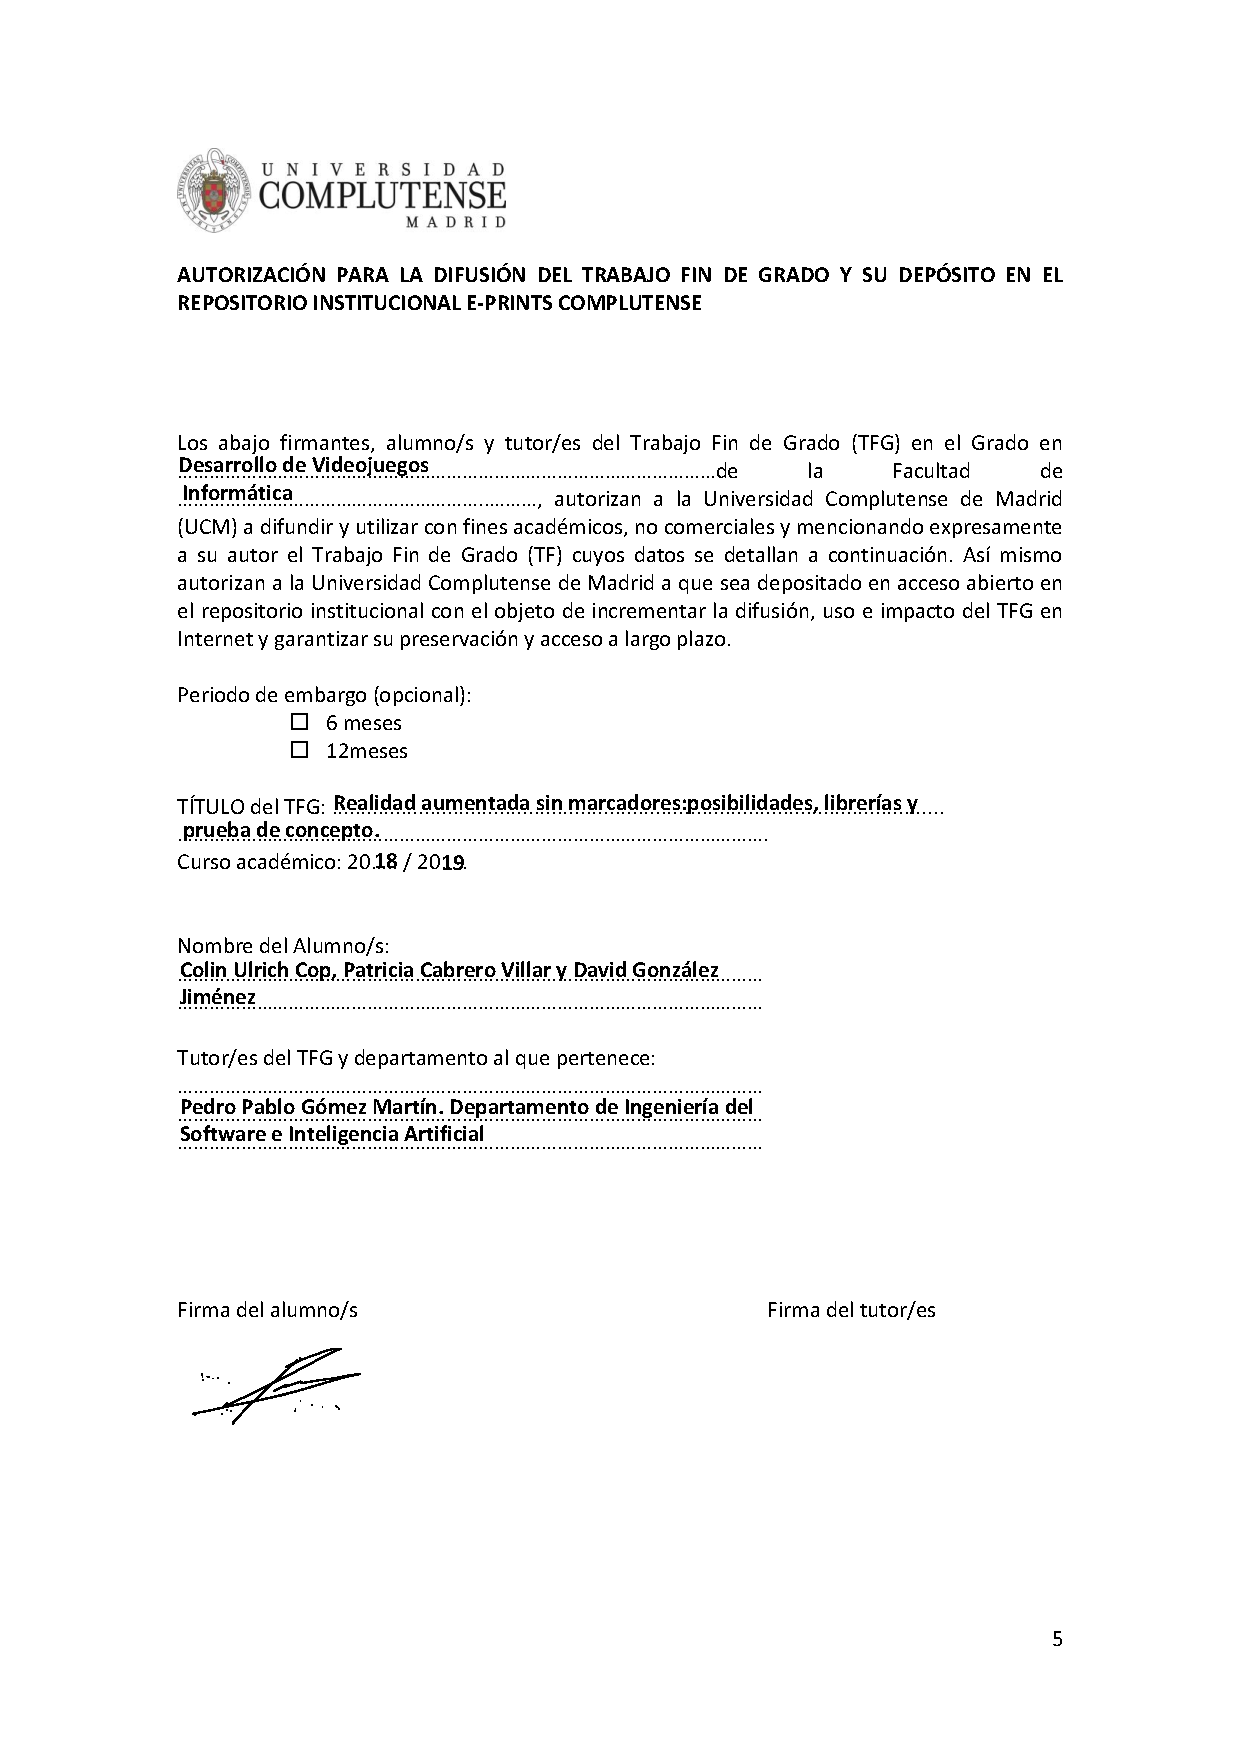
\includepdf[page=1]{Data/Autorizacion.pdf}
%\newpage
\chapter*{Agradecimientos}
\noindent

\indiceTFG
\newpage
\chapter*{Acrónimos}

\begin{itemize}
\item RA: Realidad aumentada
\item SDK: Software development kit (Kit de Desarrollo de software) 
\item SLAM: Simultaneous localization and mapping 
\item HMD: Head Mount Display 
\item API: Application Programming Interface 
\item IDE: Integrated Development Environment (Entorno de desarrollo integrado)
\end{itemize}

\noindent

%%%%%%%%%%%%%%%%%%%%%%%%%%%%%%%%%%%%%%%%%%%
%%%%%%%%%%%%%%%%%%%%%%%%%%%%%%%%%%%%%%%%%%% Parte 2
% - Resumenes
\newpage
\chapter*{Resumen}
\addcontentsline{toc}{chapter}{Resumen}
La realidad aumentada (RA) se ha convertido en la última década en una tecnología accesible a millones de usuarios a través de sus dispositivos móviles. Basada inicialmente en el uso de marcadores, hoy en día existen algoritmos que permiten su uso sin marcadores que, pese al éxito de juegos como Pokemon Go, no han terminado de despegar de manera general.\\

Este trabajo de fin de grado plantea un análisis de las posibilidades de la realidad aumentada sin marcadores. A lo largo del proyecto se exploran y estudian las librerías existentes, de cara a descubrir sus similitudes y diferencias realizando pequeñas pruebas de concepto. Con los resultados obtenidos de este estudio se han realizado tres aplicaciones que explotan las características de las librerías y las tecnologías estudiadas. La primera aplicación que se desarrolló ayuda al montaje de muebles en realidad aumentada. En esta aplicación se puso a prueba la librería ARCore y sus funcionalidades sin marcadores. En segundo lugar, se ha desarrollado un videojuego multijugador de cara a mostrar sus posibilidades en el campo haciendo uso de los puntos de ancla en la nube y la detección de planos. Por último, se ha creado una aplicación que permite disfrutar de la experiencia de una manera más natural usando las gafas de Aryzon\footnote{Gafas \textit{cardboard} que permiten tener una experiencia de realidad aumentada~\cite{Aryzon}.} interactuando con los objetos colocados en el plano escogido.\\
\\
\\

\section*{Palabras clave}
\addcontentsline{toc}{section}{Palabras clave}
Realidad aumentada, SLAM, ARCore, ARKit, RA sin marcadores, multijugador, seguimiento, detección de planos.

\noindent
\newpage
\chapter*{Abstract}
\addcontentsline{toc}{chapter}{Abstract}
In the last decade augmented reality has become an accessible technology to millions of users through their smartphones. Initially based on the use of markers, today there are algorithms capable of using it without markers, despite the success of games like Pokemon Go, this technology has not yet been consolidated.\\

This thesis presents an analysis of the possibilities of augmented reality, focused on markerless AR. Throughout the project, existing libraries are explored and studied, in order to discover their similarities and differences by developing small proofs of concept.\\ 

With the results obtained from this study, three applications will be developed. These applications will try to leverage all the potential of the libraries and the technologies studied. The first application helps the user in the furniture assembling process showing it step by step, using ARCore and its markerless functionalities.In order to show the augmented reality possibilities in videogames, a multiplayer videogame is developed using cloud anchors and plane detection.
Finally, the last application allows us to interact with the environment in a more natural way using Aryzon\footnote{Cardboard glasses that allow us to have an augmented reality experience.\cite{Aryzon}} glasses interacting with the objects placed in the chosen plane.
\\
\\
\\

\section*{Keywords}
\addcontentsline{toc}{section}{Keywords}
Augmented reality, SLAM, ARCore, ARKit, markerless AR, multiplayer, tracking, plane detection
\noindent
\noindent


% - Capítulos
\parindent=0em
\chapter{Introducción}
\pagenumbering{arabic}
\noindent
\section{Motivación}
En los últimos años la realidad aumentada se ha convertido en una tecnología madura y presente en la mayoría de los usuarios. Apoyada por el auge de dispositivos móviles inteligentes y la mejora de los componentes de estos la realidad aumentada es adoptada cada vez más por un mayor público. Se trata de un tema de actualidad recurrente y de referencia en múltiples productos de innovación.\\
Se estima que el tamaño del mercado de la RA crecerá de 3.5 mil millones en el 2017 a más de 198 mil millones de dólares en el 2025. En los años próximos se espera que revolucione mercados como son el arte, la educación, la publicidad, procesos de fabricación y montaje, turismo y especialmente el mundo de los videojuegos entre otros. Debido a este gran crecimiento del sector es un excelente tema para tratar de cara a conocer las limitaciones y puntos a destacar de cada una de las tecnologías existentes en la actualidad. 
\section{Objetivos}
El objetivo principal del desarrollo de este proyecto será conocer las posibilidades y limitaciones de las librerías de realidad aumentada sin marcadores existentes en la actualidad. En base a este objetivo se fijaron los siguientes objetivos específicos:
\begin{enumerate}
\item Investigación de las principales librerías de realidad aumentada sin marcadores.
\item Implementación de pruebas de concepto de cada una de ellas para analizar los pros y contras.
\item Análisis de los resultados obtenidos de las pruebas de concepto.
\item Planteamiento e implementación de diferentes aplicaciones de realidad aumentada sin marcadores en función de los resultados obtenidos en el análisis.
\item Desarrollar una aplicación/concepto de realidad aumentada en multijugador con los cloud anchors.
\end{enumerate}

\section{Metodología}
Para llevar a cabo estos objetivos se investigará a través de fuentes en internet, artículos científicos, estudios previos y libros, todos ellos reflejados en la bibliografía y webgrafía. Estos recursos serán la base de la fundamentación del proyecto y por ello se abrirán dos vías de investigación principales: se analizará por una parte acerca de las diferentes librerías de desarrollo en realidad aumentada y por otra las diferentes aplicaciones en el mercado de esta tecnología.\\

La revisión bibliográfica que se llevará a cabo vendrá definida por las dos áreas del conocimiento que se deben investigar de cara a desarrollar el objetivo principal planteado. En el campo del conocimiento técnico de la realidad aumentada se investigará a través de bibliografía recomendada por profesores de la Facultad de Informática de la Complutense. Los libros más significativos por tratar serán “\textit{Handbook of Augmented Reality}” de Borko Furht, “\textit{Augmented reality games I, Understanding the Pokémon GO phenomenon}” de Vladimir Geroimenko y “\textit{Augmented reality games II, The gamification of education, medicine and art}” de Vladimir Geroimenko.\\

Debido al continuo cambio que experimentan las tecnologías de realidad aumentada gran parte de la investigación se verá supeditada a artículos científicos, así como a la documentación de las distintas librerías que lideran el mercado.\\

Una vez completada la investigación teórica se testearán diferentes aplicaciones ya existentes con el objetivo de encontrar sus fortalezas y debilidades. A través de estas conclusiones se podrá llevar a cabo una prueba de concepto más solida y veraz evitando cometer errores anteriormente observados.\\
Se buscará conocer las características específicas de las librerías escogidas delimitando los pros y contras de cada una de ellas. Para identificarlas se realizará un test definido y cerrado, poniendo a prueba las diferentes librerías en el mismo dispositivo de cara a establecer una comparativa entre todas. Estas aplicaciones test se desarrollarán cuando sea posible en el entorno Unity.\\
Por último, se desarrollarán tres aplicaciones de mayor nivel de complejidad que nos permitan explotar las virtudes de tres librerías diferentes de cara a mostrar y fijar las conclusiones extraídas del anterior estudio.\\

A continuación, se detallan las tecnologías que se utilizarán a lo largo del desarrollo del proyecto.\\

Para la creación de las aplicaciones, se utilizará como entorno de desarrollo principalmente \textbf{Unity 2019.3}, uno de los motores de videojuegos punteros y referentes en la industria. Gracias a su versatilidad e interfaz intuitiva nos permitirá iterar rápidamente a lo largo de los test y pruebas de concepto. Este motor es uno de los escogidos por la facultad para estudiar a lo largo del grado de desarrollo de videojuegos con lo que nos resultará más cómodo y familiar, favoreciendo de nuevo la agilidad en el desarrollo.\\

Como IDE \footnote{IDE: Integrated Development Environment (Entorno de desarrollo integrado)}  se utilizará \textbf{Visual Studio 2019} acompañado por Visual Studio Tools para Unity una extensión gratuita de Visual Studio que lo convierte en una completa herramienta con la que desarrollar aplicaciones y juegos multiplataforma con Unity. Esta herramienta permite la integración de Visual Studio con el editor de Unity haciendo más eficaz el desarrollo.\\
El sistema de control de versiones escogido será \textbf{Github} ya que estamos habituados a la plataforma y nos permite integrarlo con herramientas como Visual Studio y Microsoft Teams.\\

La herramienta de seguimiento de tareas y comunicación entre el equipo escogida será \textbf{Microsoft Teams} dada su versatilidad y posibilidad de añadir herramientas.\\

Gracias a todas estas metodologías tanto prácticas, teóricas y técnicas y a las se lograrán cumplir los objetivos propuestos.\\

\section{Plan de trabajo}
La primera parte del trabajo consistirá en informarnos e investigar sobre las librerías de RA sin marcadores que lideran el mercado esta parte se realizará conjuntamente por los tres. Se estudiarán las diferentes tecnologías que componen la experiencia de la RA en los dispositivos móviles para entender cómo funciona a bajo nivel y estar actualizados con la demanda del mercado de cara a poder hacer una prueba de concepto verosímil con las aplicaciones de RA actuales. \\

En una segunda parte, después de identificar las librerías que existen en el mercado, se probarán (las que sean posibles) teniendo en cuenta los dispositivos y plataformas soportadas por cada una de ellas, a su vez se tendrá en cuenta la existencia de una licencia gratuita o de prueba. Se desarrollarán diversas aplicaciones de carácter básico a modo de test, éstas nos permitirán poner a prueba cada una de las principales librerías de realidad aumentada sin marcadores, comprobando su eficiencia. Los test serán ejecutados en las mismas condiciones lumínicas y con el mismo dispositivo de cara a obtener una mayor precisión en la comparación. En este caso nos dividiremos el desarrollo de los test de manera equitativa.\\

Una vez que se hayan encontrado las librerías que mejor se ajusten a nuestras necesidades, se desarrollarán las pruebas de conceptos las siguientes pruebas de concepto:
\begin{itemize}
\item Montar muebles de Ikea: se mostrará el proceso de montaje de un mueble en realidad aumentada. Ayudando al usuario a montar cada una de las piezas del proceso.
\item Juego multijugador usando \textit{cloud anchors}: se desarrollará un juego en el que poder poner a prueba las tecnologías de realidad aumentada sin marcadores combinada con puntos de localización en la nube permitiendo crear un juego multijugador.
\item Visualizador de modelos 3D con las gafas Aryzon: se hará uso de unas gafas de realidad aumentada tipo \textit{cardboard} en las que podremos ver superpuesto un modelo 3D, se podrá interactuar con el modelo 3D a través del mando de Xbox permitiendo rotarlo, escalarlo y moverlo.
\end{itemize}























\parindent=0em
\setcounter{chapter}{0}
\chapter{Introduction}
\noindent
\section{Motivation}
Over the last few years, the augmented reality has become a mature technology and it is accesible to a large amount of users. Supported by the rise of smartphones and the improvement of their components, augmented reality is increasingly being adopted by a larger audience. That is why this is an important and recurring topic in innovation products.

The augmented reality market is expected to grow from 3.5 million in 2017 to more than 198 million dollars by 2025~\cite{Statista}. In the next few years it is expected to transform several markets like art, education, advertising, manufacturing processes, tourism and specially videogames among others. It is an outstanding topic due to the growth of this sector and that is why we decided to study the limitations and capabilities of the currently available technologies.


\section{Objectives}
The main goal of the thesis will be determining and studying the capabilities and limitations of the currently available markerless augmented reality libraries. In order to accomplish this, we established the following objectives:

\begin{enumerate}[label={\arabic*.}]
\item Research and study of cutting-edge markerless augmented reality libraries.
\item Deployment of simple applications with each library in order to find its pros and cons.
\item Analysis of the results achieved by the previous applications.
\item Approach and implementation of different markerless augmented reality proof of concept based on the previously achieved results.
\item Development of a multiplayer augmented reality application.
\end{enumerate}


\newpage
\section{Work methodology}
To carry out these goals, we will investigate through internet sources, scientific articles, previous studies and books; all of them are reflected in the bibliography and webgraphy. These resources will be the basis of the project's foundation and that is why two main research channels will be opened: on one hand we will research and analyze the different augmented reality development libraries and on the other the different applications in the market for this technology.\\


The bibliographical review that will be carried out will be defined by two areas of knowledge that must be investigated in order to develop the main objective. In order to acquire technical knowledge of augmented reality, we will investigate through bibliography recommended by professors of the Complutense IT faculty. The most relevant books will be Borko Furht's “Handbook of Augmented Reality”, Vladimir Geroimenko‘s “Augmented reality games I, Understanding the Pokémon GO phenomenon” and “Augmented reality games II, The gamification of education, medicine and art”.\\

Due to the continuous change experienced by augmented reality technologies, the research will be strongly bounded to scientific articles, as well as to the documentation of the different libraries that lead the market.\\

Once the bibliographical research is completed, different existing applications will be tested in order to find their strengths and weaknesses. Thanks to these conclusions we will carry out a more solid and truthful proof of concept, avoiding previously observed mistakes.\\

We will seek to know the specific characteristics of the chosen libraries delimiting the pros and cons of each of them. To identify them, we will perform several defined and closed tests, testing the different libraries in the same device in order to establish a comparison between them. These test applications will be developed whenever possible in the Unity environment.\\

Finally, three applications of greater complexity will be developed that will allow us to exploit the virtues of different libraries in order to show and establish the previous study conclusions.\\

Unity \textbf{2019.2} and \textbf{2018.3} will be used as our development environment, as it is one of the leading videogame engines and it is a reference in the industry. Thanks to its versatility and intuitive interface it will allow us to iterate quickly throughout the tests and proofs of concept. We will be more comfortable with this engine as it is the one chosen by the faculty to study throughout the degree of videogame development, facilitating again the agility in development.\\

\textbf{Visual Studio 2019} will be used as our IDE, accompanied by Visual Studio Tools for Unity, a free Visual Studio extension that makes it a complete tool with which to develop applications and multiplatform games with Unity. This tool allows the Visual Studio integration with Unity editor allowing us to develop more efficiently.\\

\textbf{Github} will be the system control version chosen, we are used to the platform and it allows us to integrate it with tools such as Visual Studio and Microsoft Teams.\\

The task tracking and communication tool between the team will be \textbf{Microsoft Teams} given its versatility and the possibility of adding tools.



\section{Work plan}
First of all we will work on researching and analysing cutting-edge markerless AR libraries. This part will be carried out jointly by the three of us. We will study the different technologies that make up the experience of AR on smartphones to understand how it works at a low level and thus be able to figure out the market demand in order to make a credible proof of concept with current RA applications.\vspace{\baselineskip}

Secondly, after identifying the libraries that exist in the market, those will be tested (those that are possible) considering the devices and platforms supported by each of them, also keeping in mind the licenses offered in each of them.

We will develop test applications with each library, these will allow us to evaluate each of the markerless augmented reality libraries, checking their efficiency. The tests will be executed in the same light conditions and with the same device in order to obtain a greater precision in the comparison. In this case we will divide the test development in an equitable manner.\vspace{\baselineskip}

Once the libraries that best fit our needs have been found, the following proofs of concept will be developed:
\begin{itemize}
\item \textbf{Assemble Ikea furniture}: the process of assembling a piece of furniture in augmented reality will be displayed. Helping the user in the assembling process.
\item \textbf{Multiplayer game}: we will develop a game in which we will combine markerless technology with cloud anchors (section~\ref{cloudAnchorsSection}) allowing us to create an online multiplayer game.
\item \textbf{3D models visualizer with Aryzon glasses} (section \ref{AryzonSection}): we will use cardboard augmented reality glasses in which we can see a 3D model overlapped with the real world, in the application the user will interact with the 3D model through the Xbox controller allowing to rotate, scale and move it.
\end{itemize}

























\chapter{Antecedentes y estado del arte}
\section{Definición}
Se llama realidad aumentada al conjunto de tecnologías que permite a un usuario ver contenido virtual superpuesto al mundo real mediante un dispositivo tecnológico. Las tecnologías de realidad virtual se diferencian en que sumerge al usuario dentro de un entorno completamente sintético, sin tener consciencia del mundo real que lo rodea. La Realidad Aumentada no sustituye la realidad, sino que la complementa y puede mejorar la experiencia en ciertos ámbitos.

\section{Historia}
\begin{wrapfigure}{r}{0.5\textwidth}
    \centering
    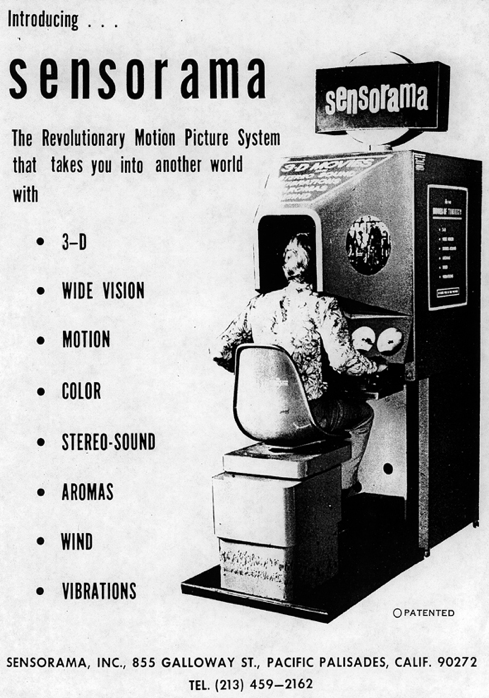
\includegraphics{Images/Sensorama.png}
    \caption{Cartel publicitario de la máquina Sensorama}
    \label{fig:Sensorama}
\end{wrapfigure}

En la década de 1950, surgió por primera vez el término realidad aumentada cuando Morton Heilig, un cinematógrafo, pensó en un prototipo de un cine que estimulara todos los sentidos del ser humano de manera efectiva. Años más tarde, concretamente en el 1962, Heilig construyó dicho prototipo, llamado Sensorama, se trataba de un cine inmersivo y novedoso que incluía funcionalidades como 3D, visión angular (actualmente conocido como IMAX), vídeo en color, sonido en estéreo, además de estimular otros sentidos con aromas, viento, y vibraciones como podemos observar en la figura \ref{fig:Sensorama}.\\
\\
\\

\begin{wrapfigure}{r}{0.5\textwidth}
    \centering
    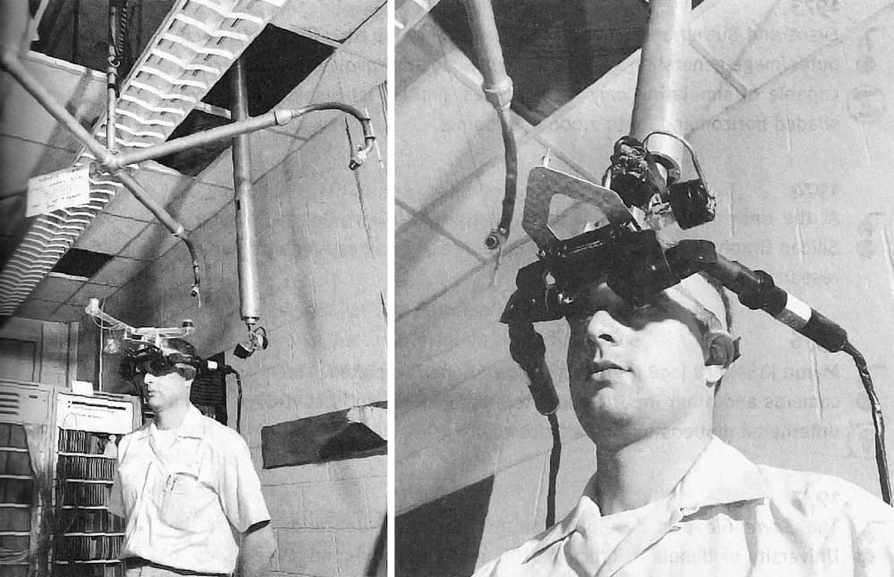
\includegraphics[width=0.48\textwidth]{Images/HumanMountDisplay.png}
    \caption{Ivan Sutherland “Espada de Damocles” 1968.}
    \label{fig:EspadaDamocles}
\end{wrapfigure}

En el 1968, Ivan Sutherland, inventó el HMD (\textit{Human Mounted Display}), siendo así, el primer sistema que permitía ver las aristas de sencillos objetos 3D (\textit{Wireframe}) en tiempo real. Empleaba dos sistemas de \textit{tracking} para calcular el registro de la cámara; uno mecánico y otro basado en ultrasonidos.\\
\\
\\
\\
\\


Sin embargo, no fue hasta 1992 cuando se acuñó el término de Realidad Aumentada por Tom Caudell y David Mizell, dos ingenieros de Boeing que proponían el uso de esta novedosa tecnología para mejorar la eficiencia y experiencia de las tareas realizadas por operarios humanos asociadas a la fabricación de aviones.
La aparición del primer videojuego en realidad aumentada ocurrió en el año 2000. Bruce Thomas demostró en el ISWC (The International Symposium on Wearable Computers) su videojuego ARQuacke. El sistema empleaba una brújula digital, un receptor de GPS y métodos de visión basados en marcas \cite{ARToolkit}. Los jugadores tenían que llevar una especie de ordenador portátil a la espalda, un casco de visión estereoscópica y un mando de dos botones.\cite{ARQuake}

\begin{figure}[ht]
    \centering
    \begin{minipage}{0.32\textwidth}
        \centering
        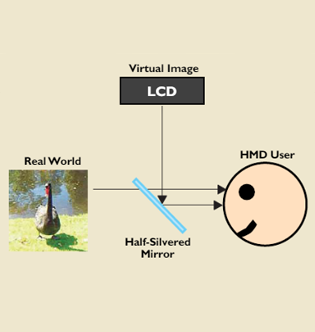
\includegraphics[width=\linewidth]{Images/ARQuake_HIW.png}
        \caption{Funcionamiento del Head Mounted Display}
    \label{fig:HIWARQuake}
    \end{minipage}\hfill
    \begin{minipage}{0.32\textwidth}
        \centering
        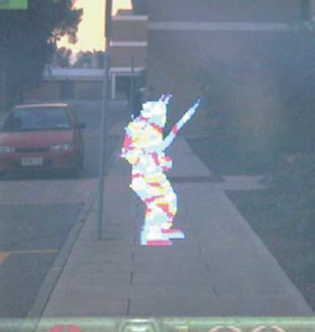
\includegraphics[width=\linewidth]{Images/ARQuake_Example.png}
    \caption{Ejemplo de ARQuake}
    \label{fig:Ex_ARQuake}
    \end{minipage}
        \begin{minipage}{0.32\textwidth}
        \centering
        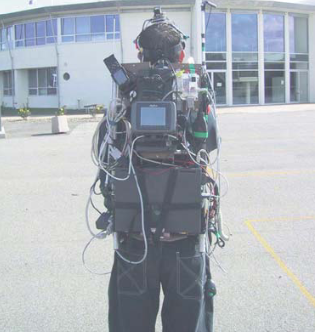
\includegraphics[width=\linewidth]{Images/ARQuake_Dispositivo.png}
    \caption{Dispositivo utilizado para ARQuake}
    \label{fig:Dispositivo_ARQuake}
    \end{minipage}
\end{figure}

\subsection{Immersive computing}
En 2007, en el ISMAR(Simposio internacional de realidad aumentada y mixta), Klein y Murray presentan el algoritmo PTAM (Parallel Tracking and Modeling) una variante al SLAM, que separa la localización y el mapeado en hilos diferentes. El SLAM es un algoritmo que sirve para que localizar la posición dentro de un entorno y modelarlo, más tarde lo explicaremos mas a fondo. Separar estos dos procesos en hilos diferentes permitía conseguir unos resultados en tiempo real muy sólidos.\\

\begin{wrapfigure}{r}{0.5\textwidth}
    \centering
    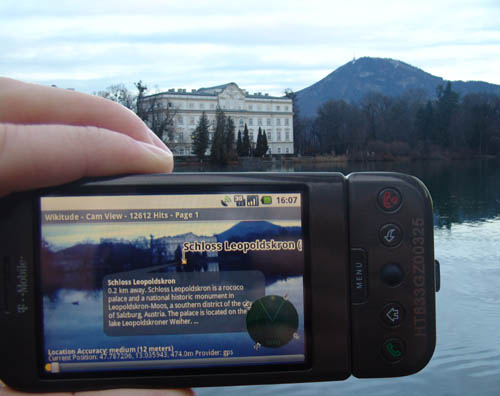
\includegraphics[width=0.48\textwidth]{Images/Wikitude_Example.jpeg}
    \caption{Wikitude App 2008}
    \label{fig:wikitude2008}
\end{wrapfigure}
En 2008 se creó Wikitude, una aplicación que utilizaba el GPS para mostrarte información de la Wikipedia según el lugar en el que estuvieras, pudiendo aprender datos sobre monumentos, esculturas o construcciones que te fueras encontrando.\\
\\
\\
\\
\\
\\
\\
\\
\\

Un año más tarde, en 2009, desarrolló el videojuego ARhrrrr del género shooter, el primer videojuego en realidad aumentada para smartphone con contenido 3D de alta calidad. Se generaba un mapa 3D sobre un marcador, y el objetivo era rescatar a los humanos de la ciudad y matar a los zombies. 

En el mismo año, el estudio español Novorama crea el videojuego de PSP (Portable PlayStation) Invizimals, un éxito mundial, vendiendo más de 8 millones de copias en todo el mundo en el primer trimestre de 2010. Este juego usaba la cámara addicional que se conectaba a la PSP, y con marcadores se registraba la posición del micro.

\subsection{Project Tango}
En 2014, Project Tango nació como uno de los primeros desarrollos de realidad aumentada pensado para ser distribuido mundialmente en los smartphones. En 2015, Tango pasa a formar parte de Google. El objetivo era crear un dispositivo portátil que permitiese mapear espacios 3D. Esta tecnología solo se desarrolló para el dispositivo Phab2 Pro de Lenovo, el cual incluía un mayor número de cámaras, concretamente 3.
Las tres funcionalidades principales para el desarrollo de esta tecnología han sido:
\begin{itemize}
\item Seguimiento del movimiento: Se trata del uso de las características visuales del entorno combinadas con los datos proporcionados por los sensores de movimiento incorporados en el teléfono, el acelerómetro y por el giroscopio, teniendo como objetivo realizar un seguimiento de los movimientos hechos del dispositivo. 
\item Reconocimiento del ambiente: Tango almacena la información del entorno que le rodea, buscando los puntos característicos en cada fotograma que recibe de las cámaras (más adelante explicaremos con más detalle cómo funciona el reconocimiento del ambiente).
\item Percepción de profundidad: Gracias a las cámaras especiales que incorpora el dispositivo, Tango puede calcular tamaños y distancias en el entorno que se encuentra. 
\end{itemize}
Después de 3 años, en 2017, Google decide cerrar el desarrollo de Tango y se centra en su tecnología actual, ARCore, que es el competidor directo de ARKit, la librería de Apple.

\section{Aspectos técnicos}
\subsection{Descripción}
La realidad aumentada es una tecnología que permite entremezclar el mundo virtual con el mundo, añadiendo la información virtual a la información física ya existente en tiempo real, permitiendo al usuario comprender mejor el entorno que le rodea. Hace unos pocos años, con la aparición de los dispositivos móviles más potentes y las librerías gratuitas de realidad aumentada, el desarrollo de esta tecnología se ha vuelto muy accesible para cualquier desarrollador. Esto implica en el número de ideas y aplicaciones que se generan cada día, que va aumentando drásticamente con el paso de los años.\\
En la actualidad existen tres tipos de realidad aumentada:
\begin{itemize}
\item Realidad Aumentada con marcadores (2D y 3D): Los marcadores pueden ser imágenes impresas o dibujos en los que la aplicación reconoce el marcador y activa la experiencia sobre dicho marcador.
\item Realidad Aumentada sin marcadores: Esta es la tecnología más novedosa, ya que combina diferentes tecnologías como (SLAM, seguimiento del movimiento, reconocimiento del ambiente, detección de planos ...) para proyectar el objeto y mantenerlo en el mismo punto de anclaje sin ayuda de ningún marcador.
\item Realidad Aumentada por Geolocalización: Este tipo de experiencias vinculan a la RA con una ubicación geolocalizada específica. Normalmente se utilizan en exteriores y proporcionan información contextual sobre el ambiente que nos rodea.
\end{itemize}
Las posibilidades de la realidad aumentada sin marcadores están en pleno auge y cada vez aparecen más aplicaciones que mejoran la experiencia de usuario y facilitan el trabajo en algunos sectores como puede ser la fábrica, la arquitectura, la medicina, la educación y muchos más.

\subsection{Métodos de tracking}
El Tracking es como conocemos al proceso de localización espacial del usuario en un entorno. Es uno de los aspectos clave en el desarrollo de aplicaciones de realidad aumentada ya que cuanto mejor sea la estimación de la posición y orientación del dispositivo sensor, mejores y más acertados serán los resultados y la inmersión por parte del usuario.\cite{BostanciTrackingMethods}\\
El cálculo del \textit{tracking} se encarga de posicionar la cámara relativamente a los objetos de la escena. Existen multitud de tecnologías y métodos para llevarlos a cabo, siendo los más comunes sensores mecánicos, magnéticos, sónicos, dinámicos y basados en visión. Éstos últimos son los más extendidos, ya que la mayoría de los dispositivos desde los que se despliegan las aplicaciones de realidad aumentada, como móviles o tablets, disponen de una o varias cámaras. \cite{ARToolkit}\\
El \textit{tracking} basado en cámaras de visión es un subcampo del \textit{tracking} 3D, en el que se utilizan algoritmos de visión por ordenador para obtener de la manera más precisa posible el posicionamiento de seis grados de libertad del dispositivo (tres grados de posición y otros tres de orientación.\\
En este tipo de posicionamiento es necesario disponer de un conjunto de marcadores o referencias tridimensionales para situar la cámara con respecto a ellas. Aunque recientemente se ha tendido a utilizar en menor medida los marcadores físicos para dar una experiencia más rápida y cómoda al usuario, han sido una herramienta imprescindible en los primeros pasos de la realidad aumentada para la obtención de la localización relativa de la cámara.
Según David Marimón\cite{TrackingThesis}, fundador y director general de Catchoom, se pueden distinguir dos aproximaciones distintas a la hora del tracking: los métodos Bottom-Up y los Top-Down. 

\subsubsection{Bottom-Up}
Las aproximaciones del tipo Bottom-Up pretenden obtener la posición del dispositivo basándose en la información que recibe a través de la cámara.
Para este método de tracking la posición y orientación se calculan en base a la obtención de características geométricas de objetos y sus relaciones. Dependiendo de los datos procesados, el seguimiento puede ser con marcas o sin ellas.\\
El tracking basado en marcas era el método más extendido en los inicios de la realidad aumentada. Hace sus cálculos con la ayuda de marcadores físicos que en su mayoría presentan un gran contraste entre blanco y negro para que los sensores puedan percibirlos con mayor facilidad. Existen también marcadores que usan códigos de colores y diferentes formas geométricas, aunque después de ser sometidos a prueba se comprobó que los más sólidos eran los marcadores cuadrados. Por otra parte, este método es especialmente sensible a la oclusión, ya que cuando se pierde el marcador, es imposible calcular la posición del dispositivo. Por este motivo, se han diseñado marcadores que puedan hacer frente a este problema con imágenes en escala de grises que completan marcas que no son visibles.\\
Paralelamente, el tracking sin marcas se basa únicamente en las características intrínsecas de la escena, estructuras físicas de fácil percepción como las esquinas de una mesa.\\
Existen técnicas en este campo que utilizan información sobre superficies planas detectadas en el campo de visión, siendo su principal inconveniente su alto coste computacional (actualmente este tipo de localización no lo pueden llevar a cabo todos los dispositivos del mercado).\\
Por otra parte, hay técnicas basadas en modelos. No están considerados marcadores porque son parte del medio natural, pero al igual que con éstos los cálculos se basan en el reconocimiento de los objetos que existen y que el programa está preparado para procesar.\\
Finalmente, existen métodos que actúan en escenarios donde no se es capaz de obtener planos o modelos. Se suelen emplear restricciones epipolares de las cámaras en movimiento. Sin embargo, esta técnica no es utilizada habitualmente por sus altos requisitos de cómputo.\\
\subsubsection{Top-Down}
Las aproximaciones del tipo Top-Down intentan estimar desde la posición actual del dispositivo si se está percibiendo lo que se esperaba. Es decir, primero se estima la posición y después se confirma esa estimación con los datos del medio.
En este caso, se emplean modelos del movimiento basados en filtros bayesianos para hacer una predicción de la localización del dispositivo. Partiendo de esta estimación, se busca mediante la cámara una serie de referencias parciales que corrijan la predicción y mejoren el posicionamiento del observador. Por ello, todos los modelos Top-Down se ven obligados a trabajar con filtros y modelos de asociación de datos.
El uso de estos filtros permite combinar varios métodos de tracking y mantener un registro constante de los objetos y la cámara, aunque los marcadores, modelos o planos sean parcialmente visibles por oclusión o se hayan escapado del campo de visión.
Además del seguimiento óptico, se han desarrollado numerosas alternativas con las que proporcionar otros métodos de localización (como los beacons o la ubicación del GPS) y así complementar y facilitar una localización más precisa y correcta. A las aproximaciones que se valen de varias de estas técnicas se las denomina métodos de fusión.

\subsection{Tecnologías implicadas en la RA sin marcadores}
El objetivo de la realidad aumentada es integrar contenido virtual en el mundo real. Idealmente, dicho contenido se tendría que comportar exactamente como uno real, esto requiere una información muy precisa sobre la posición del dispositivo que usa el usuario con respecto al objeto virtual. Para ello, se han desarrollado diferentes tecnologías que junto a los sensores de los teléfonos actuales (giroscopio, acelerómetro, sensor de luz) y a la cámara, permiten disfrutar de una experiencia casi ideal. \cite{ARCarmigniani} 

\subsubsection{SLAM(Simultaneuos localization and mapping)}
Mapeo y localización simultáneos se le llama a la tecnología que se basa en una serie de algoritmos complejos que utiliza los datos de los sensores para construir un mapa de un entorno desconocido y a su vez para saber dónde está localizado el dispositivo. Esta técnica es usada por robots y por vehículos autónomos. 
¿Cuál es el objetivo? Descubrir donde estoy. La tecnología SLAM, en el momento que empieza el algoritmo, no tiene ningún tipo de información del entorno. Normalmente, sólo tarda unos pocos segundos en crear un mapa aproximado del entorno con lo que calcula una posición inicial. Más adelante, el mapa creado va creciendo y mejorando en base a la información que obtiene desde el fotograma de la cámara.
Aunque este término empezó a aparecer en la década de los 90, las primeras implementaciones carecían de cámaras o sensores que proporcionaban información visual. En 2005 comenzó a abaratarse el coste de los ordenadores y de las cámaras, y los investigadores empezaron a combinar el SLAM con sensores visuales. Hasta este punto, esta tecnología estaba pensada para la navegación con robots en entornos desconocidos, hasta que en 2007 Georg Klein y David Murray vieron el potencial de usar esta tecnología en la realidad aumentada. \cite{MaxstMedium}

\subsubsection{Reconocimiento del ambiente}
Cuanto mejor entienda la aplicación como es el entorno que le rodea, mejor será la experiencia de usuario. En este apartado, también entra el reconocimiento de superficies, tanto horizontales como verticales. El funcionamiento de esta tecnología consiste en procesar cada fotograma obtenido por la cámara y encontrar puntos característicos, estos puntos pueden ser cualquier cosa que ayuden a identificar objetos (esquinas, líneas, bordes de objetos, colores, gradientes, etc…), por lo que si se intenta detectar un plano en una superficie donde el color sea uniforme, y carezca de textura o patrones, como puede ser una pared totalmente blanca, seguramente no funcione con normalidad \cite{ARCoreConcepts}. Con estos puntos, luego se construye una maya que va a servir como superficie en la escena de nuestra aplicación y con la cual podremos interactuar activándole las físicas y colisión.
\subsubsection{Estimación de la luz}
Esta tecnología es muy importante ya que aporta un nivel de detalle excelente, los modelos 3D virtuales se comportan como si fueran reales, se iluminan con la iluminación del mundo físico y emiten sombras. La estimación de la luz es posible gracias a la combinación de la información del seguimiento del movimiento y usando un algoritmo de análisis de imagen que determina la intensidad de la luz en la imagen del dispositivo. Cuanto más se mueva la cámara y más información recoja sobre el entorno, más precisos serán los datos de dónde viene la mayor fuente de luz, analizando el nivel de brillo de los píxeles de los fotogramas, por lo que se puede estimar la dirección en la que viene. A esta información se puede acceder desde Unity o el motor que se use, donde se le aplican los valores obtenidos a una la luz posicional.
\subsubsection{Oclusión}
El término oclusión se refiere a cuando un objeto nos impide ver otro objeto o imagen que hay detrás. Para disfrutar de una experiencia de realidad aumentada realista, esta tecnología es esencial, los objetos virtuales tienen que seguir esta regla, porque en el momento en el que cruza una persona delante del objeto, o cruzas la esquina, y sigues viendo el objeto virtual, se arruina la inmersión que podemos llegar a tener. Por lo que no sirve únicamente saber dónde está situado nuestro dispositivo con respecto al objeto, si no también hace falta saber si hay otro objeto o superficie en medio.\cite{articleOclusion}
\subsubsection{Detección de rostros}

Uno de los puntos más importantes de la realidad aumentada en la actualidad es la detección de caras y su reconocimiento.\\

Cada cara está compuesta por al menos 80 rasgos distinguibles, como la distancia que existe entre los extremos de la mandíbula, la profundidad de las cuencas oculares o la separación que hay entre los agujeros de la nariz. \cite{BBC_FacialRecognition}Los humanos somos especialmente buenos reconociendo estos rasgos porque tenemos una zona del cerebro dedicada específicamente a interiorizar patrones.
Basándonos en el funcionamiento del cerebro de una persona hemos desarrollado algoritmos que imitan estas asociaciones, dividiendo las caras en un conjunto de puntos de referencia a los que llamamos nodal points y buscando correspondencias con otras fotos tomadas anteriormente. El algoritmo que sigue un sistema para tratar de identificar si lo que está viendo es una cara pasa por comprobar si existe en la imagen un patrón similar al que formarían normalmente los rasgos más característicos de una cara, para después preguntarse de quién es esa cara. Sin embargo, no existen dos fotos de una misma persona que sean iguales, de manera que los algoritmos tienen que lidiar con 4 problemas fundamentales a la hora de reconocer la cara de una persona: el envejecimiento, la pose, la iluminación y las emociones.\\

En los últimos años se ha desarrollado un sistema de reconocimiento en 3D llamado Deepface, que es capaz de tomar una foto en 2D de un individuo y crear un modelo tridimensional. De esta forma, el sistema tendrá muestras de los rasgos faciales desde todos los ángulos disponibles, solucionando así el problema de la pose.\\

Por otra parte, el problema del envejecimiento también ha sido debidamente prevenido, ya que al crear la estructura 3D de la cara se tienen en cuenta los nodal points más importantes y que menos varían con el transcurso de los años, como son las curvas de los ojos, de la nariz o de la barbilla. Pero lo que realmente ha supuesto un avance en este campo es el Deep Learning, que es un sistema de algoritmos que guía al programa redirigiéndole si va por mal camino. Cada vez que asocia una cara correcta o incorrectamente, registra el proceso por el que ha pasado para realizar la comprobación y queda guardado en un mapa que va ampliándose sucesivamente con cada acierto o error del sistema. De esta manera, cuantas más conexiones se creen mayor será la fiabilidad a la hora de reconocer una cara.\\

Facebook por ejemplo se vale de este método para el reconocimiento facial y posee una red neuronal de más de 20 millones de nodos, con una fiabilidad del 97.35 \%(datos de 2015)\cite{Facebook_FacialRecognition} y que aun así es inferior a la capacidad de detección de una persona.\\\

Se espera que con la mejora de la tecnología el reconocimiento facial sea una forma de identificación tan válida como las huellas dactilares y que puedan identificarse las caras de las personas incluso en grabaciones de seguridad en calidad baja y sin color, así como un método de reconocer el género, edad y otras características del individuo para ofrecerle un servicio o producto más acorde con él en ámbitos como la publicidad.\\
\begin{figure}[H]
     \centering
     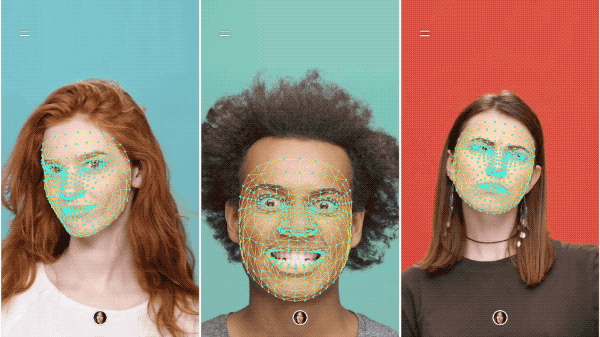
\includegraphics[width=0.7\textwidth]{Images/FaceRecognition.png}
     \caption{Detección de rostros}
     \label{fig:FaceRecognition}
 \end{figure}

\subsubsection{Puntos de ancla en la nube (Cloud Anchor)}
El Cloud Anchor es un mecanismo que permite a los usuarios de una aplicación de realidad aumentada añadir objetos virtuales a una escena. De esta manera múltiples usuarios pueden interactuar y ver los mismos objetos desde dispositivos distintos, pero compartiendo un mismo espacio físico. Su funcionamiento es muy similar al de los anchors comunes, que se utilizan para fijar un objeto en una posición, con la diferencia de que los Cloud Anchors se hospedan en los servidores de Google. De esta manera varios dispositivos pueden consultarlos para situar los objetos en la aplicación.\\

Para ser utilizados, la aplicación en cuestión tiene que tener conexión a internet.
Los Cloud Anchors son actualmente propios del SDK de ARCore, están soportados tanto en Android como en iOS (siempre que el dispositivo lo permita) y funcionan de la siguiente manera: ARCore tiene que generar primero un mapa de las proximidades del punto de ancla que será el centro de interés. Para ello, la cámara recopila información y características del entorno cercano desde diferentes ángulos y posiciones durante 10 segundos. Cuanto más precisa sea la información recopilada, mejor será la experiencia del usuario. Una vez transcurrido el tiempo, los parámetros del punto se hospedan en la nube y se establece el anchor, devolviendo el servidor un número de identificación único (el Cloud Anchor ID). Cuando otro usuario de la aplicación dirige su cámara hacia el mismo punto de interés, el Cloud Anchor procesa las características visuales del entorno físico desde el nuevo punto de vista. Estas características son comparadas con el mapa 3D que se ha generado anteriormente por el otro dispositivo y se establece la posición y orientación del nuevo usuario con respecto a ello para que pueda ver los objetos virtuales con la mayor precisión posible.\\

Para identificar un punto de ancla en la nube desde otro dispositivo se debe apuntar al lugar en que está situado sin importar la posición del dispositivo, siempre y cuando haya una línea recta entre ambos y no estén separados por una distancia superior a 10 metros.\\

En el caso de ARKit la tecnología para el usuario es igual, pero por dentro no funciona exactamente igual. ARKit no manda los datos a un servidor, si no que utiliza el framework MultipeerConnectivity de Apple para mandar la información del mapa (ARWorldMap) por una conexión cliente a cliente. \cite{Apple_CloudAnchor}\\

Cabe mencionar también que los Cloud Anchors tienen una serie de limitaciones en el almacenamiento y el acceso a los datos. Sólo pueden accederse hasta 24 horas después de haber sido colocados y 7 días después cualquier dato en la nube será borrado. El mapa hospedado en la nube no puede ser descargado por ningún usuario y no se puede determinar un lugar geográfico o reconstruir imágenes basándose en el mismo. Además, los datos que envía un dispositivo para que sean comparados con el mapa guardado no se almacenan nunca.\\

Para hacer un buen uso de ellos se debe evitar colocar puntos de anclado en superficies brillantes e intentar que la zona tenga una iluminación buena y consistente.

\section{Aplicaciones}
En este apartado se recogen las principales aplicaciones por sectores que existen de la realidad aumentada. Estas son la medicina, educación, arte, seguridad, publicidad, turismo, ecommerce y videojuegos.
\subsection{Medicina}
\cite{ARGames_Gamification}
\subsection{Educación}
\subsection{Arte}
\subsection{Fabricación}
\subsection{Publicidad}
\subsection{Turismo}
\subsection{Videojuegos}
\subsection{Comercios electrónicos(ecommerce)}
Los probadores virtuales están marcando tendencia en las nuevas generaciones de aplicaciones y estrategias de venta. Estas aplicaciones hacen uso de la realidad aumentada con tecnologías como el reconocimiento de rostros, reconocimiento de superficies, estimación de luces… Siendo punto de referencia en el mercado los siguientes ejemplos. 
\begin{enumerate}
\item \textbf{Ikea Place}\\
Esta aplicación permite al usuario ver el catálogo de Ikea y una vez seleccionado el elemento verlo en la habitación real con las dimensiones reales del objeto.
\begin{figure}[H]
     \centering
     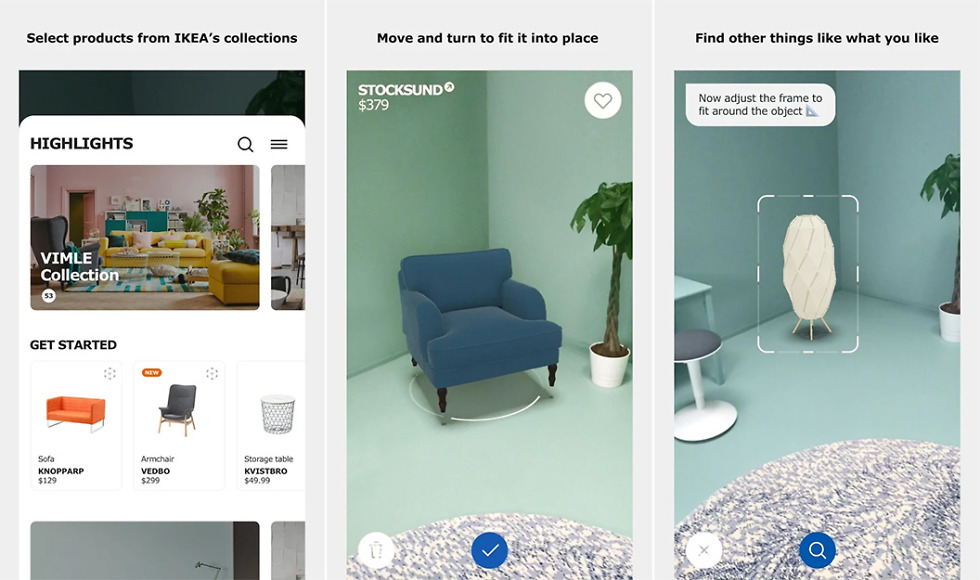
\includegraphics[width=0.6\textwidth]{Images/Ikea_App.jpeg}
     \caption{IKEA Place AR probador virtual}
     \label{fig:Ikea}
 \end{figure}
 \item
 \textbf{YouCam Makeup}\\
Esta aplicación es un excelente y conseguido ejemplo de ecommerce en el mundo de la belleza donde se aplica esta tecnología. La calidad del tracking del pelo es bastante razonable generando una experiencia agradable.
\begin{figure}[H]
    \centering
    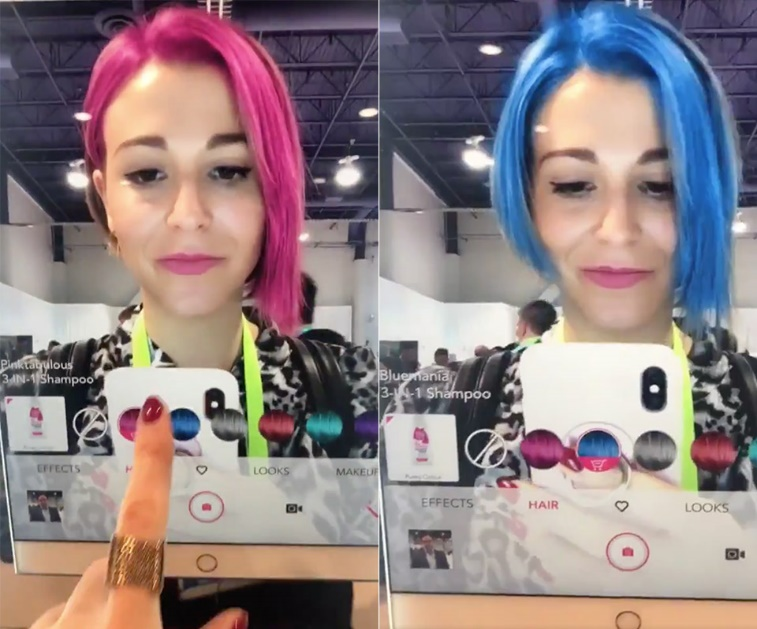
\includegraphics{Images/Loreal_App.jpeg}
    \caption{Imagen representativa de YouCam Makeup}
    \label{fig:YouCam}
\end{figure}
\item \textbf{L’Oreal (Modiface)}\\
Aplicación que permite al usuario maquillarse con los productos de L’Oreal en realidad aumentada, así como escoger el color que más pegue con sus prendas. Mostrando los productos relacionados a esa tonalidad y ofreciendo la posibilidad de comprarlos dentro de la aplicación.
\begin{figure}[H]
    \centering
    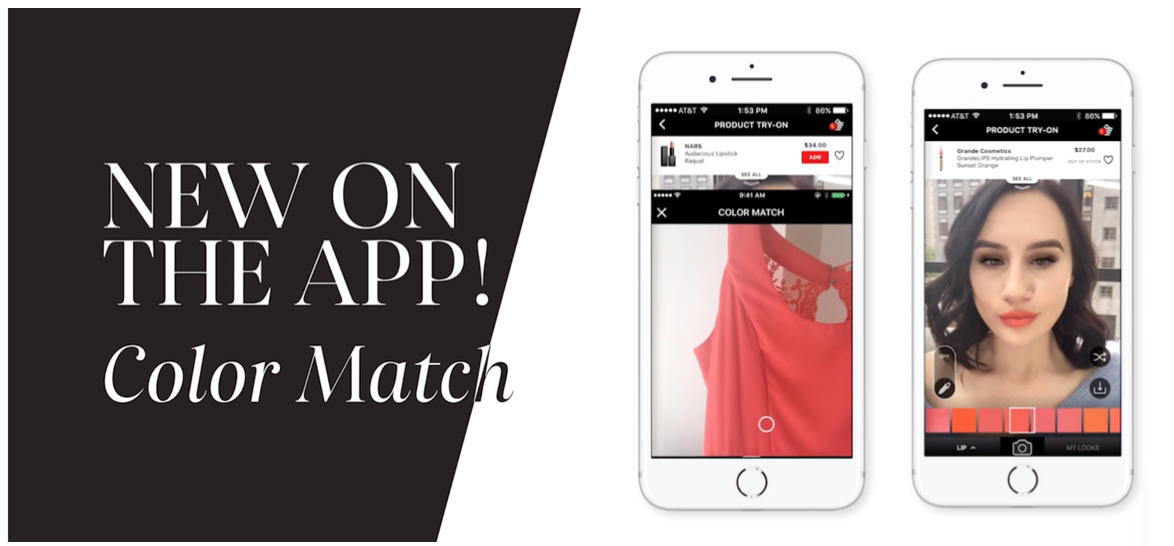
\includegraphics[width=0.7\textwidth]{Images/Loreal_App.png}
    \caption{Pantallas de ejemplo de la aplicación L'Oreal Modiface}
    \label{fig:Loreal}
\end{figure}
\end{enumerate}
\section{Experiencia de usuario en aplicaciones de RA sin marcadores}
\clearpage
\section{Librerías de realidad aumentada sin marcadores (SDK)}
En este apartado se describirán las principales tecnologías de realidad aumentada sin marcadores para más tarde estudiar las capacidades y posibilidades particulares de cada una de ellas en el apartado desarrollo.
Por cada librería se recogerán los siguientes datos:
\begin{itemize}
\item Breve descripción
\item Última versión
\item Funciones
\item Plataformas disponibles
\item Tipos de licencia
\end{itemize}
Luego se compararán todas juntas para ver las funcionalidades que tienen, las plataformas con las que son compatibles y los lenguajes que soportan.
\clearpage
\subsection{Wikitude}
\begin{figure}[H]
    \centering
    
\includegraphics[width=0.2\textwidth]{Images/Wikitude_Logo.png}
    \caption{Logo de Wikitude}
    \label{fig:Wikitude}
\end{figure}
Desarrollada por Wikitude GmbH, es una de las librerías pioneras en el mundo de la realidad aumentada. Lanzaron su primera aplicación en el 2008, desde entonces, son líderes del mercado. La versión que hemos usado ha sido Wikitude SDK 8.7.0 (2019-08-13).\cite{Wikitude}
Las principales funcionalidades son:
Geo AR (Puntos de anclaje vía GPS)
Reconocimiento de imágenes 2D (marcadores) 
Reconocimiento de objetos 3D
Las plataformas móviles soportadas son:
\begin{itemize}
\item Android
\item iOS
\item Windows
\item Unity
\item Cordova
\item Xamarin
\item Flutter
\item Titanium
\end{itemize}
Soporte para Smart Glasses:
\begin{itemize}
\item Epson Moverio
\item Hololens
\item Vuzix
\end{itemize}
Otras plataformas:
\begin{itemize}
\item React Native
\item Ionic
\item Adobe Air
\item Qt by Felgo
\item LBAR
\end{itemize}
Licencias:
\begin{itemize}
\item Wikitude Demo. Licencia de 30 días con marca de agua 499€
\item Wikitude SDK PRO (Sólo con marcadores y Geo AR). 1 año de licencia 1990€
\item Wikitude SDK PRO 3D (Paquete completo). 1 año de licencia 2490€
\end{itemize}


\subsection{ARKit}
\begin{figure}[H]
    \centering
    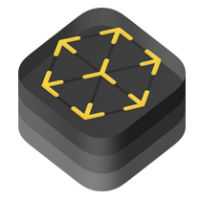
\includegraphics[width=0.2\textwidth]{Images/Arkit_Logo.jpeg}
    \caption{Logo de ARKit}
    \label{fig:ARKit}
\end{figure} 

Desarrollado por Apple, presentado en la Apple Worldwide Developers Conference de 2017.
La versión con la que trabajamos es la ARKit SDK 3.0.\cite{AppleDeve} A diferencia del resto, para usar esta librería en Unity, no hace falta descargar ningún plugin, viene incluido en el paquete de Unity ARFoundation 2.2.
Funcionalidades:
\begin{itemize}
\item Reconocimiento de imágenes 2D (marcadores)
\item Reconocimiento de objetos 3D
\item Reconocimiento de rostro (hasta 3 simultáneamente)
\item Oclusión
\item SLAM
\item Estimación de luces
\item Puntos de anclaje en la nube
\end{itemize}
Las plataformas soportadas son:
\begin{itemize}
\item iOS 
\item Unity (via ARFoundation)
\item Unreal Engine 4.\cite{Unreal}
\end{itemize}
La licencia es gratuita.

 
\subsection{ARCore}
 \begin{figure}[H]
    \centering
    
\includegraphics[width=0.2\textwidth]{Images/ARCore.jpeg}
    \caption{Logo de ARCore}
    \label{fig:ARCore}
\end{figure}

Desarrollado por Google, fue lanzado en febrero de 2018 como respuesta para competir contra ARKit de iOS. La versión con la que trabajamos es ARCore SDK for Unity v1.11.0 (2019-05-05).\cite{ARCore}
Funcionalidades:
\begin{itemize}
\item Reconocimiento de imágenes 2D (Marcadores)
\item Reconocimiento de objetos 3D
\item Reconocimiento de rostro.
\end{itemize}
\begin{itemize}
\item SLAM
\item Mapeado de áreas grandes
\item Estimación de luces
\item Puntos de anclaje en la nube
\end{itemize}
Las plataformas soportadas son:
\begin{itemize}
\item Android
\item Android NDK
\item Unity (Android, iOS)
\item Unreal Engine 4
\item iOS
\end{itemize}
La licencia para usar ARCore es completamente gratuita.

\subsection{Vuforia}
\begin{figure}[H]
    \centering
    
\includegraphics[width=0.2\textwidth]{Images/Vuforia.jpeg}
    \caption{Logo de Vuforia}
    \label{fig:Vuforia}
\end{figure}
Desarrollado por la empresa PTC, un proveedor tecnológico mundial de la plataforma líder de IoT (Internet of Things) y realidad aumentada. La versión que hemos utilizado ha sido Vuforia SDK Android 8.3.8 (2019-06-13).\cite{Vuforia}
Funcionalidades:
\begin{itemize}
\item Reconocimiento de imágenes 2D (Marcadores)
\item Reconocimiento de objetos 3D
\item Escáner de objetos 3D
\end{itemize}
Plataformas:
\begin{itemize}
\item Android
\item iOS
\item Windows
\item Smart Glasses
\end{itemize}
Licencias:
\begin{itemize}
\item Básica, 42\$ al mes.
\item Básica con base de datos en la nube para los marcadores 99\$ al mes.
\item Para la versión pro, la cual incluye todas las funcionalidades, hay que contactar y hacen presupuesto a medida para la empresa.
\end{itemize}

\subsection{Kudan}
 \begin{figure}[H]
    \centering
    
\includegraphics[width=0.2\textwidth]{Images/Kudan_Logo.png}
    \caption{Logo de Kudan}
    \label{fig:Kudan}
\end{figure}

Kudan es una empresa que se dedica al desarrollo de la realidad aumentada, virtual y mixta, además de la conducción autónoma, drones y robots. La versión que hemos utilizado ha sido la Kudan SDK Unity 1.6.0 (2019-07-16).\cite{Kudan}
Funcionalidades:
\begin{itemize}
\item Reconocimiento de imágenes 2D (Marcadores)
\item SLAM
\end{itemize}
Plataformas:
\begin{itemize}
\item Unity (Android, iOS)
\item iOS
\item Android
\end{itemize}
Licencias:
\begin{itemize}
\item AR Indie: Gratis. Pensado para la fase de desarrollo, protegido con marca de agua.
\item AR Business: 1500\$. Para las empresas con menos de un millón de dólares en ingresos.
\item AR Enterprise: Para las empresas con más de un millón de dólares en ingresos, hay que contactar con Kudan y proporcionan un presupuesto personalizado.
\end{itemize}


\subsection{MaxST}

 \begin{figure}[H]
    \centering
    
\includegraphics[width=0.2\textwidth]{Images/Maxst_Logo.jpeg}
    \caption{Logo de Maxst}
    \label{fig:Maxst}
\end{figure}

Maxst se fundó en 2010 y se dedica a la investigación y desarrollo de la tecnología de realidad aumentada, han lanzado Maxst AR SDK, el cual hemos probado en la versión MaxstARSDK\_Unity 4.1.3. \cite{Maxst}
Funcionalidades:
\begin{itemize}
\item Reconocimiento de imágenes 2D (Marcadores)
\item Reconocimiento de objetos 3D
\item Reconocimiento de códigos de barras y QR.
\end{itemize}
Plataformas:
\begin{itemize}
\item Unity (Android,iOS)
\item Android
\item iOS
\item Windows
\item macOS
\item Epson MOVERIO BT-300,350 y ODG R-7
\end{itemize}
Licencias:

\begin{itemize}
\item Free. Gratis, para uso no comercial, incluye marca de agua.
\item Pro-one. Para aplicaciones con menos de 100k descargas (no incluye actualizaciones). Pago único de 499\$ 
\item Pro-Subscription. Subscripción anual, incluye actualizaciones 599\$ por año
\item Enterprise. Para aplicaciones con más de 100k de descargas. Hay que contactar con Maxst para recibir un presupuesto.
\end{itemize}


\subsection{8th Wall}
\begin{figure}[H]
    \centering
    
\includegraphics[width=0.2\textwidth]{Images/8thWall_Logo.jpeg}
    \caption{Logo de 8th Wall}
    \label{fig:8th Wall}
\end{figure}

8th Wall desarrolla dos productos diferentes, 8th Wall Web y 8th Wall XR for Unity. El producto que vamos a analizar en este caso es el 8th Wall XR for Unity 11.2.6.519, para que la comparación entre las librerías sea mas precisa, ya que la potencia que tiene en navegador es menor a la que puede llegar a tener una aplicación de Unity. \cite{8thWall}
Funcionalidades:
\begin{itemize}
\item Reconocimiento de imágenes 2D (Marcadores)
\item 6 grados de libertad.
\item SLAM
\item Estimación de la luz
\end{itemize}

Plataformas:
\begin{itemize}
\item Unity (Android, iOS)
\item Web (A-Frame, BabylonJS, Sumerian, three.js)
\end{itemize}
El uso de 8th Wall XR de Unity es gratuito. En el caso de 8th Wall Web, la licencia se cobra según las visitas en la web. Aparte, se necesita una licencia de desarrollador que cuesta 250\$/mes.\\

\begin{center}
\begin{tabular}{| c| c |c| c |}
 Pago por visita (PPV)&	Paquete estándar&PPV de alto tráfico&Paquete alto tráfico \\
 \hline
  1000\$/mes	& 3000\$/mes	& 6000\$/mes &	6000\$/mes \\  
  \hline
 0 visitas incluidas &	500k visitas incluidas&	0 visitas incluidas	&5M visitas incluidas\\
 \hline
 0.01\$/visita&	0.01\$/visita extra&	0.0025\$/visita&	0.0025\$/visita extra\\
 \hline
\end{tabular}
\caption{Licencias 8th Wall}
\end{center}
\\

\subsection{Easy AR}
\begin{figure}[H]
    \centering
    
\includegraphics[width=0.2\textwidth]{Images/EasyAR.png}
    \caption{Logo EasyAR}
    \label{fig:my_label}
\end{figure}

EasyAR es una compañía china que lleva en el mercado desde 2016. Hemos probado la versión EasyARSense Unity SDK v3.0.1(2019-07-07)\cite{EasyAR}
Funcionalidades:
\begin{itemize}
\item Reconocimiento de imágenes 2D (Marcadores)
\item Reconocimiento de objetos 3D
\item SLAM
\item Grabación de pantalla
\end{itemize}
Plataformas soportadas:
\begin{itemize}
\item Unity (Android, iOS)
\item Android
\item iOS
\item Windows
\end{itemize}
Licencias:
\begin{itemize}
\item EasyAR SDK Basic. Gratis
\item EasyAR SDK Pro. Añade el reconocimiento de objetos 3D, la grabación de pantalla y reconocimiento de más de un marcador simultáneo
\item EasyAR SDK Pro trial. Lo mismo que el Pro, pero limitado a 100 usos por día.
\end{itemize}


\subsection{ARFoundation}
\begin{figure}[H]
    \centering
    
\includegraphics[width=0.2\textwidth]{Images/Unity_Logo.jpeg}
    \caption{Logo Unity}
    \label{fig:my_label}
\end{figure}

Este último no se trata exactamente de una librería, es un paquete de Unity (aún en fase experimental) que integra una API de alto nivel (wrapper) que permite tener el mismo código funcional para ARCore y ARKit, según si exportamos el proyecto en Android o en iOS. La versión más reciente es ARFoundation 2.2 (Unity 2019.1), la cual incluye ARKit 3.\cite{ARFoundation}\\
Soporta las mismas funcionalidades que ARCore y ARKit:
\begin{itemize}
\item Reconocimiento de imágenes 2D (marcadores)
\item Reconocimiento de objetos 3D.
\item Reconocimiento de rostro 
\item Oclusión (iOS con ARKit)
\item SLAM
\item Mapeado de áreas grandes (ARCore)
\item Estimación de luces
\item Puntos de anclaje en la nube
\end{itemize}

Plataformas soportadas:
\begin{itemize}
\item Unity (Android, iOS)
\end{itemize}

Su licencia, al igual que ARCore y ARKit, es gratuita.

\noindent

\chapter{ Realidad aumentada sin marcadores }\label{RASinMarcadores}

\section{Aspectos técnicos}
\subsection{Descripción}
La realidad aumentada es una tecnología que permite mezclar el mundo virtual con el mundo físico, añadiendo la información virtual a la información física ya existente en tiempo real, permitiendo al usuario comprender mejor el entorno que le rodea~\cite{ARCarmigniani}. En la última década, con la aparición de los dispositivos móviles más potentes y las librerías gratuitas de realidad aumentada, el desarrollo de aplicaciones de RA se ha vuelto muy accesible para cualquier desarrollador. Esto implica un aumento drástico en el número de ideas y aplicaciones que surgen día a día.\\

En la actualidad existen tres tipos de seguimiento en la realidad aumentada:
\begin{itemize}
\item \textbf{Realidad aumentada con marcadores (2D y 3D)}: Los marcadores son imágenes impresas, dibujos o objetos previamente escaneados en los que la aplicación reconoce el marcador y activa la experiencia sobre dicho marcador. 

\item \textbf{Realidad aumentada sin marcadores}: Esta es la tecnología más novedosa, ya que combina diferentes tecnologías como SLAM (detallado en el apartado~\ref{SLAMsection}), seguimiento del movimiento, reconocimiento del ambiente o detección de planos para proyectar el objeto y mantenerlo anclado en el mismo punto sin ayuda de ningún marcador.

\item \textbf{Realidad aumentada por geolocalización}: Este tipo de experiencias vinculan a la RA con una ubicación geolocalizada específica. Normalmente se utilizan en exteriores y proporcionan información contextual sobre el ambiente que nos rodea.
\end{itemize}
Las posibilidades de la realidad aumentada sin marcadores están en pleno auge y cada vez aparecen más aplicaciones que mejoran la experiencia de usuario y facilitan el trabajo en algunos sectores como puede ser la industria, la arquitectura, la medicina o la educación.

\newpage
\subsection{Métodos de seguimiento}
El seguimiento (\textit{tracking}) es como conocemos al proceso de localización espacial del usuario en un entorno. Es uno de los aspectos clave en el desarrollo de aplicaciones de realidad aumentada ya que cuanto mejor sea la estimación de la posición y orientación del dispositivo, mejores y más acertados serán los resultados y la inmersión por parte del usuario~\cite{BostanciTrackingMethods}.\\

Los algoritmos de \textit{tracking} se encargan de calcular la posición del dispositivo en relación a los objetos de la escena física. Existen multitud de tecnologías y métodos en los que se apoyan para llevarlos a cabo, siendo los más comunes: sensores mecánicos, magnéticos, sónicos, dinámicos y basados en visión. Hoy en día estos últimos son los más extendidos, ya que la mayoría de los dispositivos desde los que se despliegan las aplicaciones de realidad aumentada, como móviles o tabletas, disponen de una o varias cámaras~\cite{ARToolkit}.\\

El \textit{tracking} basado en cámaras de visión es un subcampo del \textit{tracking} 3D, en el que se utilizan algoritmos de visión por ordenador para obtener de la manera más precisa posible el posicionamiento de seis grados de libertad del dispositivo (tres grados de posición y otros tres de orientación).\\

En este tipo de posicionamiento es necesario disponer de un conjunto de marcadores o referencias tridimensionales para situar la cámara con respecto a ellas. Aunque recientemente se ha tendido a utilizar en menor medida los marcadores físicos para dar una experiencia más rápida y cómoda al usuario, han sido una herramienta imprescindible en los primeros pasos de la realidad aumentada para la obtención de la localización relativa de la cámara.
Según David Marimón~\cite{TrackingThesis}, fundador y director general de Catchoom, se pueden distinguir dos aproximaciones distintas a la hora del tracking: los métodos \textit{Bottom-Up} y los \textit{Top-Down}. 

\subsubsection{\textit{Bottom-Up}}
Las aproximaciones del tipo\textit{ Bottom-Up }pretenden obtener la posición del dispositivo basándose en la información que recibe a través de la cámara.\\

Para este método de \textit{tracking} la posición y orientación se calculan en base a la obtención de características geométricas de objetos y sus relaciones. Dependiendo de los datos procesados, el seguimiento puede ser con marcas o sin ellas.\\

El \textit{tracking} basado en marcas era el método más extendido en los inicios de la realidad aumentada. Hace sus cálculos con la ayuda de marcadores físicos que en su mayoría presentan un gran contraste entre blanco y negro para que los sensores puedan percibirlos con mayor facilidad. Existen también marcadores que usan códigos de colores y diferentes formas geométricas, aunque después de ser sometidos a prueba se comprobó que los más sólidos eran los marcadores cuadrados. Por otra parte, este método es especialmente sensible a la oclusión, ya que cuando se pierde el marcador, es imposible calcular la posición del dispositivo. Por este motivo, se han diseñado algoritmos que pueden hacer frente a este problema mediante estimaciones que completan marcas que no son totalmente visibles.\\

Paralelamente, el \textit{tracking} sin marcas se basa únicamente en las características intrínsecas de la escena, estructuras físicas de fácil percepción como las esquinas de una mesa.\\

Existen técnicas en este campo que utilizan información sobre superficies planas detectadas en el campo de visión, siendo su principal inconveniente su alto coste computacional. De hecho, actualmente este tipo de localización no lo pueden llevar a cabo todos los dispositivos del mercado.\\

Por otra parte, hay técnicas basadas en modelos. No están considerados marcadores porque son parte del medio natural, pero al igual que con éstos los cálculos se basan en el reconocimiento de los objetos que existen y que el programa está preparado para procesar.\\

Finalmente, existen métodos que actúan en escenarios donde no se es capaz de obtener planos o modelos. Sin embargo, estas técnicas no son utilizada habitualmente por sus altos requisitos de cómputo.\\

\subsubsection{\textit{Top-Down}}
Las aproximaciones del tipo \textit{top-down} intentan estimar desde la posición actual del dispositivo si se está percibiendo lo que se esperaba. Es decir, primero se estima la posición y después se confirma esa estimación con los datos del medio.\\

En este caso, se emplean modelos de movimiento para hacer una predicción de la localización del dispositivo. Partiendo de esta estimación, se busca mediante la cámara una serie de referencias parciales que corrijan la predicción y mejoren el posicionamiento del observador. Por ello, todos los modelos \textit{top-down} se ven obligados a trabajar con filtros y modelos de asociación de datos.\\

El uso de estos filtros permite combinar varios métodos de \textit{tracking} y mantener un registro constante de los objetos y la cámara, aunque los marcadores, modelos o planos sean parcialmente visibles por oclusión o se hayan escapado del campo de visión.\\

Además del seguimiento óptico, se han desarrollado numerosas alternativas con las que proporcionar otros métodos de localización (como los \textit{beacons} o la ubicación del GPS) y así complementar y facilitar una localización más precisa y correcta. A las aproximaciones que se valen de varias de estas técnicas se las denomina métodos de fusión.\\

\subsection{Tecnologías implicadas en la RA sin marcadores}\label{tecnologiasImplicadas}
El objetivo de la realidad aumentada es integrar contenido virtual en el mundo real. Idealmente, dicho contenido se tendría que comportar exactamente como uno real, esto requiere una información muy precisa sobre la posición del dispositivo que usa el usuario con respecto al objeto virtual. Para ello, se han desarrollado diferentes tecnologías que junto a los sensores de los teléfonos actuales (giroscopio, acelerómetro, sensor de luz) y a la cámara, permiten disfrutar de una experiencia casi ideal~\cite{ARCarmigniani}. \\

\subsubsection{SLAM (\textit{Simultaneuos localization and mapping})}\label{SLAMsection}
Esta tecnología se basa en una serie de algoritmos complejos que utiliza los datos de los sensores para construir un mapa de un entorno desconocido y a su vez para saber dónde está localizado el dispositivo  \cite{ARCarmigniani}. Esta técnica es usada por robots y por vehículos autónomos. Unos de los ejemplos más presentes en la actualidad son los robots aspiradores, conocidos como \textit{Roomba}.\\

El objetivo principal es saber la localización del usuario en el entorno. En el momento que empiezan los algoritmos, no se tiene ningún tipo de información del entorno. Normalmente, sólo tarda unos pocos segundos en crear un mapa aproximado del entorno con lo que calcula una posición inicial. Más adelante, el mapa creado va creciendo y mejorando en base a la información que obtiene desde el fotograma de la cámara.\\

Aunque este término empezó a aparecer en la década de los 90, las primeras implementaciones carecían de cámaras o sensores que proporcionaban información visual. SLAM estaba pensado para la navegación con robots en entornos desconocidos, hasta que en 2007 Georg Klein y David Murray vieron el potencial de esta tecnología usando sensores visuales en la realidad aumentada~\cite{MaxstMedium}.

\subsubsection{Reconocimiento del ambiente}
Cuanto mejor entienda la aplicación cómo es el entorno que le rodea, mejor será la experiencia del usuario. Por ello, uno de los objetivos principales es el reconocimiento de superficies. El funcionamiento de esta tecnología consiste en procesar cada fotograma obtenido por la cámara y encontrar puntos característicos. Los puntos pueden ser cualquier cosa que ayude a identificar objetos (esquinas, líneas, bordes de objetos, colores, gradientes, etc). En el momento en el que se intenta detectar un plano en una superficie donde el color sea uniforme y carezca de textura o patrones seguramente no funcione con normalidad~\cite{ARCoreConcepts}. Con estos puntos, luego se construye una malla que va a servir como superficie en la escena de nuestra aplicación y con la cual podremos interactuar activándole las físicas y colisión.

\subsubsection{Seguimiento instantáneo}
 El \textit{tracking instantáneo} es una tecnología que no necesita ninguna información previa del entorno para instanciar el objeto, a contrario de la detección de planos. Cuando se empieza el seguimiento, se fija el punto de anclaje y todos los cálculos se realizan con el acelerómetro y el giroscopio, sin procesar apenas la información visual que obtiene de la cámara. Por este motivo, esta tecnología no necesita un alto nivel de luz para funcionar, de hecho EasyAR, una de las librerías que hemos analizado, ni siquiera necesita usar la cámara. La calidad de la experiencia es más pobre frente a la obtenida con reconocimiento de ambiente. 

\subsubsection{Estimación de la luz}
Esta tecnología es muy importante ya que aporta un nivel de detalle excelente, los modelos 3D virtuales se comportan como si fueran reales, se iluminan con la iluminación del mundo físico y emiten sombras en la escena. La estimación de la luz es posible gracias a la combinación de la información del seguimiento del movimiento y usando un algoritmo de análisis de imagen que determina la intensidad de la luz en la imagen del dispositivo. Cuanto más se mueva la cámara y más información recoja sobre el entorno, más precisos serán los datos de dónde viene la mayor fuente de luz, analizando el nivel de brillo de los píxeles de los fotogramas, por lo que se puede estimar la dirección en la que viene. A esta información se puede acceder desde Unity3D o el motor que se use, donde se le aplican los valores obtenidos a una la luz posicional.

\subsubsection{Oclusión}
El término oclusión se refiere a cuando un objeto se deja de ver cuando hay otro objeto o elemento que está en medio de la visión. Para disfrutar de una experiencia de realidad aumentada realista, esta tecnología es esencial, los objetos virtuales tienen que seguir esta regla, porque en el momento en el que cruza una persona delante del objeto, o el usuario pasa la esquina y se sigue viendo el objeto virtual, se arruina la inmersión que podemos llegar a conseguir. Conocer únicamente la posición del usuario respecto al punto de anclaje no es suficiente, es importante saber si existe algún objeto o superficie en medio que nos impide la visión~\cite{articleOclusion}. La implementación de esta tecnología es complicada, por lo que no está presente en muchas librerías.

\subsubsection{Detección de rostros}
Uno de los usos más populares de la realidad aumentada en la actualidad es la detección de caras y su reconocimiento con aplicaciones como Instagram o Snapchat.\\

Cada cara está compuesta por al menos 80 rasgos distinguibles, como la distancia que existe entre los extremos de la mandíbula, la profundidad de las cuencas oculares o la separación que hay entre los agujeros de la nariz~\cite{BBC_FacialRecognition}. Los humanos somos especialmente buenos reconociendo estos rasgos porque tenemos una zona del cerebro dedicada específicamente a interiorizar patrones.\\

Basándose en el funcionamiento del cerebro de una persona se han desarrollado algoritmos que imitan estas asociaciones, dividiendo las caras en un conjunto de puntos de referencia que se llaman \textit{nodal points} y en algunos casos buscando correspondencias con otras fotos tomadas anteriormente. Para tratar de identificar si lo que se  está viendo es una cara se siguen los siguientes pasos: primero se comprueba si existe en la imagen un patrón similar al que formarían los rasgos de una cara, y después se pregunta de quién es esa cara. Sin embargo, no existen dos fotos de una misma persona que sean iguales, de manera que los algoritmos tienen que lidiar con 4 problemas fundamentales a la hora de reconocer la cara de una persona: el envejecimiento, la pose, la iluminación y las emociones.\\

En los últimos años se ha desarrollado un sistema de reconocimiento en 3D llamado \textit{Deepface}, que es capaz de tomar una foto en 2D de un individuo y crear un modelo tridimensional. De esta forma, el sistema tendrá muestras de los rasgos faciales desde todos los ángulos disponibles, solucionando así el problema de la pose.\\

Por otra parte, el problema del envejecimiento también ha sido debidamente prevenido, ya que al crear la estructura 3D de la cara se tienen en cuenta los \textit{nodal points} más importantes y que menos varían con el transcurso de los años, como son las curvas de los ojos, de la nariz o de la barbilla. Pero lo que realmente ha supuesto un avance en este campo es el \textit{deep learning}, un método de \textit{Machine Learning} basado en redes neuronales que guía al programa redirigiéndole si va por mal camino. Cada vez que asocia una cara correcta o incorrectamente, registra el proceso por el que ha pasado para realizar la comprobación y queda guardado en un mapa que va ampliándose sucesivamente con cada acierto o error del sistema. De esta manera, cuantas más conexiones se creen mayor será la fiabilidad a la hora de reconocer una cara.\\

Facebook por ejemplo se vale de este método para el reconocimiento facial y posee una red neuronal de más de 20 millones de nodos, con una fiabilidad del 97.35 \%(datos de 2015)~\cite{Facebook_FacialRecognition} y que aun así es inferior a la capacidad de detección de una persona.\\\

Se espera que con la mejora de la tecnología, el reconocimiento facial sea una forma de identificación tan válida como las huellas dactilares y que puedan identificarse las caras de las personas incluso en grabaciones de seguridad en calidad baja y sin color, así como un método de reconocer el género, edad y otras características del individuo para ofrecerle un servicio o producto más acorde con él en ámbitos como la publicidad.\\

\begin{figure}[H]
     \centering
     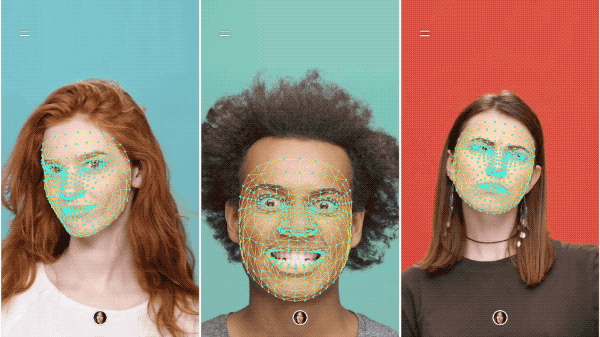
\includegraphics[width=0.7\textwidth]{Images/FaceRecognition.png}
     \caption[Detección de rostros]{Detección de rostros\footnotemark.}
     \label{fig:FaceRecognition}
 \end{figure}
  \footnotetext{Imagen sacada de  \url{https://ai.googleblog.com/2019/03/real-time-ar-self-expression-with.html}}
  
\subsubsection{Puntos de ancla(\textit{Anchor})}
Llamamos punto de anclaje o ancla, a un punto en el mundo real que se usa como referencia en el mundo virtual.\\

En la realidad aumentada tradicional el mecanismo utilizado para situar los objetos virtuales en el espacio real son los marcadores. La cámara identifica el patrón del marcador para  localizar la rotación y posición del objeto en cuestión. Sin embargo, en la realidad aumentada sin marcadores no disponemos de este sistema para guiarnos, de manera que tenemos que buscar otra forma de hacerlo.\\

Una vez localizado el plano o la superficie como explicábamos en secciones anteriores, las librerías de realidad aumentada sin marcadores son capaces de generar un objeto nulo cuya posición servirá como origen de coordenadas. Éste objeto es el llamado punto de ancla o \textit{anchor}, que servirá para colocar objetos virtuales en el mundo físico.\\

Para hacer un buen uso de ellos se debe evitar colocar puntos de anclado en superficies brillantes e intentar que la zona tenga una iluminación buena y consistente.

\subsubsection{Puntos de ancla en la nube (\textit{Cloud Anchor})}\label{cloudAnchorsSection}
El \textit{cloud anchor} es un mecanismo que permite colocar objetos virtuales en una escena de manera que múltiples usuarios puedan interactuar y ver los mismos objetos desde dispositivos distintos. Los objetos colocados pertenecen al mismo lugar físico independientemente del dispositivo que se use para verlo. Su funcionamiento es similar al de los puntos de ancla comunes, que se utilizan para fijar un objeto en una posición, con la diferencia de que los \textit{cloud anchors} se hospedan en los servidores en la nube. De esta manera varios dispositivos pueden consultarlos para situar los objetos en la aplicación.\\

Para ser utilizados, la aplicación en cuestión tiene que tener conexión a internet. Esta tecnología hoy en día sólo está implementada en las librerías ARCore y ARKit. El nombre de \textit{cloud anchors} son actualmente propios del SDK de ARCore, están soportados tanto en Android como en iOS (siempre que el dispositivo lo permita) y funcionan de la siguiente manera: la librería tiene que generar primero un mapa de las proximidades del punto de ancla que será el centro de interés. Para ello, la cámara recopila información y características del entorno cercano desde diferentes ángulos y posiciones durante unos segundos. Cuanto más precisa sea la información recopilada, mejor será la experiencia del usuario. Una vez transcurrido el tiempo, los parámetros del punto se hospedan en la nube y se establece el anchor, devolviendo el servidor un número de identificación único (el \textit{cloud anchor} ID). Cuando otro usuario de la aplicación dirige su cámara hacia el mismo punto de interés, el \textit{cloud anchor} procesa las características visuales del entorno físico desde el nuevo punto de vista. Estas características son comparadas con el mapa 3D que se ha generado anteriormente por el otro dispositivo y se establece la posición y orientación del nuevo usuario con respecto a ello para que pueda ver los objetos virtuales con la mayor precisión posible.\\

Para identificar un punto de ancla en la nube desde otro dispositivo se debe apuntar al lugar en que está situado sin importar la posición del dispositivo, siempre y cuando haya una línea recta entre ambos y no estén separados por una distancia superior a 10 metros.\\

En el caso de ARKit la tecnología para el usuario es igual, pero internamente no funciona de la misma manera. Por temas de privacidad, ARKit no manda los datos a un servidor, si no que utiliza el \textit{framework MultipeerConnectivity} de Apple para mandar la información del mapa (\textit{ARWorldMap}) por una conexión cliente a cliente~\cite{Apple_CloudAnchor}.\\

Cabe mencionar también que los \textit{cloud anchors} tienen una serie de limitaciones en el almacenamiento y el acceso a los datos. En el caso de Google, por ejemplo, sólo se puede acceder a ellos durante las 24 primeras horas después de haber sido colocados y 7 días después cualquier dato en la nube será borrado. El mapa hospedado en la nube no puede ser descargado por ningún usuario y no se puede determinar un lugar geográfico o reconstruir imágenes basándose en el mismo. Además, los datos que envía un dispositivo para que sean comparados con el mapa guardado no se almacenan nunca.\\

\section{Librerías de realidad aumentada sin marcadores}

En este apartado se describirán las principales librerías de realidad aumentada sin marcadores para más tarde estudiar las capacidades y posibilidades particulares de cada una de ellas en el apartado desarrollo.
Por cada librería se recogerán los siguientes datos:
\begin{itemize}
\item Breve descripción
\item Última versión
\item Funciones
\item Plataformas disponibles
\item Tipos de licencia
\end{itemize}
Luego se compararán todas entre sí para resumir las funcionalidades que tienen, las plataformas con las que son compatibles y los lenguajes que soportan.

\subsection{Wikitude}

Desarrollada por Wikitude GmbH, es una de las librerías pioneras en el mundo de la realidad aumentada. Lanzaron su primera aplicación en el 2008, desde entonces, son líderes del mercado. La versión que hemos usado ha sido Wikitude SDK 8.7.0 (2019-08-13)~\cite{Wikitude}.\\

Las principales funcionalidades son:
\begin{itemize}
\item Geo AR (Puntos de anclaje vía GPS)
\item Reconocimiento de imágenes 2D (marcadores) 
\item Reconocimiento de objetos 3D
\end{itemize}

Las plataformas móviles soportadas son:
\begin{itemize}
\item Android
\item iOS
\item Windows
\item Unity
\item Cordova
\item Xamarin
\item Flutter
\item Titanium
\end{itemize}
Soporte para Smart Glasses:
\begin{itemize}
\item Epson Moverio
\item Hololens
\item Vuzix
\end{itemize}
Otras plataformas:
\begin{itemize}
\item React Native
\item Ionic
\item Adobe Air
\item Qt by Felgo
\item LBAR
\end{itemize}
Licencias:
\begin{itemize}
\item SDK Startup. Gratuita para StartUps con menos de dos años de antigüedad y desarrolladores independientes que obtengan menos de 100.000\$ de beneficio en un año.
\item Wikitude Demo. Licencia de 30 días con marca de agua 499€
\item Wikitude SDK PRO (Sólo con marcadores y Geo AR). 1 año de licencia 1990€
\item Wikitude SDK PRO 3D (Paquete completo). 1 año de licencia 2490€
\end{itemize}

\subsection{ARKit}\label{ARKit_Sec}


Esta librería está desarrollada por Apple, fue presentada por primera vez en la Apple Worldwide Developers Conference de 2017.
La versión con la que trabajamos es la ARKit SDK 3.0~\cite{AppleDeve}. A diferencia del resto, para usar esta librería en Unity, no hace falta descargar ningún plugin, viene incluido en el paquete de Unity ARFoundation 2.2.\\

Funcionalidades:
\begin{itemize}
\item Reconocimiento de imágenes 2D (marcadores)
\item Reconocimiento de objetos 3D
\item Reconocimiento de rostro (hasta 3 simultáneamente)
\item Oclusión
\item SLAM
\item Estimación de luces
\item Puntos de anclaje en la nube
\end{itemize}
Las plataformas soportadas son:
\begin{itemize}
\item iOS 
\item Unity (via ARFoundation)
\item Unreal Engine 4~\cite{Unreal}
\end{itemize}
La licencia es gratuita.

\subsection{ARCore}\label{ARCore_Sec}


Esta librería está desarrollada por Google, y fue lanzada en febrero de 2018 como respuesta para competir contra ARKit de iOS. La versión con la que trabajamos es ARCore SDK for Unity v1.11.0 (2019-05-05)~\cite{ARCore}.\\

Funcionalidades:
\begin{itemize}
\item Reconocimiento de imágenes 2D (marcadores)
\item Reconocimiento de objetos 3D
\item Reconocimiento de rostro
\end{itemize}
\begin{itemize}
\item SLAM
\item Mapeado de áreas grandes
\item Estimación de luces
\item Puntos de anclaje en la nube
\end{itemize}
Las plataformas soportadas son:
\begin{itemize}
\item Android (Sólo los dispositivos soportados \cite{ARCoreList})
\item Android NDK
\item Unity (Android, iOS)
\item Unreal Engine 4
\item iOS
\end{itemize}
La licencia para usar ARCore es gratuita.


\subsection{Vuforia}

Esta librería está desarrollada por la empresa PTC. La versión que hemos utilizado ha sido Vuforia SDK Android 8.3.8 (2019-06-13)~\cite{Vuforia}.\\

Funcionalidades:
\begin{itemize}
\item Reconocimiento de imágenes 2D (marcadores)
\item Reconocimiento de objetos 3D
\item Escáner de objetos 3D
\end{itemize}
Plataformas:
\begin{itemize}
\item Android
\item iOS
\item Windows
\item Smart Glasses
\end{itemize}
Licencias:
\begin{itemize}
\item Básica, 42\$ al mes, limita el número de marcadores por licencia a 100.
\item Básica con base de datos en la nube para los marcadores 99\$ al mes.
\item Para la versión pro, la cual incluye marcadores ilimitados, acceso a API avanzada, y soporte en producción. Hay que contactar y hacen presupuesto a medida para la empresa.
\end{itemize}


\subsection{Kudan}


Kudan es una empresa que se dedica al desarrollo de la realidad aumentada, virtual y mixta, además de la conducción autónoma, drones y robots. La versión que hemos utilizado ha sido la Kudan SDK Unity 1.6.0 (2019-07-16)~\cite{Kudan}.\\

Funcionalidades:
\begin{itemize}
\item Reconocimiento de imágenes 2D (marcadores)
\item SLAM
\end{itemize}
Plataformas:
\begin{itemize}
\item Unity (Android, iOS)
\item iOS
\item Android
\end{itemize}
Licencias:
\begin{itemize}
\item AR Indie: Gratis. Pensado para la fase de desarrollo, protegido con marca de agua.
\item AR Business: 1500\$. Para las empresas con menos de un millón de dólares en ingresos.
\item AR Enterprise: Para las empresas con más de un millón de dólares en ingresos, hay que contactar con Kudan y proporcionan un presupuesto personalizado.
\end{itemize}


\subsection{MaxST}



Maxst se fundó en 2010 y se dedica a la investigación y desarrollo de la tecnología de realidad aumentada. Han lanzado Maxst AR SDK, el cual hemos probado en la versión MaxstARSDK\_Unity 4.1.3~\cite{Maxst}.\\

Funcionalidades:
\begin{itemize}
\item Reconocimiento de imágenes 2D (marcadores)
\item Reconocimiento de objetos 3D
\item Reconocimiento de códigos de barras y QR
\end{itemize}
Plataformas:
\begin{itemize}
\item Unity (Android,iOS)
\item Android
\item iOS
\item Windows
\item macOS
\item Epson Moverio BT-300,350 y ODG R-7
\end{itemize}
Licencias:

\begin{itemize}
\item Free. Gratis, para uso no comercial, incluye marca de agua.
\item Pro-one. Para aplicaciones con menos de 100k descargas (no incluye actualizaciones). Pago único de 499\$ 
\item Pro-Subscription. Subscripción anual, incluye actualizaciones 599\$ por año
\item Enterprise. Para aplicaciones con más de 100k de descargas. Hay que contactar con Maxst para recibir un presupuesto.
\end{itemize}


\subsection{8th Wall}


8th Wall desarrolla dos productos diferentes, 8th Wall Web y 8th Wall XR for Unity. El producto que vamos a analizar en el desarrollo es el 8th Wall XR for Unity 11.2.6.519, para que la comparación entre las librerías sea mas precisa, ya que la potencia que tiene en navegador es menor a la que puede llegar a tener una aplicación de Unity~\cite{8thWall}.\\

Funcionalidades:
\begin{itemize}
\item Reconocimiento de imágenes 2D (marcadores)
\item 6 grados de libertad
\item SLAM
\item Estimación de la luz
\end{itemize}

Plataformas:
\begin{itemize}
\item Unity (Android, iOS)
\item Web (A-Frame, BabylonJS, Sumerian, three.js) soportada en la versión web
\end{itemize}
El uso de 8th Wall XR de Unity es gratuito. En el caso de 8th Wall Web, la licencia se cobra según las visitas en la web. Aparte, se necesita una licencia de desarrollador que cuesta 250\$/mes.\\

\begin{table}[H]
    \centering
    \begin{tabular}{c c c c}
    \toprule
        Pago por visita (PPV)&	Paquete estándar&PPV de alto tráfico&Paquete alto tráfico \\
         \midrule
        1000\$/mes	& 3000\$/mes	& 6000\$/mes &	6000\$/mes \\  
 
        0 visitas incluidas &	500k visitas incluidas&	0 visitas incluidas	&5M visitas incluidas\\
 
        0.01\$/visita&	0.01\$/visita extra&	0.0025\$/visita&	0.0025\$/visita extra\\
      \bottomrule
    \end{tabular}
    \caption{Licencias 8th Wall}
    \label{tab:8thwallLicenses}
\end{table}


\\

\subsection{Easy AR}


EasyAR es una compañía china que lleva en el mercado desde 2016. Hemos probado la versión EasyARSense Unity SDK v3.0.1(2019-07-07)~\cite{EasyAR}.\\

Funcionalidades:
\begin{itemize}
\item Reconocimiento de imágenes 2D (marcadores)
\item Reconocimiento de objetos 3D
\item SLAM
\item Grabación de pantalla
\end{itemize}
Plataformas soportadas:
\begin{itemize}
\item Unity (Android, iOS)
\item Android
\item iOS
\item Windows
\end{itemize}
Licencias:
\begin{itemize}
\item EasyAR SDK Basic. Gratis
\item EasyAR SDK Pro, 499\$ por licencia. Añade el reconocimiento de objetos 3D, la grabación de pantalla y reconocimiento de más de un marcador simultáneo.
\item EasyAR SDK Pro trial. Lo mismo que el Pro, pero limitado a 100 usos por día.
\end{itemize}


\subsection{ARFoundation}


Este último no se trata exactamente de una librería, sino de un paquete de Unity (aún en fase experimental) que integra una API de alto nivel (wrapper) que permite tener el mismo código funcional para ARCore y ARKit, según si se compila el proyecto para Android o para iOS. La versión más reciente es ARFoundation 2.2 (Unity 2019.1), incluye las versiones más recientes de ambas librerías~\cite{ARFoundation}.\\

Soporta las mismas funcionalidades que ARCore y ARKit:
\begin{itemize}
\item Reconocimiento de imágenes 2D (marcadores)
\item Reconocimiento de objetos 3D
\item Reconocimiento de rostro 
\item Oclusión (iOS con ARKit)
\item SLAM
\item Mapeado de áreas grandes (ARCore)
\item Estimación de luces
\item Puntos de anclaje en la nube
\end{itemize}

Plataformas soportadas:
\begin{itemize}
\item Unity (Android, iOS)
\end{itemize}

Su licencia, al igual que ARCore y ARKit, es gratuita.
\section{Resumen de características}
\subsection{Tabla de funcionalidades}
A continuación, en la tabla \ref{tab:funcionalidades} se puede ver un resumen de  las funcionalidades que tiene cada una de las librerías que vamos a analizar. Más adelante, en la parte de comparación y análisis de las librerías, evaluaremos la calidad y eficiencia de estas funcionalidades para cada librería.

\begin{table}[H]
\resizebox{\textwidth}{!} {
    \centering
    \begin{tabular}{m{2cm} c c m{2cm} c c c m{2cm}}
    \toprule
        SDK & Marcadores 2D & Marcadores 3D & Tipo tracking & SLAM & Detección de rostro & Estimación de luces & Otras \\
\midrule
\textbf{Wikitude} & \checkmark & \checkmark & Tracking instantáneo & \checkmark & - & \checkmark & Geo AR \\

\textbf{ARKit} & \checkmark & \checkmark & Detección de planos & \checkmark & \checkmark & \checkmark & Oclusión, Cloud Anchor \\

\textbf{ARCore} & \checkmark & \checkmark & Detección de planos & \checkmark & \checkmark & \checkmark & Cloud Anchor \\

\textbf{Vuforia} & \checkmark & \checkmark & Detección de planos & \checkmark & – & \checkmark &  \\

\textbf{Kudan} & \checkmark & - & Tracking instantáneo & \checkmark & - & \checkmark &  \\

\textbf{MaxST} & \checkmark & \checkmark & Tracking instantáneo & \checkmark & – & \checkmark & \\

\textbf{8th Wall XR} & \checkmark & – & Detección de planos & \checkmark & – & \checkmark &  \\

\textbf{EasyAR} & \checkmark & \checkmark & Tracking instantáneo & \checkmark & – & \checkmark & Grabación de pantalla \\

\textbf{AR Foundation} & \checkmark & \checkmark & Detección de planos & \checkmark & \checkmark & \checkmark & \\
\bottomrule
    \end{tabular}
  }
    \caption{Comparación de funcionalidades}
    \label{tab:funcionalidades}
\end{table}
Como vemos en la tabla~\ref{tab:funcionalidades}, menos en el reconocimiento de rostro, casi todas las librerías tienen las mismas funcionalidades, por lo que a priori nos sirve cualquiera para realizar nuestras pruebas de concepto. Por lo que se probarán todas y se verán cuáles son las que mejor resultado proporcionan.

\subsection{Lenguajes y plataformas soportados}

Podemos ver en la tabla~\ref{tab:plataformas} que prácticamente todas las librerías soportan Android e iOS, con lo que podemos deducir que es donde más se está invirtiendo en el mercado. Quizás las \textit{smartglasses} puedan brindar una experiencia de realidad aumentada más agradable, pero todavía está muy lejos de ser accesible para la mayoría de la población, mientras que un dispositivo móvil es mucho más asequible.

\begin{table}[H]
\resizebox{\textwidth}{!} {
    \centering
    \begin{tabular}{c c c c c c c c}
    \toprule
       SDK &	Unity3D (Android, iOS) &	Unreal Engine 4 &	Java &	Objective-C &	C++ & JavaScript \\
       \midrule
Wikitude & \checkmark & – & \checkmark & \checkmark & – & \checkmark \\

ARKit & \checkmark & \checkmark & – & \checkmark & – & – \\

ARCore & \checkmark & \checkmark & \checkmark & \checkmark & – & – \\

Vuforia & \checkmark & – & \checkmark & \checkmark & \checkmark & – \\

Kudan & \checkmark & – & \checkmark & \checkmark & – & – \\

MaxST & \checkmark & – & \checkmark & – & \checkmark & – \\

8th Wall  & \checkmark & – & – & – & – & \checkmark \\

EasyAR & \checkmark & – & \checkmark & \checkmark & \checkmark & – \\

AR Foundation & \checkmark & – & – & – & – & – \\
\bottomrule
    \end{tabular}
  }
    \caption{Comparación de plataformas y lenguajes soportados}
    \label{tab:plataformas}
\end{table}

En la tabla \ref{tab:plataformas}, es muy fácil observar que Unity3D sale ganador, se puede trabajar con absolutamente todas las librerías, además gracias a su editor y entorno visual, resulta muchísimo más cómodo y ahorra mucho tiempo a la hora de desarrollar una aplicación de realidad aumentada.\\

Después de haber analizado las características de éstas librerías de realidad aumentada, en el siguiente capítulo sometemos a cada librería a una prueba para evaluar su funcionamiento.

\section*{Resumen}
Existen diferentes formas de seguimiento en la realidad aumentada: utilizando marcadores, no utilizándolos y basándose en la geolocalización. Estos tipos de seguimiento pueden funcionar de dos maneras. La forma \textit{Bottom-Up} busca calcular la posición del dispositivo en relación a la información que obtiene de la cámara. Esta información puede venir en forma de marcadores físicos, planos, patrones faciales, etc. Por otro lado, la forma \textit{Top-Down} hace una estimación inicial de la posición de la cámara y después con la información que recibe corrige la aproximación previa.\\

En la realidad aumentada sin marcadores se utilizan una serie de tecnologías para calcular la posición de la cámara y los objetos virtuales en la escena física. Algunos de estos métodos son: SLAM, reconocimiento del ambiente, detección de oclusión, detección de rostros y puntos de anclaje.\\

En este capítulo hemos dado un vistazo rápido a las características principales de las librerías de realidad aumentada sin marcadores. En el siguiente capítulo profundizaremos más en el funcionamiento de cada una y las evaluaremos de acuerdo a las pruebas que hemos realizado.

\noindent

\chapter{Comparación y análisis de las librerías}

El análisis de las librerías se estructurará en los puntos que se describen a continuación:
\begin{itemize}
\item Calidad de la documentación y primeros pasos: en este punto evaluaremos la dificultad para realizar una aplicación básica con cada librería, desde el momento en el que se descarga el SDK, hasta que se construye la APK. 
\item Evaluación de las capacidades de la librería: en este apartado se tendrán en cuenta las funcionalidades, las tecnologías que soporta y el nivel personalización dentro de la App, es decir, hasta que nivel podemos usar la API que nos proporcionan.
\item Conclusiones: gracias al estudio realizado estableceremos unas conclusiones sobre el uso de cada librería y decidiremos si nos facilita el desarrollo de alguna prueba de concepto.
\end{itemize}


Para realizar la evaluación de las capacidades y los límites de cada librería se realizará un test que consistirá en:
\begin{itemize}
\item Instanciar un objeto.
\item Movernos alrededor de dicho objeto, para comprobar la estabilidad del punto de anclaje.
\item Realizar movimientos bruscos y veloces para ver si pierde la referencia en algún momento.
\item Hacer que pierda la referencia y comprobar el tiempo en el que vuelve a aparecer el objeto.
\item Alejarnos del objeto y ver hasta que distancia sigue funcionando.
\item Comprobar cómo se comportan las librerías con diferentes intensidades de luz.
\end{itemize}
Los vídeos se encuentran aquí: \url{ https://www.youtube.com/playlist?list=PLqQgTAUiabc8AQrcc48Jdglnytus9IoXe}
\clearpage
\section{Wikitude}

\subsection{Calidad de la documentación y primeros pasos}
La experiencia al crear una aplicación usando Wikitude es buena. Te guían desde el momento en el que entras a la web, a descargar el SDK que necesites, eso sí, hace falta registrarse y para que funcione la aplicación hay que descargar una clave de licencia, la cual hay que introducir en el componente Wikitude Camera que trae el paquete. Todos estos pasos vienen documentados, y para facilitar el proceso de prueba, traen varias escenas montadas en las que se pueden probar diferentes tipos de tecnologías. Para hacer funcionar todas las escenas, es necesario que el \textit{Package Name} de la aplicación sea ``com.wikitude.unityexample'', ya que el SDK está protegido de esta manera. La documentación de la API es muy completa y está muy bien estructurada.\cite{WikitudeDoc}
\subsection{Evaluación de las capacidades de la librería}
\textbf{Condiciones de luz mínimas:}\\
\textbf{Esta prueba está disponible en el link:} \url{https://youtu.be/_4fLQas1NcM}\\

La sala está únicamente iluminada por un haz de luz perteneciente a una habitación situada al otro lado del pasillo.\\

Consigue instanciar el objeto dentro de un plano y posee buena iluminación. El plano falla cuando empezamos a movernos haciendo un giro de 45º no esperado, si estamos encima del modelo se pierde, si damos la vuelta completa sigue perdido. Necesitamos volver a referenciarlo por que no se recupera. La calidad del modelo y su textura es óptima para las condiciones de luz que posee. Se pierde la referencia fácilmente ante los giros. Cuando se realiza un movimiento de cámara en el que el punto de anclaje sale del \textit{frustrum}\footnote{Región cerrada del espacio que delimita los objetos que aparecen representados en la pantalla.}  y más tarde se vuelve a enfocar a él, tarda un segundo en volver a posicionar el plano y su objeto. En esta primera prueba no hemos conseguido que pierda la referencia por distancia, se repetirá con un escenario más amplio. Hace estimaciones con oclusión desapareciendo con la pared.\\

\textbf{Condiciones de luz ambiente:}

\textbf{Esta prueba está disponible en el link:} \url{https://youtu.be/wlqITlPTz3o}\\

La sala está únicamente iluminada por dos ventanas a la luz de la tarde.\\

Consigue instanciar el objeto dentro de un plano y posee buena iluminación. El plano falla cuando empezamos a movernos haciendo de nuevo un giro de 45º no esperado, si estamos encima del modelo se pierde pero en este caso se recupera con cierta facilidad. Podemos acercarnos bastante manteniendo el nivel de detalle. La calidad del modelo y su textura es óptima para las condiciones de luz que posee. Se pierde la referencia fácilmente ante los giros. Cuando se realiza un movimiento de cámara en el que el punto de anclaje sale del \textit{frustrum} y más tarde se vuelve a enfocar a él, tarda menos de un segundo en volver a posicionar el plano y su objeto. En esta primera prueba no hemos conseguido que pierda la referencia por distancia. Hace estimaciones con oclusión desapareciendo con la pared.

\begin{table}[H]
    \centering
    \begin{tabular}{|l|c|c|}
    \hline
          & Luz Ambiente & Luz Mínimas \\
         \hline
        Estabilidad del punto de anclaje   &4 &6\\
        \hline
        Estimación y calidad de iluminación  &7 &8 \\
        \hline
        Resistencia a movimientos  &1 &2 \\
        \hline
        Recuperación del ancla  &8 &8 \\
      \hline
    \end{tabular}
    \caption{Análisis Wikitude}
    \label{tab:TWikitude}
\end{table}

\subsection{Conclusiones}

\clearpage
\section{ARKit}
\subsection{Calidad de la documentación y primeros pasos}

\subsection{Evaluación de las capacidades de la librería}

\subsubsection{Condiciones de luz mínimas:}

\textbf{Esta prueba está disponible en el link:} \url{https://youtu.be/uwjq-bF_J4M}\\

La sala está únicamente iluminada por un haz de luz perteneciente a una habitación situada al otro lado del pasillo y una pequeña iluminación frontal.

Necesita significativamente más luz(2) para reconocer el plano, en parte debido al dispositivo. La estimación de la iluminación es excelente como podemos ver a lo largo de la prueba. Al realizar un movimiento alrededor del modelo no se pierde ni se desestabiliza en ningún momento. Al posicionar el teléfono sobre el modelo sigue estable. Las texturas del modelo se ven de manera nítida y realista. En la prueba de resistencia a movimientos bruscos se desplaza el plano en ocasiones recuperándose en un breve periodo de tiempo (menor a un segundo). Cuando se realiza un movimiento en el que el modelo desaparece del campo de visión este no llega a desaparecer nunca del entorno virtual por lo que al volver a enfocar al punto de anclaje la transición es limpia.

\subsubsection{Condiciones de luz ambiente:\\}

\textbf{Esta prueba está disponible en el link:} \url{https://youtu.be/zcm59hRtJeQ}\\

La sala está únicamente iluminada por dos ventanas a la luz de la tarde.\\
Reconoce los planos de casi instantáneamente, por lo que nos permite posicionar el objeto sin esperas. La calidad de las texturas son muy buenas y la estimación de luz es impresionante, la luz cambia mientras rodeamos al modelo, estando mas oscuro cuando nos encontramos a contraluz, e iluminado nos situamos entre la luz entrante y el modelo. La estabilidad del objeto es sobresaliente, nos permite rodear el objeto y acercarnos todo lo posible sin que se mueva. La resistencia a movimientos bruscos funciona muy bien, situando al modelo siempre en su punto origen. Lo mismo ocurre en la prueba de sacar el punto de anclaje del campo de visión de la cámara,el dragón nunca desaparece, por lo que al volver a enfocar el punto de partida, vemos una transición muy natural.


\begin{table}[H]
    \centering
     \begin{tabular}{|l|c|c|}
    \hline
          & Luz Ambiente & Luz Mínimas \\
         \hline
        Estabilidad del punto de anclaje   &4 &6\\
        \hline
        Estimación y calidad de iluminación  &7 &8 \\
        \hline
        Resistencia a movimientos  &1 &2 \\
        \hline
        Recuperación del ancla  &8 &8 \\
      \hline
    \end{tabular}
    \caption{Análisis ARKit}
    \label{tab:TARKit}
\end{table}

\subsection{Conclusiones}
Como hemos comprobado anteriormente, en unas condiciones de luz mínimas el trabajo de esta librería ha sido casi excelente. Su único fallo era la resistencia a movimientos bruscos, la cual se arregla cuando las condiciones lumínicas son óptimas, pudiendo disfrutar de una experiencia perfecta. Si ya con la luz mínima era casi perfecta, con unas condiciones buenas de luz, estamos ante una de las mejores opciones a la hora de crear una experiencia de realidad aumentada. Cabe destacar que ARKit sólo está soportado en dispositivos iOS, por lo que se puede controlar mucho más el abanico de dispositivos en el que se va a usar la aplicación. Lo cual es útil a la hora de asegurar el correcto funcionamiento de las aplicaciones.

\clearpage
\section{ARCore}
\subsection{Calidad de la documentación y primeros pasos}
Hacer funcionar una aplicación con ARCore es tan fácil como descargar el SDK desde su Github oficial \cite{Github_Google}, añadir una de las escenas de ejemplo a la build, seleccionar dentro de Unity3D la opción de ``Player Settings -> XR Settings -> ARCore Supported''.Para probar la realidad aumentada con ARCore no hace falta registrarse ni obtener ninguna licencia para que funcione, exceptuando el uso de los \textit{Cloud Anchors}, en el siguiente capítulo explicaremos cómo activarlos. La documentación de los pasos a seguir y de la API es bastante completa, además es de que al ser una de las librerías más usadas en la comunidad, hay muchos tutoriales en el que puedes aprender sobre ella. Para facilitar el desarrollo de aplicaciones con ARCore, Google ha desarrollado una aplicación \textit{ARCore Instant Preview}, la cual se engancha vía USB o Wifi con el editor de Unity3D, y permite probar las aplicaciones en el teléfono sin necesidad de generar una APK.
\subsection{Evaluación de las capacidades de la librería}
\subsubsection{Condiciones de luz mínimas:}\\
\textbf{Esta prueba está disponible en el link:} \url{https://youtu.be/uSRztU8z18U}\\
La sala está únicamente iluminada por un haz de luz perteneciente a una habitación situada al otro lado del pasillo y una pequeña iluminación frontal.\\

Necesita más luz(2) para reconocer el plano. La estimación de la iluminación es excelente como podemos ver a lo largo de la prueba. Al realizar un movimiento alrededor del modelo no se pierde ni se desestabiliza en ningún momento. Al posicionar el teléfono sobre el modelo sigue estable. Las texturas del modelo se ven de manera nítida y realista. En la prueba de resistencia a movimientos bruscos no desaparece nunca ni vibra la imagen dando unos resultados óptimos. Cuando se realiza un movimiento en el que el modelo desaparece del campo de visión este no llega a desaparecer nunca del entorno virtual por lo que al volver a enfocar al punto de anclaje la transición es limpia.

\subsubsection{Condiciones de luz ambiente:}

\textbf{Esta prueba está disponible en el link:} \url{https://youtu.be/PLXAEFJn4rQ}\\

En este caso reconoce los planos al instante gracias a las condiciones lumínicas. La estimación de la iluminación es sorprendente, ya que mientras giramos alrededor del modelo la luz reacciona a nuestros movimientos. Podemos observar que al posicionarnos en contraluz el objeto está menos iluminado que al comienzo de la prueba donde la luz era directa. En el segundo caso creemos que la intensidad de la luz estimada es un poco excesiva. Los movimientos de cámara se mantienen como en la primera prueba teniendo un resultado perfecto.

\begin{table}[H]
    \centering
      \begin{tabular}{|l|c|c|}
    \hline
          & Luz Ambiente & Luz Mínimas \\
         \hline
        Estabilidad del punto de anclaje   &10 &10\\
        \hline
        Estimación y calidad de iluminación  &8 &9 \\
        \hline
        Resistencia a movimientos  &10 &10 \\
        \hline
        Recuperación del ancla  &10 &10 \\
      \hline
    \end{tabular}
    \caption{Análisis ARCore}
    \label{tab:TARCore}
\end{table}
\subsection{Conclusiones}
Los resultados obtenidos con ARCore han sido magníficos, el único punto flojo es cuando las condiciones de luz son muy bajas, porque no es capaz de detectar la superficie. Quitando esa situación, la experiencia obtenida es muy buena, porque es muy estable y además la estimación de luz funciona casi a la perfección. Como hemos comentado antes, hay situaciones en las que es exagerado el brillo que obtiene. A pesar de sus resultados, también tiene una parte mala, su lista de dispositivos soportados \cite{ARCoreList}. Aunque con el paso del tiempo esa lista va creciendo y los móviles nuevos cada vez son más potentes, aun queda mucho porcentaje de dispositivos que no están soportados, por lo que el público al que puede llegar una aplicación de realidad aumentada usando ARCore es limitado.

\clearpage
\section{Vuforia}
\subsection{Calidad de la documentación y primeros pasos}
Los primeros pasos con esta librería en Unity son muy accesibles, gracias a una documentación de calidad podemos ser guiados paso a paso para la creación de una nueva experiencia de realidad aumentada. La integración con Unity es muy 


\subsection{Evaluación de las capacidades de la librería}
\subsubsection{Condiciones de luz mínimas:}

\textbf{Esta prueba está disponible en el link:} \url{https://youtu.be/4Y_Enzrx17w}

La sala está únicamente iluminada por un haz de luz perteneciente a una habitación situada al otro lado del pasillo y una iluminación frontal.\\

El nivel de luz de la sala no supone ningún problema para posicionar el modelo. La calidad de las texturas del objeto son malas, además no existe ninguna estimación de iluminación sobre el modelo. El anclaje alrededor del objeto con movimientos suaves es malo ya que se mueve con nosotros. La estabilidad del objeto cuando nos movemos en sus proximidades es mala ya que el objeto cambia de posición a medida que nos acercamos. No conseguimos perder el objeto con la distancia. La capacidad de soportar movimientos bruscos es buena, ya que no pierde la posición del ancla. Al sacarlo del campo de visión lo mantiene en su posición en todo momento.

\subsubsection{Condiciones de luz ambiente:\\}

\textbf{Esta prueba está disponible en el link:} \url{https://youtu.be/zlUj-jh7Uts}

Después de mejorar las condiciones de luz se mantienen los problemas de estimación de luz. La visualización del modelo renderiza las texturas de manera muy pobre siendo muy poco realista. La estabilidad del objeto mejora ya que podemos girar alrededor del objeto sin perder la referencia, permitiéndonos acercarnos en esta ocasión. Se mantiene la capacidad de soportar movimientos bruscos y la robustos en cuanto al campo de visión.

\begin{table}[H]
    \centering
     \begin{tabular}{|l|c|c|}
    \hline
          & Luz Ambiente & Luz Mínimas \\
         \hline
        Estabilidad del punto de anclaje   &4 &6\\
        \hline
        Estimación y calidad de iluminación  &7 &8 \\
        \hline
        Resistencia a movimientos  &1 &2 \\
        \hline
        Recuperación del ancla  &8 &8 \\
      \hline
    \end{tabular}
    \caption{Análisis Vuforia}
    \label{tab:TVuforia}
\end{table}
\subsection{Conclusiones}

\clearpage
\section{Kudan}
\subsection{Calidad de la documentación y primeros pasos}
Los primeros pasos con Kudan no son tan gratificantes en comparación a sus competidores. Empezando por la descarga del SDK, ésta ni si quiera se encuentra en la página oficial \cite{Kudan_Official}, si no que se encuentra en XLSoft \cite{Kudan}. Una vez metido el SDK en Unity, en las carpetas vienen escenas de ejemplo, en las que podemos ver como se monta una aplicación con Kudan. La librería está protegida por \textit{Package Name}, contactando con los desarrolladores de Kudan puedes obtener una clave de licencia para cualquier \textit{Package Name}, sin embargo, proporcionan una general con la que podemos desarrollar ``com.xlsoft.kudanar''. \cite{Kudan_License}La documentación para los primeros pasos es aceptable, pero sobre el SDK y la API no hay documentación, únicamente los comentarios en los scripts. Una vez instalada la aplicación en el teléfono, seguramente no funcione ya que la aplicación no pide los permisos para usar la cámara, y sin ellos Kudan no puede inicializarse. Para arreglar este error, hace falta añadir en algún script esta línea de código "Permision.RequestUserPermission(Permission.Camera)'', que se encuentra en el paquete "UnityEngine.Android''.
\subsection{Evaluación de las capacidades de la librería}\\
\subsubsection{Condiciones de luz mínimas:}

\textbf{Esta prueba está disponible en el link:}\url{https://youtu.be/cLJMyV9bV6s}

La sala está únicamente iluminada por un haz de luz perteneciente a una habitación situada al otro lado del pasillo.\\

El nivel de luz de la sala no supone ningún problema para posicionar el modelo. La calidad de las texturas del objeto son malas, además no existe ninguna estimación de iluminación sobre el modelo. El anclaje alrededor del objeto con movimientos suaves es aceptable pero en el momento que nos acercamos se pierde y hay que volver a referenciarlo. La estabilidad del objeto cuando nos movemos en sus proximidades es muy mala, cambiando de tamaño sin sentido aparente. La distancia máxima de captura es de siete metros aproximadamente. La capacidad de soportar movimientos bruscos es mala, pierde totalmente la posición del ancla con resultados incorrectos e incluso a veces pierde la referencia del todo. Al sacarlo del campo de visión no lo posiciona en el mismo punto donde estaba, llegando a perder en ocasiones el punto de referencia.

\subsubsection{Condiciones de luz ambiente:}

\textbf{Esta prueba está disponible en el link:}\url{https://youtu.be/JyjBmQZZ5E4}

Gracias a las condiciones de luz la estabilidad del objeto en la escena mejora sustancialmente, pudiendo dar la vuelta casi perfecta al objeto sin problemas, exceptuando la posición cenital que genera desestabilización breve en el objeto. Se mantiene la distancia máxima de siete metros. Además en esta ocasión la resistencia ante movimientos bruscos mejora considerablemente, sin llegar a ser correcta ya que pierde la referencia en una ocasión. En el caso del campo de visión recupera el objeto de manera más óptima sin llegar a volver a posicionar con precisión el objeto.

\begin{table}[H]
    \centering
     \begin{tabular}{|l|c|c|}
    \hline
          & Luz Ambiente & Luz Mínimas \\
         \hline
        Estabilidad del punto de anclaje   &3 &6\\
        \hline
        Estimación y calidad de iluminación  &0 &0 \\
        \hline
        Resistencia a movimientos  &2 &7 \\
        \hline
        Recuperación del ancla  &3 &6 \\
      \hline
    \end{tabular}
  
    \caption{Análisis Kudan}
    \label{tab:TKudan}
\end{table}
\subsection{Conclusiones}
Los resultados obtenidos con Kudan no son muy buenos, además de que no renderiza la cámara en la aplicación, por lo que se ve con un fondo negro, impidiendo que la experiencia sea tan inmersiva frente a las demás librerías. Los resultados con condiciones de luz mínimas han sido muy malos, y aunque cuando hemos aumentado la cantidad de luz ha mejorado bastante, no llega al nivel de los competidores.
\clearpage
\section{Maxst}
\subsection{Calidad de la documentación y primeros pasos}
Para usar Maxst, hace falta registrarse en su página web \cite{Maxst}, y acceder a la descarga del SDK. Además, hay que generar una clave de licencia específica para nuestro \textit{Package Name}.La documentación  es buena en ambos casos, en la guía de integración y de la API. Una vez importado la librería en Unity, se puede ver que hay escenas de ejemplo ya hechas, por lo que simplemente hay que añadirlas a la \textit{Build} de la aplicación. Se pueden probar las aplicaciones también desde el editor, usando una cámara que esté conectada al ordenador, obviamente funciona peor que en un móvil, ya que la cámara no tiene sensores, pero sirve para darnos una idea del tamaño de los objetos. 
\subsection{Evaluación de las capacidades de la librería}
\subsubsection{Condiciones de luz mínimas:}

\textbf{Esta prueba está disponible en el link:}\url{https://youtu.be/QFX_B8HX1yU}

La sala está únicamente iluminada por un haz de luz perteneciente a una habitación situada al otro lado del pasillo.\\

El nivel de luz de la sala no supone ningún problema para posicionar el modelo. La calidad de las texturas del objeto son notables, no existe ninguna estimación de iluminación sobre el modelo. El anclaje alrededor del objeto con movimientos suaves es aceptable pero en el momento que nos acercamos se pierde y no se llega a recuperar el punto teniendo que volver a referenciarlo.  No somos capaces de dar la vuelta al modelo completo sin perderlo. No conseguimos perderlo con la distancia. La capacidad de soportar movimientos bruscos es mejorable ya que no desaparece el modelo, pero si pierde su referencia en el espacio moviéndolo a una posición diferente. Al sacarlo del campo de visión no lo posiciona de nuevo en la mayoría de las ocasiones. Sin embargo, cuando consigue mantenerlo, en la mayoría de ocasiones se desplaza del punto correcto y muy rara vez muestra la opción correcta.

\subsubsection{Condiciones de luz ambiente:}

\textbf{Esta prueba está disponible en el link:}\url{https://youtu.be/cspBAaQCfew}

La estabilidad a mejorado notablemente, permitiendo dar la vuelta completa. En ocasiones pierde la referencia y se desplaza el modelo un poco si nos acercamos demasiado. Si pierdes el punto de visión por ejemplo cruzando una pared desaparece el modelo, pero si volvemos al punto de partida es capaz de recuperar la referencia en aproximadamente 7 segundos. La resistencia a los giros bruscos ha mejorado muy considerablemente llegando a ser casi perfecta, a veces se desplaza en algún fotograma pero se reposiciona rápidamente. Al sacar el modelo del campo de visión de la cámara y luego volver a meterlo rinde mejor con el entorno iluminado, consiguiendo que esté bien posicionado, eso sí, a veces sigue desapareciendo y volviendo a aparecer, impidiendo así una transición limpia.

\begin{table}[H]
    \centering
      \begin{tabular}{|l|c|c|}
    \hline
          & Luz Ambiente & Luz Mínimas \\
         \hline
        Estabilidad del punto de anclaje   &4 &6\\
        \hline
        Estimación y calidad de iluminación  &1 &1 \\
        \hline
        Resistencia a movimientos  &4 &9 \\
        \hline
        Recuperación del ancla  &3 &7 \\
      \hline
    \end{tabular}
    \caption{Análisis Maxst}
    \label{tab:TMaxst}
\end{table}
\subsection{Conclusiones}
Apenas necesita tiempo para posicionar el ancla, no hay que esperar a que reconozca una superficie plana, pero la estabilidad debe mejorar un poco. A pesar de que al estar en unas condiciones lumínicas ideales, el modelo a veces se mueve cuando estamos muy cerca e incluso puede llegar a perderse la referencia. Esto es crítico si se quiere desarrollar una aplicación en la que se pueda mover alrededor de un punto, o acercarse mucho a él para poder verlo con detalle. 
\clearpage
\section{8th Wall XR}
\subsection{Calidad de la documentación y primeros pasos}
Para desarrollar aplicaciones de realidad aumentada con 8thWall, es necesario registrarse en su página web \cite{8thWall}, descargar el SDK, y generar una clave de licencia, que tendremos que especificar en el objeto ``XRAppSettings'' que se encuentra dentro del paquete de Unity3D. Estos pasos vienen bien documentados en la guía que proporcionan, por lo que la calidad de la documentación es buena, también en la parte de la API. Tienen tutoriales subidos en los que enseñan y explican cómo desarollar aplicaciones con su SDK. En los dispositivos que se encuentran en la lista de ARCore \cite{ARCoreList}, 8thWall usa ARCore para la tecnología de realidad aumentada. Para los que no se encuentran en esa lista, tienen su propia tecnología, que no funciona tan bien,pero por lo menos permite cubrir un rango muy amplio de dispositivos soportados. Para facilitar el desarrollo, han creado una aplicación para probar en el móvil desde el editor de Unity3D, llamada \textit{8th Wall XR Remote}, que se puede encontrar en \textit{Google Play} \cite{8thWallRemote}.
\subsection{Evaluación de las capacidades de la librería}
\subsubsection{Condiciones de luz mínimas:}\\
\textbf{Esta prueba está disponible en el link:}\url{https://youtu.be/6edM5PhhXj0}\\
La sala está únicamente iluminada por un haz de luz perteneciente a una habitación situada al otro lado del pasillo.\\

El nivel de luz de la sala supone un problema para posicionar el modelo con lo que aumentamos el nivel de luz. La calidad de las texturas del objeto son buenas, además posee estimación de iluminación sobre el modelo correcta y muy eficaz. El anclaje alrededor del objeto con movimientos suaves es muy buena pudiendo dar una vuelta sin problema y acercarnos para ver el detalle del dragón sin que desaparezca. No conseguimos perderlo con la distancia en ningún momento. La capacidad de soportar movimientos bruscos es muy resistente, nunca se pierde y su anclaje sigue en la posición correcta. Al sacarlo del campo de visión lo mantiene creando una transición suave. 

\subsubsection{Condiciones de luz ambiente:}\\
\textbf{Esta prueba está disponible en el link:}\url{https://youtu.be/5TBd3ml35RY}\\

La detección del plano es muy rápida. Mantiene y mejora la calidad de las texturas del objeto, así como la estimación de iluminación. El anclaje alrededor del objeto con movimientos suaves es muy buena pudiendo dar una vuelta sin problema y acercarnos para ver el detalle del dragón sin que desaparezca. No conseguimos perderlo con la distancia en ningún momento. La capacidad de soportar movimientos bruscos y movimientos fuera del campo de visión continua siendo muy resistente.

\begin{table}[H]
    \centering
      \begin{tabular}{|l|c|c|}
    \hline
          & Luz Ambiente & Luz Mínimas \\
         \hline
        Estabilidad del punto de anclaje   &10 &10\\
        \hline
        Estimación y calidad de iluminación  &8 &8 \\
        \hline
        Resistencia a movimientos  &10 &10 \\
        \hline
        Recuperación del ancla  &10 &10 \\
      \hline
    \end{tabular}
    \caption{Análisis 8th Wall}
    \label{tab:T8thWall}
\end{table}
\subsection{Conclusiones}
Aunque por debajo utilice la misma tecnología que ARCore, la capa que han desarrollado por encima simplifica bastante el uso de la librería y el desarrollo de una aplicación con realidad aumentada. Por esta razón, y por los resultados obtenidos, que han sido excelentes, esta librería una muy buena opción para desarrollar una aplicación. Además, el otro producto que desarrolla la empresa, 8th Wall for Web, permite llevar la realidad aumentada a un navegador de manera muy sencilla, sin necesidad de instalar una aplicación completa. Aunque los resultados no son tan buenos, se defiende muy bien \cite{8thWallJini}.
\clearpage
\section{Easy AR}
\subsection{Calidad de la documentación y primeros pasos}
Es necesario registrarse para acceder a la descarga del SDK y generar una clave de licencia. Una vez importado el paquete dentro de Unity, hay que buscar el objeto ``EasyARKey'' y especificar la clave. Las escenas que vienen de ejemplo no son del todo intuitivas ni modificables, ya que para cambiar el objeto que se instancia hay que entrar y hacer unos cambios en el código, lo ideal sería poder cambiarlo desde el editor. La documentación es mejorable, solo tienen una guía para hacer la \textit{Build} en cada plataforma, pero no hay ninguna guía que explique como crear una aplicación desde cero, ni explican cuales son las clases y componentes importantes e inprescindibles.

\subsection{Evaluación de las capacidades de la librería}
\subsubsection{Condiciones de luz mínimas:}\\
\textbf{Esta prueba está disponible en el link:}\url{https://youtu.be/G_iY6gdoMOU}\\

La sala está únicamente iluminada por un haz de luz perteneciente a una habitación situada al otro lado del pasillo.\\

Coloca el modelo enfrente del usuario automáticamente sin buscar ningún plano de referencia. La estabilidad del objeto es muy mala ya que no nos podemos acercar porque el objeto también se mueve con el usuario, lo mismo ocurre al intentar dar la vuelta sobre él. La calidad de texturas es aceptable y no posee estimación de luz. La resistencia a movimientos bruscos es buena, nunca se deja de ver el objeto y se mantiene en su posición; lo mismo ocurre al sacarlo del campo de visión.

\subsubsection{Condiciones de luz ambiente:}\\
\textbf{Esta prueba está disponible en el link:}\url{https://youtu.be/rA2uLYET5ck}\\

Continúan apareciendo los problemas sin podernos acercar al modelo ni dar la vuelta correctamente. Además aparece un nuevo problema dónde la aplicación hace uso de muchos recursos generando un \textit{framerate}\footnote{Frecuencia a la cual un dispositivo muestra los fotogramas} muy bajo, por debajo de los 30 fotogramas por segundo. Mejora su capacidad de resistir movimientos bruscos. EL resultado de la prueba de sacar el objeto fuera del campo de visión también es bueno, es capaz de mantener la referencia de la posición.

\begin{table}[H]
    \centering
    \begin{tabular}{|l|c|c|}
    \hline
          & Luz Ambiente & Luz Mínimas \\
         \hline
        Estabilidad del punto de anclaje   &2 &3\\
        \hline
        Estimación y calidad de iluminación  &1 &1 \\
        \hline
        Resistencia a movimientos  &10 &10 \\
        \hline
        Recuperación del ancla  &10 &10 \\
      \hline
    \end{tabular}
    \caption{Análisis EasyAR}
    \label{tab:EasyAR}
\end{table}
\subsection{Conclusiones}
Aunque la estabilidad del punto de anclaje no sea bueno, la librería instancia el objeto sin buscar un plano, de hecho no utiliza la cámara, únicamente hace uso del giroscopio y del compás digital. El uso que se le podría dar a esta librería es para una aplicación que esté pensado para usarse sin moverse del sitio, da igual las condiciones de luz, la resistencia a los movimientos bruscos es muy buena, al igual que la reposición del objeto cuando se sale del campo de visión de la cámara y luego vuelve.

\clearpage
\section{ARFoundation}
\subsection{Calidad de la documentación y primeros pasos}
Usar ARFoundation es muy cómodo, ya viene integrado en Unity, simplemente hay que añadirlo desde el \textit{Package Manager}. La documentación es buena y además hay varios tutoriales subidos por la comunidad, por lo que es fácil aprender a usar ARFoundation. Unity proporciona una serie de escenas de ejemplo que son muy útiles a la hora de entender el funcionamiento de la API y para realizar pruebas de concepto rápidamente\cite{UnityGithub}.


\subsection{Evaluación de las capacidades de la librería}
\subsubsection{Condiciones de luz mínimas:}\\
\textbf{Esta prueba está disponible en el link:}\url{https://youtu.be/MrYmYtdJKrY}\\

La sala está únicamente iluminada por un haz de luz perteneciente a una habitación situada al otro lado del pasillo.\\

El nivel de luz de la sala no supone ningún problema para posicionar el modelo y reconocer el plano. La calidad de las texturas del objeto son notables, además existe estimación de iluminación sobre el modelo pero no es del todo correcta. El anclaje alrededor del objeto con movimientos suaves es buena nos podemos acercar y alejar manteniendo el nivel de detalle. No conseguimos perderlo con la distancia. La capacidad de soportar movimientos bruscos es casi perfecta ya que no desaparece el modelo, pero a veces se mueve un poco recolocándose en un breve período de tiempo. Al sacarlo del campo de visión lo mantiene en su posición.

\subsubsection{Condiciones de luz ambiente:}\\
\textbf{Esta prueba está disponible en el link:}\url{https://youtu.be/y3jS70BuPck}\\

La calidad de la iluminación y de la textura es bastante buena, por lo que da una impresión de realismo. La estabilidad del punto de anclaje es perfecta, podemos dar la vuelta completamente, acercarnos para ver el más mínimo detalle sin que el modelo se desplace ni se deje de ver. La resistencia a los movimientos bruscos es perfecta, no desaparece nunca el modelo ni se mueve de su posición inicial, ocurre igual con la prueba de sacarlo del \textit{frustum}, el dragón permanece en su posición y permite una transición limpia y natural cuando se vuelve a enfocar a su punto de anclaje.

\begin{table}[H]
    \centering
  \begin{tabular}{|l|c|c|}
    \hline
          & Luz Ambiente & Luz Mínimas \\
         \hline
        Estabilidad del punto de anclaje   &10 &10\\
        \hline
        Estimación y calidad de iluminación  &8 &9 \\
        \hline
        Resistencia a movimientos  &9 &10 \\
        \hline
        Recuperación del ancla  &10 &10 \\
      \hline
    \end{tabular}
    \caption{Análisis ARFoundation}
    \label{tab:ARFoundation}
\end{table}
\subsection{Conclusiones}
Sin duda es una de las opciones más óptimas para desarrollar una aplicación de realidad aumentada de calidad. ARFoundation engloba ARCore y ARKit en una misma API, lo que permite tener una aplicación en ambas plataformas usando el mismo código. El único punto flojo es el rango de dispositivos que soportan la tecnología, que son prácticamente los mismos que ARCore \cite{ARCoreList}. Quizás hoy en día el público al que puede llegar la aplicación es demasiado breve, pero con el paso del tiempo ira creciendo drásticamente, gracias a la mejora del hardware de los dispositivos.

\clearpage
\section{ARToolKit}
Información de la librería, desarrollo de HolaMundo y conclusiones
En nuestros primeros pasos en el mundo de la realidad aumentada exploramos algunas librerías como ARToolKit, con el fin de familiarizarnos con el desarrollo de este tipo de aplicaciones.\\

ARToolKit es una de las librerías de desarrollo pioneras en el ámbito que investigamos, disponible desde el año 2004 para descargar de manera gratuita y que cuenta con más de 160.000 descargas desde entonces. Se distribuyó para diversas plataformas como SGI IRIX (que dejó de utilizarse en 2006), Linux, MacOS y Windows y fue desarrollada originalmente por el Dr. Hirokazu Kato para posteriormente pasar a manos del Human Interface Technology Laboratory en la Universidad de Washington, la de Nueva Zelanda y ARToolworks.Inc en Seattle.\\

Muchas librerías posteriores se han basado en el código de ésta para ampliar sus funcionalidades, dando lugar a algunas como ARTag (que promete mayor fiabilidad a la hora de procesar imágenes por su mejor manejo de la luz), FLARToolKit (consistente en un port en ActionScript 3), ARDesktop (que facilita la creación de interfaces) o Studierstube Tracker (que mejora sus características, pero deja de ser de código abierto).\\
Además de todas las derivaciones de ARToolKit, también podemos encontrar software no orientado a programadores como ATOMIC Authoring Tool, que permitía a cualquier usuario el desarrollo de una aplicación de realidad aumentada de manera sencilla y con una interfaz intuitiva. Esta herramienta acabó cayendo en desuso a principios de la década de 2010 debido a que ya existían librerías mejores que ARToolKit y mejores alternativas en lo que a SDK se refiere.\\

Al ser ARToolKit una de las primeras herramientas para el desarrollo de realidad aumentada, no contemplaba un uso de esta sin marcadores. Una de las mayores dificultades a las que se enfrentó fue el seguimiento del “ojo” del usuario, es decir, el foco de la cámara del dispositivo. Para saber desde qué perspectiva debía dibujar los elementos virtuales la aplicación necesitaba saber a dónde está mirando el usuario en el mundo real. La librería solventa este problema utilizando algoritmos de visión que calculan la localización y orientación de la cámara basándose en marcadores físicos en tiempo real.
Los marcadores que es capaz de identificar consisten en la mayoría de los casos en un cuadrado negro bien contrastado con un fondo e interior blancos. Además, cada marcador, para diferenciarse del resto incluye pequeñas variaciones como otras figuras geométricas dentro del cuadrado.\\

Para nuestros experimentos con ARToolKit, en lugar de utilizar la librería original, utilizamos un port de la misma para ser utilizada en Unity, que puede encontrarse actualmente en https://github.com/artoolkit/arunity5. Esta extensión nos permite el acceso a componentes como ARController y ARMarker dentro del editor.\\

Para el desarrollo de este “HolaMundo” con ARToolKit en Unity hemos seguido los siguientes pasos: creamos un gameObject  que servirá como “raíz” de la escena y otro que actuará como mánager del sistema de realidad aumentada. Al mánager le incluimos el componente ARController, que está encargado de las opciones de video y del seguimiento de los marcadores. Dentro de éste modificamos la Layer a la que debe prestar atención. \\

Por otra parte, el objeto raíz de la escena incluye la luz direccional y la cámara, y además le añadimos el script AROrigin, que permite situar espacialmente la escena. La cámara, además de su script de cámara recibe un ARCamera para poder detectar los marcadores.\\

Ahora creamos un objeto que llevará la información del marcador y le añadimos el componente ARMarker, que lleva el tag del marcador que hace las veces de identificador único. Este componente tiene dos tipos de patrones para identificar por defecto: \textit{hiro} y \textit{kanji}. En este caso utilizaremos el patrón \textit{hiro}, que es el que consiste en un cuadrado negro simple.\\

Añadimos a la raíz de la escena un objeto que será contenedor del objeto 3D que queremos que aparezca cuando enfocamos al marcador y que lleva el script \textit{ARTrackedObject} y dentro del campo ``Marker Tag'' introducimos el identificador del marcador asociado al objeto.\\

Conclusiones: si bien este sistema fue útil en su día para sentar las bases del desarrollo de programas en realidad aumentada, hoy en día no tiene mucho sentido su uso. No se encuentra  documentación actualizada para su uso y la página web que le daba soporte ha desaparecido \cite{artoolkit_web}. Además, sus funcionalidades son muy limitadas y su rendimiento es muy inferior al que presentan otras alternativas más actuales como Vuforia, que permite también el uso de marcadores.\\

\clearpage
\section{Evaluación}
\subsection{Tabla de funcionalidades}
A continuación, hay una tabla en el que se puede comparar rápidamente las funcionalidades que tiene cada una de las librerías que vamos a analizar. Más adelante, en la parte de comparación y análisis de las librerías, evaluaremos la calidad y eficiencia de estas funcionalidades para cada librería.

\begin{table}[ht]
\resizebox{\textwidth}{!} {
    \centering
    \begin{tabular}{|m{2cm}|m{2.8cm}| m{2.8cm}|m{2cm}|c|m{2.8cm}|m{2cm}|m{2cm}|}
    \hline
        SDK & Reconocimiento 2D & Reconocimiento 3D & Detección de planos & SLAM & Reconocimiento de rostro & Estimación de luces & Otras \\
\hline
\textbf{Wikitude} & \checkmark & \checkmark & \checkmark & \checkmark & - & \checkmark & Geo AR \\
\hline
\textbf{ARKit} & \checkmark & \checkmark & \checkmark & \checkmark & \checkmark & \checkmark & Oclusión, Cloud Anchor \\
\hline
\textbf{ARCore} & \checkmark & \checkmark & \checkmark & \checkmark & \checkmark & \checkmark & Cloud Anchor \\
\hline
\textbf{Vuforia} & \checkmark & \checkmark & \checkmark & \checkmark & - & \checkmark &  \\
\hline
\textbf{Kudan} & \checkmark & - & \checkmark & \checkmark & - & \checkmark &  \\
\hline
\textbf{MaxST} & \checkmark & \checkmark & \checkmark & \checkmark & – & \checkmark & \\
\hline
\textbf{8th Wall XR} & \checkmark & – & \checkmark & \checkmark & – & \checkmark &  \\
\hline
\textbf{EasyAR} & \checkmark & \checkmark & \checkmark & \checkmark & – & \checkmark & Grabación de pantalla \\
\hline
\textbf{AR Foundation} & \checkmark & \checkmark & \checkmark & \checkmark & \checkmark & \checkmark & \\
\hline
    \end{tabular}
  }
    \caption{Comparación de funcionalidades}
    \label{tab:funcionalidades}
\end{table}
Como vemos en la tabla, menos en el reconocimiento de rostro, casi todas las librerías tienen las mismas funcionalidades, por lo que a priori nos sirve cualquiera para realizar nuestras pruebas de concepto, pero antes toca probarlas y ver cuál es la librería que mejor implementadas y pulidas tiene estas funcionalidades.

\subsection{Usabilidad}
Este apartado consistirá en dos apartados, en la primera compararemos en que plataformas se pueden ejecutar las librerías, y luego comparemos en que plataforma y lenguajes se pueden programar las aplicaciones.

\begin{table}[ht]
\resizebox{\textwidth}{!} {
    \centering
    \begin{tabular}{|c|c|c|c|c|c|c|c|}
    \hline
       SDK &	Unity3D (Android, iOS) &	Unreal Engine 4 &	Java &	Objective-C &	C++ & JavaScript \\
       \hline
Wikitude & \checkmark & – & \checkmark & \checkmark & – & \checkmark \\
\hline
ARKit & \checkmark & \checkmark & – & \checkmark & – & – \\
\hline
ARCore & \checkmark & \checkmark & \checkmark & \checkmark & – & – \\
\hline
Vuforia & \checkmark & – & \checkmark & \checkmark & \checkmark & – \\
\hline
Kudan & \checkmark & – & \checkmark & \checkmark & – & – \\
\hline
MaxST & \checkmark & – & \checkmark & – & \checkmark & – \\
\hline
8th Wall  & \checkmark & – & – & – & – & \checkmark \\
\hline
EasyAR & \checkmark & – & \checkmark & \checkmark & \checkmark & – \\
\hline
AR Foundation & \checkmark & – & – & – & – & – \\
\hline
    \end{tabular}
  }
    \caption{Comparación de plataformas y lenguajes soportados}
    \label{tab:plataformas}
\end{table}

Podemos ver que prácticamente todas las librerías soportan Android e iOS, con lo que podemos deducir que es donde más se está invirtiendo en el mercado. Quizás las Smart Glasses puedan brindar una experiencia de realidad aumentada más agradable, pero todavía está muy lejos de ser accesible para la mayoría de la población, mientras que un dispositivo móvil es mucho más asequible.

Con esta tabla, es muy fácil ver que Unity3D sale ganador, podemos trabajar con absolutamente todas las librerías, además, gracias a su editor y entorno visual, resulta muchísimo más cómodo y ahorra mucho tiempo a la hora de hacer una aplicación de realidad aumentada.

\section{Conclusiones prueba de concepto}
\begin{table}[H]
\resizebox{\textwidth}{!} {
    \centering
    \begin{tabular}{|m{3cm}|c|c|c|c|c|c|c|c|c|}
    \hline
    &Wikitude&	ARKit &	ARcore & Vuforia &	MaxST &	EasyAR & Kudan & 8th Wall XR & ARFoundation\\
     \hline
         Calidad de la documentación      &          &       &        &         &       &        &       &             &              \\

  \hline
Estabilidad del punto de anclaje &          &       &        &         &       &        &       &             &              \\

 \hline
Comportamiento con luz ambiente  &          &       &        &         &       &        &       &             &              \\
 \hline
Comportamiento con luz mínima     &          &       &        &         &       &        &       &             &              \\
 \hline
Estimación de luces y calidad de imagen              &          &       &        &         &       &        &       &             &              \\
 \hline
Total (puntuación)               &          &       &        &         &       &        &       &             &            \\
\hline
    \end{tabular}
}
    \caption{Análisis de las características de las librerías de RA sin marcadores}
    \label{tab:my_label}
\end{table}

\noindent
\chapter{Pruebas de concepto}
\section{Propuestas}
Una vez se han testeado y analizado las diferentes tecnologías surgen diferentes ideas como prueba de concepto en función de las características particulares de cada tecnología. Las cuales son enumeradas a continuación:

\begin{itemize}
\item Desarrollo de un \textit{plugin} capaz de gestionar los \textit{cloud anchor} en interiores y almacenar la información durante un período de tiempo ajustable a las necesidades del producto. Será capaz de identificar estas posiciones \textit{online} y \textit{offline} mediante una base de datos almacenada tanto en servidor como en local si fuese necesario. Plataformas deseables: Android (prioritario) y iOS. 
\item API de alto nivel que permite desarrollar de manera más versátil y sencilla aplicaciones en realidad aumentada teniendo compatibilidad plena entre ARKit y ARCore. El usuario será capaz de desarrollar una aplicación en realidad aumentada completa sin apenas líneas de código ya sea mediante \textit{blueprints} o módulos.
\item Juego multijugador con \textit{Cloud Anchors}. Juego en el que dos jugadores o más compiten por conseguir más puntos por destruir edificios. (Inspirado en Bombardero - Amstrad CPC)
\item Plataforma de realidad aumentada: permitirá al usuario acceder en el momento a diferentes contenidos ya sean vídeos, juegos o experiencias sin necesidad de salir de la aplicación. Esta idea estaba pensada para el uso con unas gafas de AR y mando inalámbrico para el control del dispositivo. Inspirado en Google DayDream.
\item Reconocimiento de objetos.
\item Proceso de montaje de muebles paso a paso del en realidad aumentada.
\end{itemize}

\clearpage
\section{Primeros prototipos}
En esta sección hablaremos de los prototipos que se han desarrollado previamente a las tres aplicaciones cerradas.\\

Con el fin de iniciarnos en el desarrollo de aplicaciones de realidad aumentada, decidimos que la mejor idea sería empezar por implementar a modo de prueba algunos prototipos de programas que utilizasen la realidad aumentada con marcadores. Lo hicimos así para ir avanzando por las diferentes etapas por las que ha pasado este campo en todo su proceso evolutivo.

\subsection{Harry Potter}
Después de descartar ARToolkit por no encontrar documentación actualizada del mismo y estar bastante obsoleto con respecto a otras librerías, nos decantamos por hacer las pruebas con Vuforia, que tiene soporte tanto para realidad aumentada con marcadores como sin ellos. Además, la documentación es reciente y ofrece una serie de posibilidades que nos interesaba aprovechar, como por ejemplo su integración con Unity3D.\\

Para implementar los prototipos pensamos en aplicaciones que fueran rápidas de codificar, pero que pudieran aportar algo interesante a los ojos de los usuarios. Tras un tiempo de debate encontramos curiosa la idea de que “escaneando” con el móvil un cartel o las viñetas de un cómic se pudiese obtener información no presente a simple vista en el mundo real, aportándole una capa más de profundidad y dinamismo a la experiencia del observador. A continuación comentamos el proceso de desarrollo.\\

Suscribiéndonos a la web de Vuforia se nos da la posibilidad de crear una base de datos con imágenes que nosotros mismos tomemos o escojamos para la aplicación. Este servicio de Vuforia ofrece un número limitado de bases de datos que podemos crear, pero es posible expandirlo y encontrar otras funcionalidades con los planes Basic o Pro. En nuestro caso no lo consideramos necesario y procedimos a buscar una imagen que nos sirviese como marcador. En esta primera aproximación nos basamos en los periódicos mágicos que aparecen en la saga de películas de Harry Potter y encontramos la página del periódico en la que aparece el prisionero de Azkaban (la cárcel de este universo literario). Al subir al servidor de Vuforia la imagen, la web te muestra una estimación de cuánto de reconocible es el marcador basándose en el contraste que existe entre la saturación de las distintas partes en las que divide la foto. De esta forma puedes decidir como desarrollador si vas a utilizar cierta imagen como marcador o vas a buscar otra con unas características mejores y que haga la experiencia más cómoda de cara al usuario.\\

Como explicábamos, nosotros utilizamos la imagen que incluimos en la figura \ref{Azkaban}, recortando el cuadrado en el que aparece la foto del preso que es la que utilizaremos como marcador. A continuación tuvimos que buscar el fragmento animado del periódico que aparece en la película, que no nos llevó mucho tiempo puesto que debido a la popularidad de la saga estaba disponible en varias páginas web. Después ajustamos con un editor de video el tamaño del gif animado para que coincidiera con las dimensiones de la foto, como podemos observar en la imagen de la derecha de la figura \ref{Azkaban}.\\

\begin{figure}[H]
    \centering
    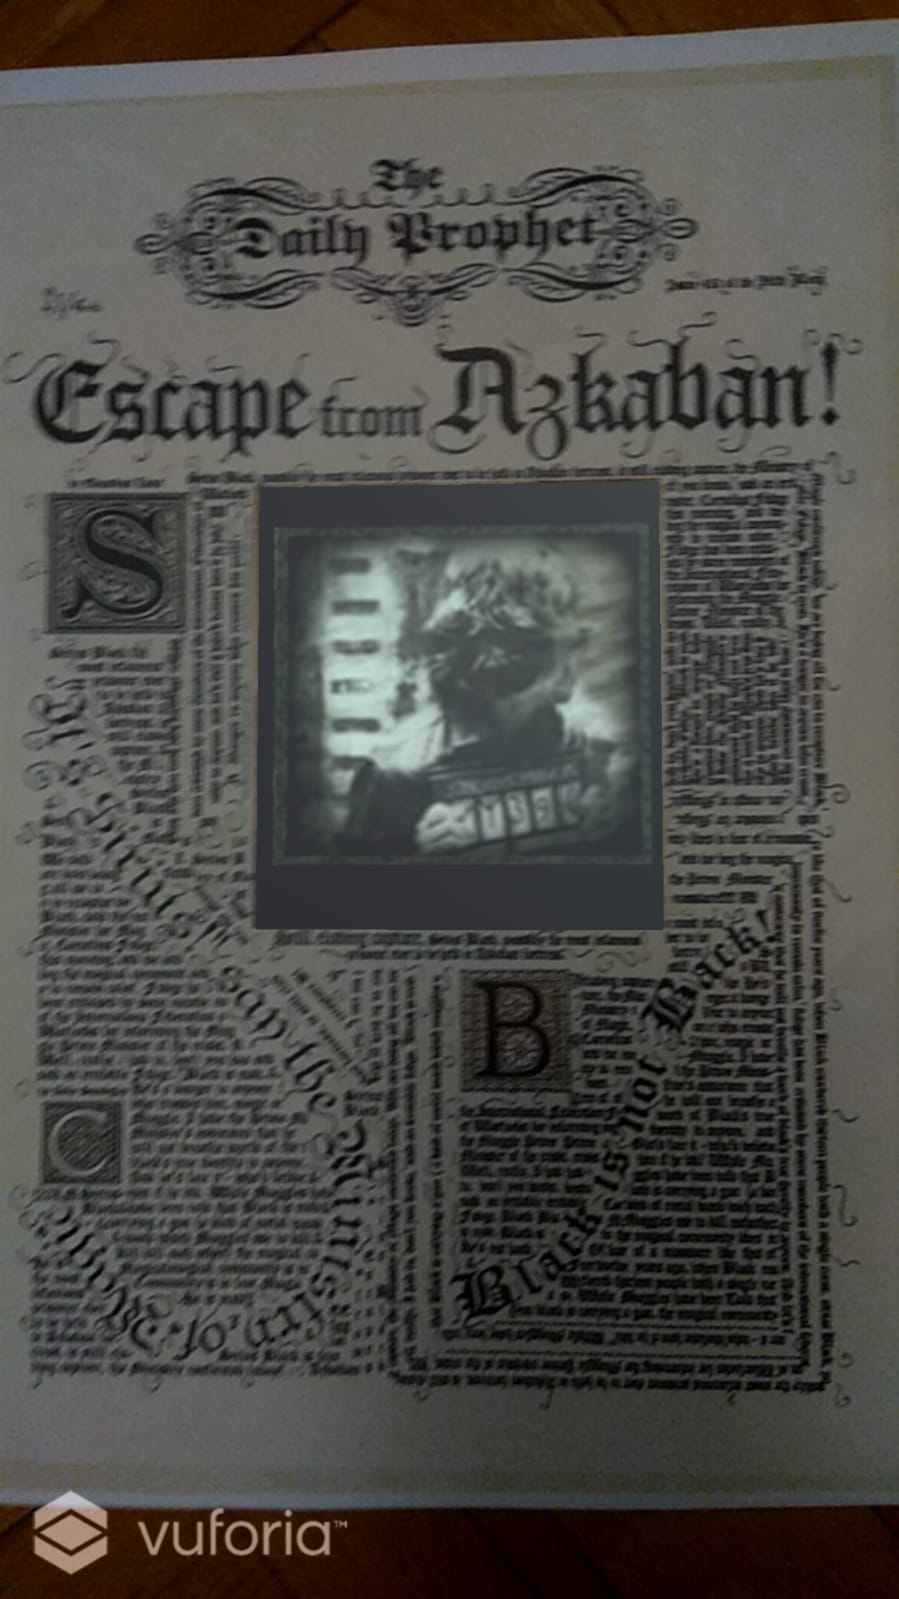
\includegraphics[width=0.4\linewidth]{Images/Azkaban.jpeg}
    \caption{Aplicación del periódico de Harry Potter}
    \label{Azkaban}
\end{figure}

Ahora viene el momento de utilizar Unity. Desde el editor, y con el paquete de Vuforia instalado procedimos a importar la base de datos que nos da Vuforia con la ilustración convertida en marcador. Realizar un uso básico y a modo de prueba de esta librería para el desarrollo de un ejemplo en realidad aumentada es bastante sencillo y animamos a cualquier persona que sienta curiosidad a seguir estos pasos, ya que solo requiere algunos conocimientos de cómo usar el editor de este motor de videojuegos.\\

Necesitamos en la escena un objeto que sea del tipo \textit{AR Camera}, que se encargará de renderizar la escena y detectar los marcadores. Usando este objeto podemos prescindir de la cámara tradicional. A continuación introdujimos el objeto \textit{Image Target}, también dentro del paquete de Vuforia y lo configuramos para que el componente \textit{Image Target Behaviour} utilice la base de datos que tenemos y la imagen que le corresponde. Como hijo del \textit{Image Target} incluimos el objeto virtual que queremos que aparezca al encontrar el marcador. En este caso, un objeto del tipo \textit{Quad} (es decir, un rectángulo vacío) nos servirá. Ajustamos el ancho y el alto al tamaño del padre y le añadimos el componente \textit{Video Player} para que reproduzca el gif animado. Con esto sólo necesitaríamos compilar la aplicación y pasar el archivo apk a un móvil que lo soporte para probar la aplicación.\\

\textbf{Se pueden ver los resultados en el video \url{https://vimeo.com/331236805}.}

\subsection{DragonBall}
La siguiente aplicación que desarrollamos está impulsada por la idea de leer un cómic en realidad aumentada. Utilizamos una página del manga de Dragon Ball para este ejemplo y le aplicamos básicamente el mismo procedimiento que al programa anterior, aunque con un par de excepciones.\\

En primer lugar, escogimos una página con unas viñetas lo suficientemente nítidas como para que los marcadores fueran de calidad. Una vez seleccionada (figura \ref{DBZ}) continuamos con el proceso de subida al servidor de Vuforia para obtener la base de datos. La parte difícil vino a continuación, pues tuvimos que encontrar el capítulo de la serie animada en el que sucedieran los hechos de esa página del cómic, para después recortar los fragmentos correspondientes a cada viñeta y ajustar el breve video de cada una al tamaño justo de la misma. Una vez teníamos todas las materias primas ya sólo había que introducirlas en el editor de Unity, creando esta vez cuatro \textit{Target Images} (uno para cada viñeta) y un \textit{Quad} con el video propio para cada uno.\\

Estamos especialmente contentos con esta demostración, ya que sin ser muy difícil de implementar, el resultado es muy vistoso y puede llegar a convertirse en una forma de ampliar la inmersión o mejorar la experiencia de los lectores habituales.
\begin{figure}[H]
    \centering
    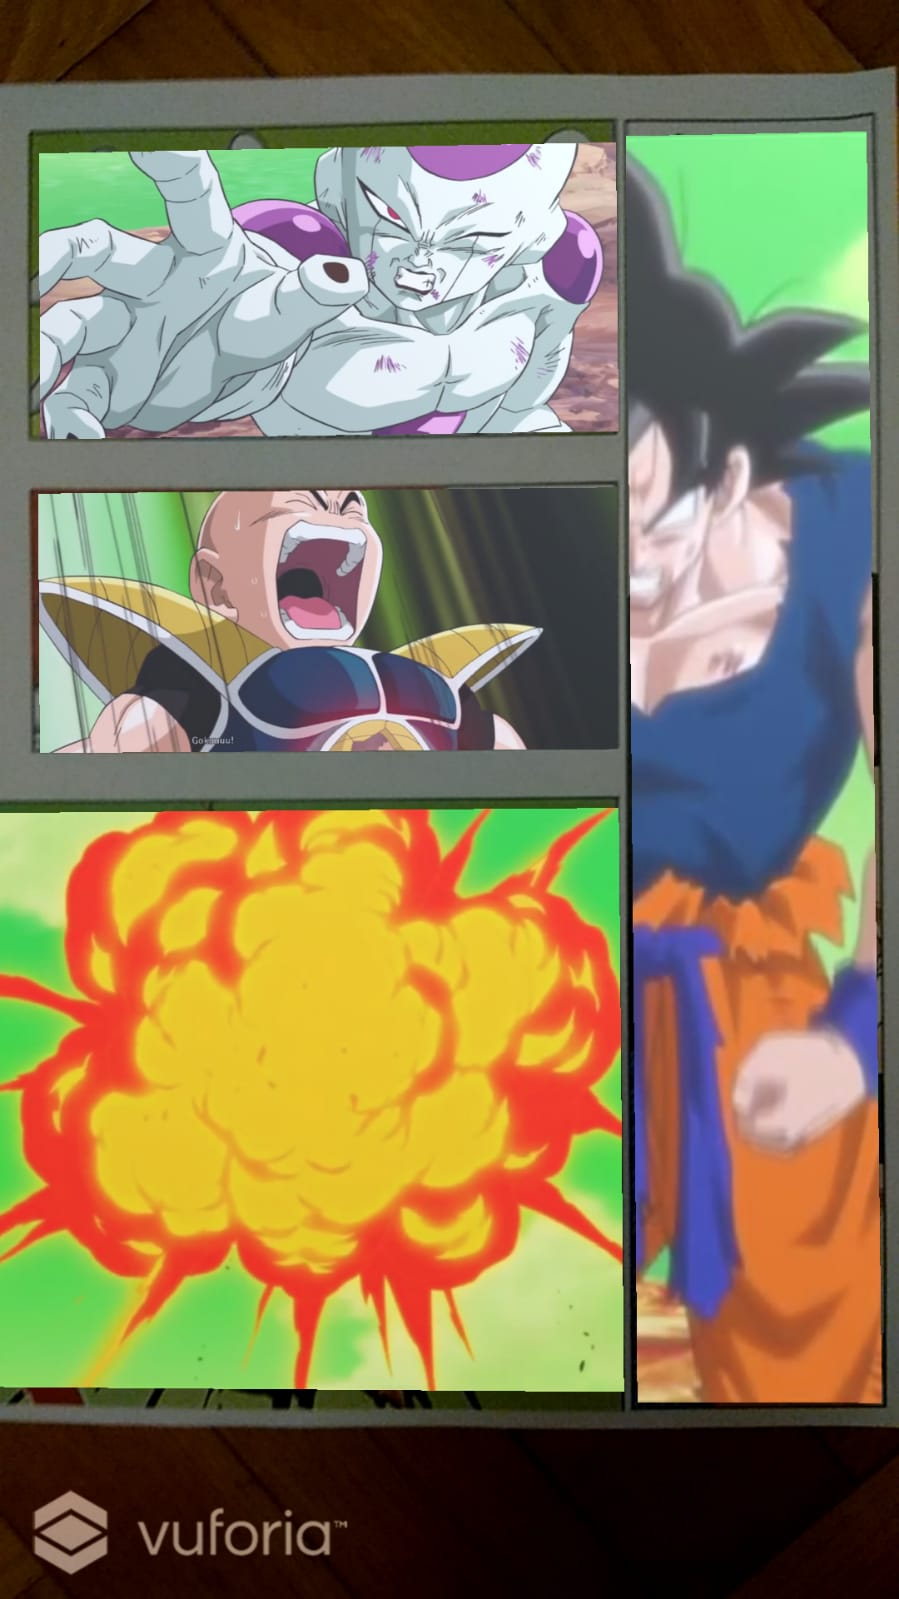
\includegraphics[width=0.3\linewidth]{Images/DragonBall.jpeg}
    \caption{Página del cómic con RA}
    \label{DBZ}
\end{figure}

Cabe destacar que actualmente la tecnología está limitada en este ámbito, ya que pese a que muchos dispositivos como tabletas o móviles soportan la realidad aumentada sin marcadores es de cierta manera incómodo tener que estar enfocando con la cámara al lugar en cuestión para obtener la información o la experiencia adicional y resulta cansado después de unos cuantos usos. Sin embargo, con dispositivos similares a las \textit{Google Glass}, que incorporen realidad aumentada y puedan llevarse siempre puestas, el mercado de este tipo de aplicaciones crecería radicalmente y se popularizaría enormemente su uso.

\textbf{Se pueden ver los resultados en el video \url{https://vimeo.com/331236593}.}

\subsection{Juego de cartas Yu-gi-oh}
Llegados a este punto, queríamos comprobar cómo sería el desarrollo de un juego que utiliza realidad aumentada con marcadores. Nos basamos para ello en el juego de cartas de Yu-Gi-Oh, que tiene su origen en un cómic japonés del mismo nombre y que alcanzó gran popularidad en la década de los 2000 en todo el mundo. El juego es de temática similar al de las cartas Magic, en el que cada carta representa un monstruo, cada uno con sus propios atributos, valores de ataque y defensa y otras características, que se enfrentan contra los monstruos del oponente siguiendo un sistema de reglas y turnos bastante complejo. Además de las cartas de monstruo existen otras que modifican los valores de las mismas o tienen otros efectos en la partida. Para facilitar el desarrollo, simplificamos todas estas condiciones y nos centramos en algunos aspectos esenciales: la partida se va sucediendo por turnos, las criaturas pertenecen a uno u otro jugador según su posición en la mesa y dentro de un turno el jugador puede decidir si el monstruo que está bajo su control ataca o defiende.\\

Lo verdaderamente interesante de este juego es que en la saga de cómic (y posterior serie animada de televisión) los jugadores juegan sobre un tablero electrónico sobre el que colocan las cartas y aparece una representación holográfica de las criaturas de las mismas. Esta tecnología de ciencia ficción se escapa un poco de nuestro alcance y presupuesto, pero sí que podemos intentar una recreación más simple con nuestros conocimientos de realidad aumentada y ver a los monstruos por medio de la pantalla de nuestros dispositivos móviles, como ya hicieron anteriormente juegos como Pokémon Go en 2016 o Invizimals en 2009.\\

Para desarrollar esta aplicación volvimos a utilizar el motor Unity con Vuforia. Utilizamos dos cartas del juego como marcadores para que durante el uso del programa proyectaran los modelos 3D de los monstruos correspondientes. Para los modelos buscamos algunas de las criaturas más conocidas de la franquicia y así evitamos tener que realizar nosotros a mano el proceso de modelado y generación de texturas. Encontramos en la página ``The model resource'' \footnote{ \url{https://www.models-resource.com}} los personajes que buscábamos (Kuriboh y Jinzo) y seleccionamos las cartas con sus imágenes para crear la base de datos que contendría los marcadores.\\

Encontramos un problema con los modelos,  carecían de animaciones; y es algo importante, ya que cada posible estado de las criaturas debía verse representado gráficamente por medio de una animación, además de que estas aportarían vitalidad y dinamismo al juego. Por todo esto, nos aventuramos a utilizar Blender, un programa de modelado, iluminación, renderizado y animación entre otras muchas características con el que estamos familiarizados por su uso en varios proyectos durante el grado y que además es software libre.\\

Por suerte los modelos llevaban en sí un \textit{rigging} básico (esqueleto animable), de manera que pudimos saltarnos la fase de creación del mismo. Realizamos animaciones de estado de reposo, ataque, defensa, movimiento y de recibir daño para ambas criaturas, además de las transiciones entre estos estados para evitar saltos poco realistas e incómodos en la simulación. Una vez guardadas todas las animaciones, el propio archivo de Blender puede ser directamente importado a Unity para utilizar todos los objetos y texturas que se encuentran en él. Esto nos facilitó mucho el trabajo al no tener que convertir los modelos a otro formato con la posible pérdida de información en los modelos o las animaciones. Una vez dentro del editor creamos los objetos que servirán como marcadores y les asignamos a cada uno su imagen correspondiente de la base de datos proporcionada por Vuforia. Como objeto hijo de cada marcador, le asignamos la figura correspondiente y creamos un \textit{prefab} con todo ello, ya que de querer ampliar el juego con más cartas cada una debería hacer referencia a un monstruo distinto.\\

Llegó la hora de ponernos a codificar. Establecimos un objeto vacío que sirviese de \textit{Game Manager} y llevase la lógica del juego, es decir, el transcurso de los turnos y las elecciones del jugador. Para empezar a jugar se sitúan las cartas sobre la mesa, una frente a la otra. Basándose en la orientación inicial de los marcadores cuando son detectados por la cámara, el juego asigna cada criatura al jugador al que le pertenece. Una vez pasada esta fase de reparto, le toca el turno al primer participante, que debe seleccionar uno de los monstruos en su control. Una vez hecho esto, aparecen tres botones en la pantalla: dos de ellos son para decidir si la criatura debe atacar o defender y el tercero cancela la selección y vuelve a la fase en la que se pide que escojas un monstruo. Si escoges atacar, el siguiente paso será buscar al objetivo del ataque, para lo que se pedirá seleccionar uno de los enemigos. Acto seguido, tu criatura se dirigirá a la del rival, la atacará haciéndole daño (que repercutirá en sus puntos de vida) y volverá a su carta de origen para pasar al turno del contrincante. Si por el contrario se elige la opción de defensa, el monstruo adoptará una postura defensiva que le permitirá cubrirse de los ataques enemigos y al acabar terminará el turno actual. A continuación será el turno del rival, que tendrá las mismas posibilidades, aunque en este caso jugaremos contra la máquina y sus acciones serán reducidas.\\

Para gestionar todo el grafo de animaciones necesitamos un objeto \textit{Animator Controller} que lleve las condiciones para pasar de un estado al siguiente y volver para cada uno de los modelos. Todos estos cambios se recogen a nivel de código una vez pulsamos los botones de selección de acción.\\

\begin{figure}[H]
    \centering
    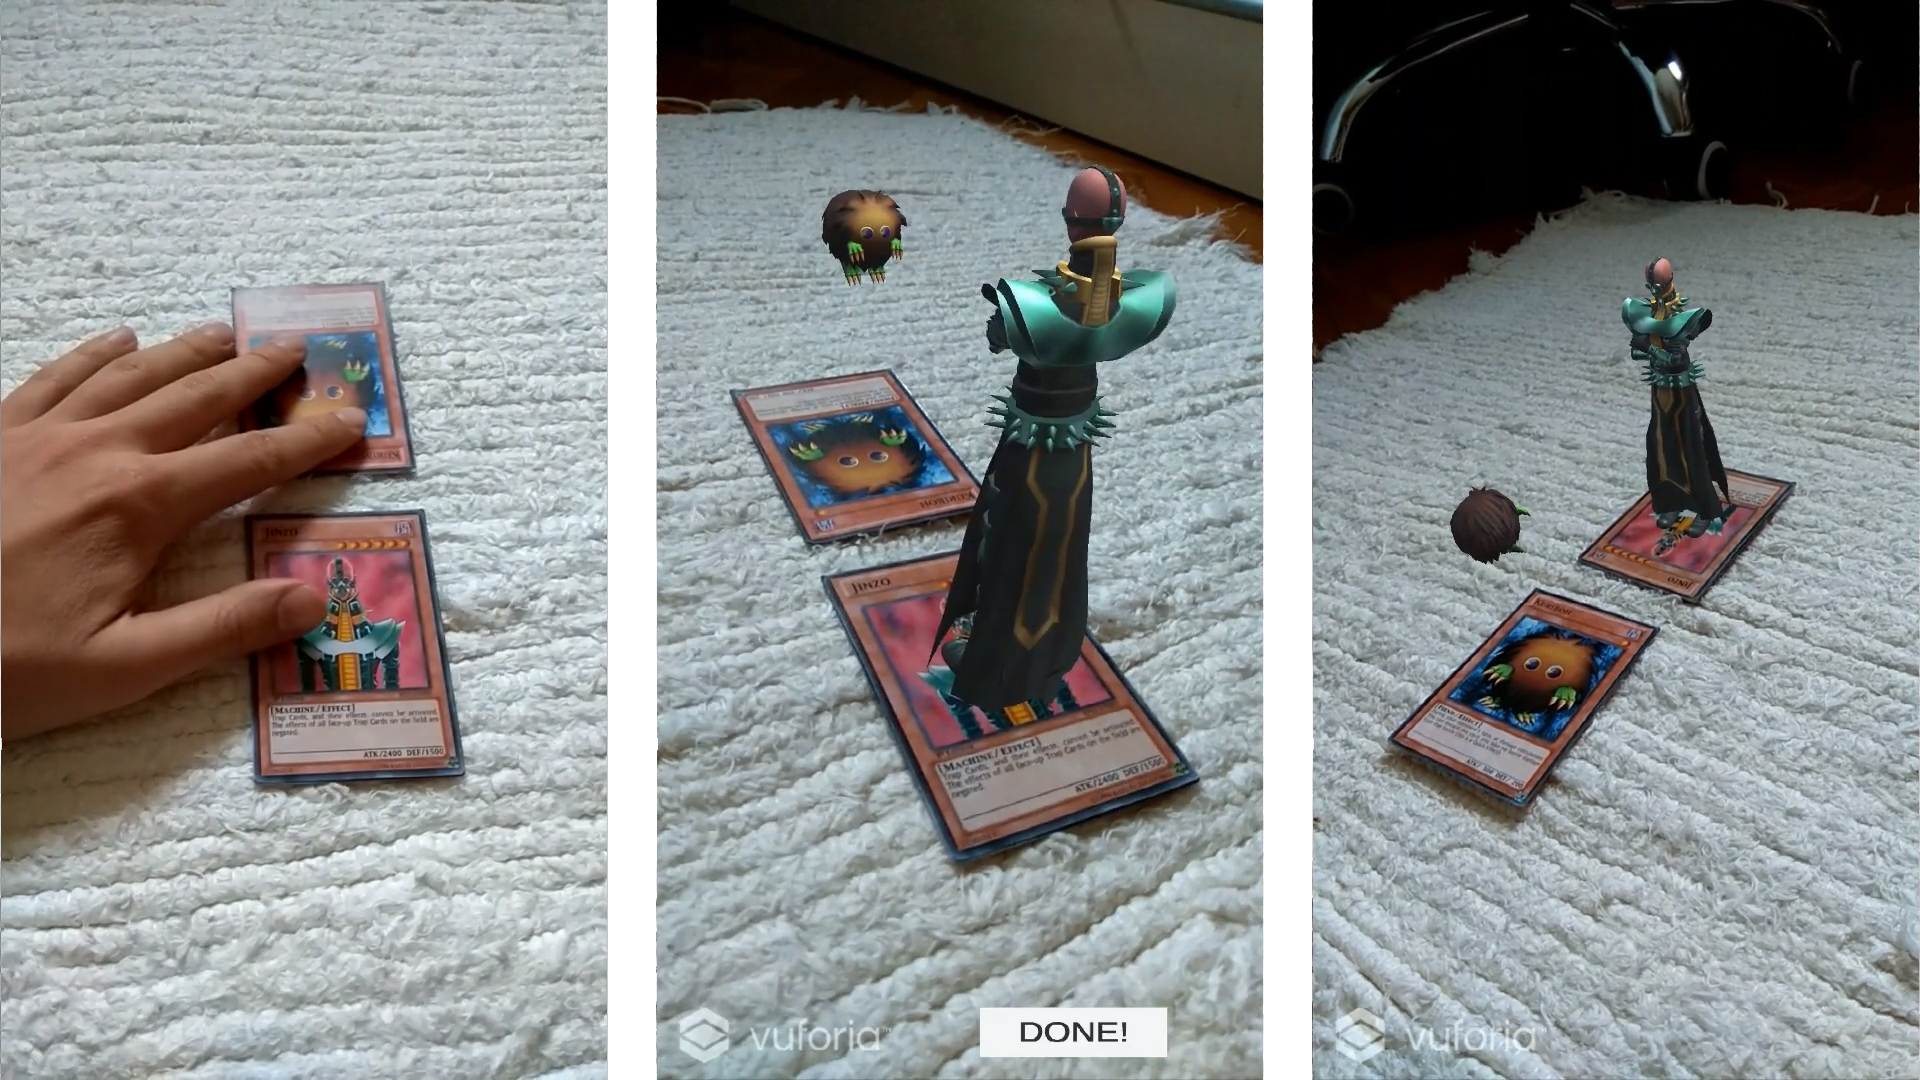
\includegraphics[width=\linewidth]{Images/YuGiOh.jpg}
    \caption{Visualización del juego de cartas}
    \label{YuGi}
\end{figure}

\textbf{Se pueden ver los resultados en el video \url{https://vimeo.com/331237916}.}\\

Con estas pequeñas muestras habríamos terminado nuestra incursión en la realidad aumentada con marcadores y estaríamos preparados para el siguiente paso, en el que prescindiríamos de ellos.

\newpage
\subsection{JengAR}
Una de las opciones para el juego multijugador online fue implementar el famoso juego de mesa Jenga\cite{jenga} en realidad aumentada con \textit{cloud anchors}. \\
Decidimos desarrollar un prototipo rápido donde se instancia una pila de bloques en un plano. Si nos acercamos un bloque y mantenemos pulsado la pantalla, el bloque se ancla a nuestro movimiento, por lo que hay que realizar movimientos suaves y cuidadosos, para no tirar la torre.\\
Cuando se pulsa la pantalla se calcula el punto que se encuentra en la mitad de la pantalla y se lanza un \textit{raycast} \footnote{Rayo que se lanza desde un punto origen hasta un punto final para comprobar si existe algún elemento en el camino}, si éste detecta un bloque, se marca como seleccionado, se fija la distancia entre su posición y la nuestra, y empieza a moverse junto a nosotros, manteniendo la distancia inicial.\\
En la figura \ref{JenAR} se pueden observar algunas capturas de la aplicación.
\begin{figure}[H]
    \centering
    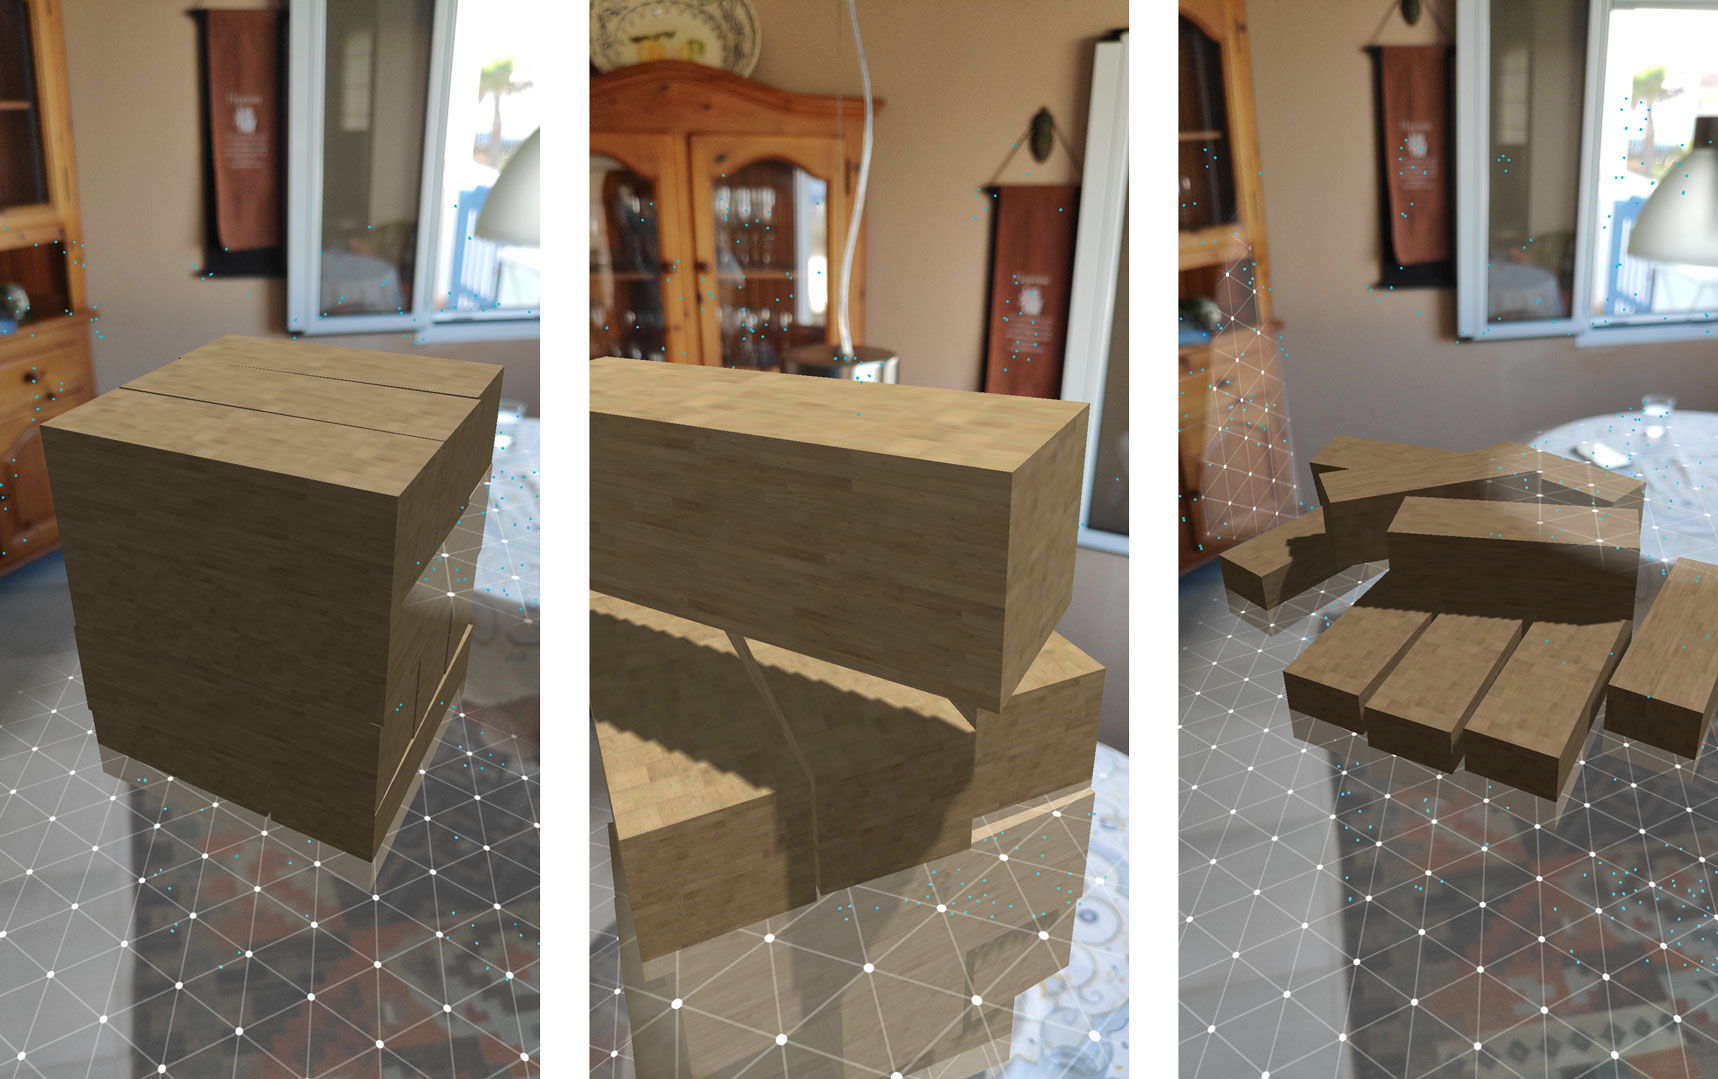
\includegraphics[width=\linewidth]{Images/Jenga.jpg}
    \caption{Visualización del JengAR}
    \label{JenAR}
\end{figure}
Optamos por abandonar el desarrollo debido a su poca complejidad, ya que la implementación era demasiado sencilla, por lo que no llegamos a implementar la mecánica de turnos ni la detección de victoria o derrota.\\

\newpage
\section{Juego multijugador con \textit{cloud anchor} - BombARdero+}
La tecnología que mas nos ha impresionado ha sido los \textit{Cloud Anchors}, nunca habíamos oído hablar de ella. Cuando nos enteramos de su existencia, estábamos todos de acuerdo en desarrollar un videojuego multijugador \textit{online}.\\

Los Cloud Anchors, como hemos explicado anteriormente, se almacenan en la nube de Google. Para usarlos, hace falta conseguir una clave de licencia de \textit{ARCore Cloud Anchor API} en Google Cloud Platform \cite{GCloud}. Una vez conseguida la credencial, hay que introducirla en Unity3D, ``Edit -> Project Settings -> Google ARCore -> Cloud Anchor API Keys''. En los ejemplos que ofrece Google, la implementación de los Cloud Anchor utiliza la \textit{Multiplayer High Level API(Multiplayer HLAPI)} de Unity, por lo que también hay que activar el servicio de multijugador en nuestro proyecto desde el \textit{dashboard} de Unity \cite{UnityDashboard}. Una vez realizado estos dos pasos, al compilar la escena de ejemplo, debería funcionar. En esa escena, un usuario tiene que crear una sala e instanciar un objeto, el punto de anclaje principal, que se convertirá en las coordenadas (0,0,0) del entorno.
Este punto de anclaje tarda unos diez segundos en subirse a la nube y estar disponible para más usuarios, que al entrar a la aplicación le aparece un listado con las salas disponibles. \\

Para desarrollar este juego, primero desarrollamos dos aplicaciones anteriormente.

Como al principio no teníamos dos móviles que soportasen ARCore, programamos el juego en monojugador, para acostumbrarnos al entorno y para ahorrarnos trabajo en un futuro.\\

En paralelo, como teníamos que implementar la parte de multijugador online y no teníamos ningún tipo de experiencia, realizamos unas pruebas para estudiar el funcionamiento de la Multiplayer HLAPI. Esas pruebas nos permitieron entender y aprender a desarrollar el multijugador de la prueba de concepto que nos hemos puesto como objetivo.\\

Una vez que conseguimos tener dos dispositivos que soportasen ARCore, empezamos a desarrollador la aplicación multijugador. Gracias a haber desarrollado el \textit{BombARdero}, nos permitió avanzar muy rápido ya que estaban los modelos, \textit{prefabs}\footnote{ Objetos prefabricados de Unity3D}, y scripts con las mecánicas básicas ya creadas. Primero tuvimos que mirar como estaba montada la implementación de Google, para entender el proceso de cómo se subía el marcador a la nube y la cantidad de información de control que teníamos. Este proceso fue bastante sencillo, ya que el código de ejemplo es muy entendible e intuitivo. Una vez conseguido implementar el BombARdero con los Cloud Anchors, hubo que hacer unos pequeños retoques a los scripts y añadir componentes de la multiplayer HLAPI a los objetos, para implementar la parte multijugador.\\

En el \textit{Cloud Anchor Network Manager} hay que registrar el objeto que se va a instanciar cada vez que entra un jugador a la partida, en nuestro caso será un avión. El avión en un principio está desactivado y se activa en el momento en el que se \textit{hostea} o resuelva el anchor principal. El avión consta de una velocidad constante hacia delante, y para controlar su trayectoria existe en la parte inferior izquierda de la pantalla un \textit{joystick} que te permite mover el avión hacia arriba, abajo, derecha e izquierda. En la esquina inferior derecha se encuentra un botón que al pulsarlo, se lanza una bomba en la posición del avión, dicha bomba sirve para destruir los edificios que se encuentran en la ciudad. El objetivo principal del juego es destruir el mayor número de edificios posible.

La principal complicación fue implementar la parte de multijugador, ya que no teníamos conocimiento previo sobre el tema.


\clearpage
\section{Instrucciones de montaje de muebles en AR - AmueblAR}

En nuestra investigación hemos visto que una de las utilidades más populares actualmente en el campo de la realidad aumentada son las aplicaciones de decoración de interiores. Ikea, por ejemplo, ha lanzado Ikea Place, una aplicación de realidad aumentada para dispositivos móviles que permite visualizar cualquier habitación de tu casa con muebles virtuales. De esta manera podemos decidir si encajan con nuestro salón y si las medidas son las adecuadas para después comprar el mueble en la tienda física.\\

Este programa despertó nuestra curiosidad y pensamos que podríamos desarrollar una aplicación con una utilidad parecida, pero en este caso aplicada al montaje de los muebles. Sabemos que comprar sofás o estanterías por piezas es en ocasiones más barato y facilita enormemente el transporte, sin embargo la parte en la que muchos compradores experimentan problemas es a la hora de montarlos. Muchos son incapaces de ver en el plano de las instrucciones en qué lugar va cada tornillo o de qué forma se unen las patas. Por eso, la aplicación que nosotros hemos propuesto consiste en un pequeño manual de instrucciones en realidad aumentada sin marcadores. De esta manera se puede ver en todo momento el modelo 3D del mueble, rotarlo y además desplazarte alrededor de él para apreciar en detalle cada uno de los pasos en el proceso de montaje.\\

El funcionamiento es muy sencillo: para empezar escaneamos el plano para que el programa cree una superficie donde colocar el mueble. A continuación tocamos la pantalla en el lugar en el que queremos colocarlo. Ahora podemos rotar el mueble hacia izquierda y derecha para dejarlo en una posición en la que nos resulte cómodo acercarnos y alejarnos mientras vemos los pasos de montaje. Finalmente, al pulsar el botón de aceptar entramos en la fase de construcción. En ella tenemos un botón a cada lado de la pantalla: el de la izquierda retrocede al paso anterior y el de la derecha avanza al paso siguiente. Mientras se suceden las animaciones que van explicando cómo armar progresivamente el mueble el usuario puede moverse libremente con su dispositivo para apreciar los detalles e incluso retroceder si no ha entendido bien el paso a seguir.\\

Para el desarrollo hemos utilizado la librería ARCore, que permite el despliegue de realidad aumentada sin marcadores. Utilizando la tecnología que nos vienen dada por la librería buscamos una serie de puntos en el suelo que nos permitirán crear un plano virtual. Una vez generada esta superficie el plano se representa gráficamente en pantalla con la unión de los puntos. A continuación dividimos la aplicación en tres estados: despliegue, rotación y montaje.\\ 

Empezamos en la fase de despliegue, en la que el programa está continuamente esperando la interacción del usuario. Cuando se toca la pantalla, se comprueba si ha habido colisión con el plano virtual, y de ser así se instancia el mueble en el lugar en el que hemos tocado. Si este proceso se ha llevado a cabo con éxito, pasamos a la fase de rotación. Aquí aparecen dos botones azules a los lados de la pantalla y uno verde en la parte inferior. Los botones laterales llevan una referencia al mueble para que al ser pulsados lo roten en una u otra dirección. El botón inferior por otra parte nos sirve para comunicarle a la aplicación que estamos conformes con la posición actual del objeto y que puede pasar a la siguiente fase.\\ 

Finalmente nos encontramos con dos nuevos botones a los laterales, que como hemos explicado anteriormente se encargan de adelantar y retroceder los pasos de montaje. El sofá tiene un componente \textit{Animator Controller} que lleva el árbol de estados. Este árbol consta de 10 estados fijos, en los que se queda el mueble una vez ha terminado su animación correspondiente y 18 estados móviles o animaciones, que se reproducen cuando pulsas el botón de avanzar o retroceder. Para ello, existe una variable que controla el avance y otra que hace lo propio con el retroceso, que se anulan una vez se entra en un estado estático y se activan al pulsar el botón que corresponde, pasando así a la animación del paso siguiente o anterior.\\

Cabe destacar el proceso de creación del mueble en sí mismo, que en el caso del ejemplo se trata del sofá \textit{Kivik}. Como no era posible encontrar un modelo dividido en piezas y fácilmente animable tuvimos que modelarlo desde cero con la ayuda de la documentación que encontramos en la web de Ikea. El mueble consta de las siguientes piezas: el asiento del sofá, el respaldo del sofá, el asiento de la \textit{cheslong} \footnote{ Tipo de sofá que posee una prolongación lo suficientemente larga en forma de L como para soportar las piernas humanas.} y su respaldo, los dos brazos, dos escuadras, una pletina, ocho patas, dieciocho tornillos con sus correspondientes tuercas y arandelas, cinco cojines cuadrados y un cojín alargado para la \textit{cheslong}. Excluyendo los tornillos, que los encontramos en una página de recursos gratuitos \cite{tornillos}, todos los demás fueron creados por nosotros en Blender, herramienta de la que ya hemos hablado anteriormente. Una vez terminadas las piezas del sofá, las texturizamos con colores azules y aspecto de sofá, y por otro lado las piezas como los tornillos o las escuadras una textura metálica.\\

Pensamos que podríamos empezar a animar cada parte por separado dentro de un objeto conjunto del que fueran hijas todas las piezas, pero para que Unity pueda interpretar cada acción como propia de un objeto mayor a las partes es necesario hacer un \textit{rigging}\footnote{ Proceso de crear un sistema de controles digitales y agregárselos a un modelo 3D para que así pueda ser animado fácilmente y eficientemente} que abarque todas piezas del sofá. Una vez construido el esqueleto hay que asignarle a cada hueso el objeto que se va a encargar de mover, lo cual dio también algunos problemas, ya que al tratarse de un objeto conjunto ciertos huesos acababan emparentándose automáticamente con partes del sofá que nos les correspondían, de modo que la única solución fue establecer manualmente los pesos (es decir, la influencia que tiene cada hueso sobre una parte concreta) sobre los diferentes conjuntos de vértices hasta que conseguimos el resultado que esperábamos.\\

En lo referente a las animaciones nos fue muy útil el vídeo que tiene publicado la cuenta de Ikea España en la plataforma Youtube \cite{IkeaYT} en el que se explica el procedimiento que se sigue para construir el sofá. Habiéndolo analizado dividimos el montaje en 9 pasos diferenciados y los animamos también en Blender, haciendo desaparecer las partes que no se están utilizando en ese momento para que sea más claro y fácil verlo.\\

Al contrario que en los ejemplos con marcadores en los que pudimos exportar directamente el archivo de Blender para su uso en Unity, aquí nos dio problemas ya que el editor dejó de reconocer los \textit{clips} de vídeo de algunas animaciones. Solventamos este problema exportando el objeto desde el programa de modelado en formato ``fbx'', pero nos surgió otro nuevo inconveniente, todas las partes del sofá habían perdido sus texturas. Ya desde Unity creamos los materiales por separado y se los asignamos a cada pieza.
Fue un proceso bastante agotador, sobre todo en la parte artística, pero consideramos que el resultado es satisfactorio y útil, además ofrece nuevas posibilidades en un campo que no deja de crecer.

\clearpage
\section{Visualizador de objetos en AR con gafas Aryzon}
En la fase de investigación, pensamos que una de las limitaciones de la realidad aumentada en dispositivos móviles es el hecho de tener que que estar sujetando el móvil con las manos, por lo que el control y la experiencia de usuario se ve condicionada negativamente. Decidimos buscar un headset de realidad aumentada encontramos las gafas de Aryzon \cite{Aryzon}, compramos un ejemplar y probamos qué tal funcionaban.\\

Descargamos las aplicaciones y juegos que promocionan para ver como era la experiencia usando las gafas. Nos resultó curioso y decidimos desarrollar una aplicación en la que se pudiera ver objetos y/o modelos 3D y poder caminar alrededor de ellas. Para añadirle más funcionalidad, usamos un mando de \textit{Xbox One} que nos permitirá mover, rotar y escalar el modelo a nuestro gusto, con el objetivo de poder manipular la aplicación sin necesidad de tocar el móvil, ya que éste estará colocado en las gafas.\\

Para el desarrollo de la aplicación usamos el SDK de Aryzon, que nos facilita la vista estereoscópica\footnote{ Dos puntos de vista poco separados entre sí} para simular nuestros ojos, ya que las gafas están compuestas por dos espejos que reflejan la imagen al cristal por donde nosotros vemos el mundo real, permitiendo tener esa visión de realidad aumentada como se puede observar en la figura \ref{GafasAryzon}.

\begin{figure}[H]
    \centering
    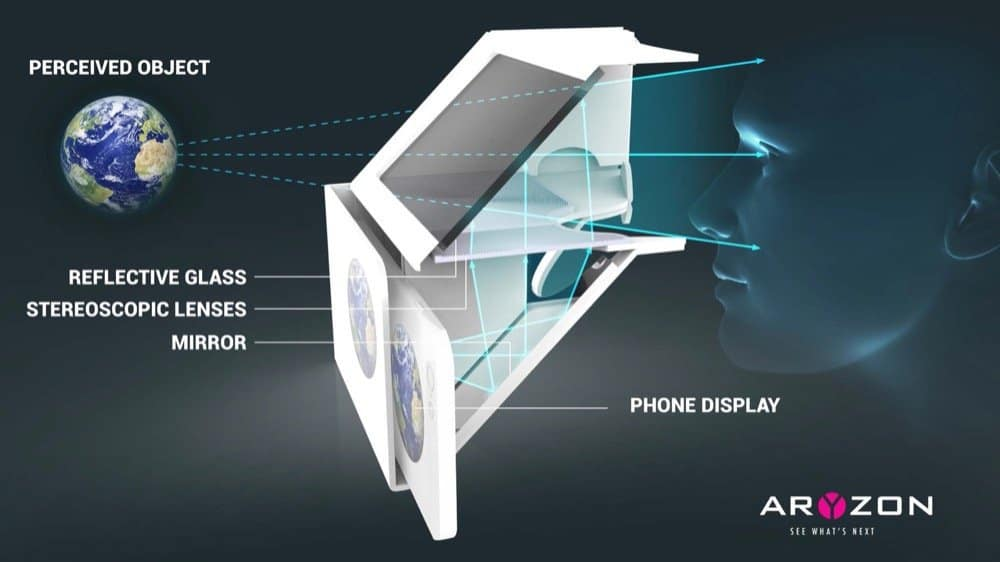
\includegraphics[width=0.75\linewidth]{Images/How-it-works.jpg}
    \caption{Como funciona las gafas de Aryzon}
    \label{GafasAryzon}
\end{figure}
 {\let\thefootnote\relax\footnote{{Imagen de la figura \ref{GafasAryzon} sacada de https://www.igadgetsworld.com/aryzon-diy-augmented-reality-headset/}}}

Todos los ejemplos que proporciona Aryzon son con marcadores o no usan de verdad realidad aumentada, si no que que es una escena de realidad virtual con fondo negro y vista esteoroscópica, entonces da el efecto de ser realidad aumentada, pero la aplicación en sí es realidad virtual. Nosotros hemos decidido usar ARCore, ya que queremos usar la realidad aumentada sin marcadores y movernos alrededor del modelo, y como hemos visto en las pruebas, la estabilidad de los puntos de anclaje de ARCore es muy buena.\\
Para el desarrollo de esta prueba de concepto, necesitamos el SDK de Aryzon y el SDK de ARCore, y los modelos sacados del \textit{Asset Store} de Unity \cite{AssetStore}. Desarrollamos un \textit{script} para manipular con el mando de Xbox One los objetos que instanciamos. El joystick izquierdo sirve para mover el objeto en los ejes X y Z, para moverlo verticalmente, se usa la cruceta (D-PAD) vertical. Para rotar el objeto en cuestión hemos configurado el script para que se realice con el joystick derecho, y para finalizar, con la cruceta horizontal podemos escalar el objeto. Por otro lado, los botones con los que controlamos la creación de objetos son, la A que permite instanciar el objeto en el lugar en el que estemos mirando, la X que cambia el modelo que se va a instanciar, ya que hemos puesto seis modelos en esta prueba de concepto y la B, nos permite activar y desactivar el \textit{render} de los planos que ha encontrado la aplicación, para tener una visión más limpia.\\
El mayor problema que nos encontramos al desarrollar la aplicación fue la documentación respecto al \textit{mapeo} del mando, ya que cambia según la plataforma en la que se utiliza. La de Android no estaba actualizada y no coincidían los botones y los ejes que nos proporcionaba la documentación.\\
El resultado final nos parece muy interesante, ya que tener el teléfono fijo en nuestros ojos gracias a las gafas, hace que podamos tener las manos libres para poder controlar y manipular lo que queramos ver. El precio de las gafas es un precio asequible para el público, y en nuestro caso hemos utilizado un mando de \textit{Xbox One} oficial, pero existen mandos Bluetooth para los \textit{smartphones} que también se pueden conseguir muy baratos. Usando la realidad aumentada de esta manera abre las posibilidades a nuevas mecánicas de juego y seguramente suponga una revolución en la realidad aumentada de "bolsillo".\\
Lo que se ve en la figura \ref{appAryzon} es la aplicación usando ARCore y el SDK de Aryzon, el modelo que vemos en la imagen, se proyecta a traves del sistema de cristales explicado anteriormente, permitiendo una visión del mundo real y el modelo 3D superpuesto en el plano encontrado.

\begin{figure}[H]
    \centering
    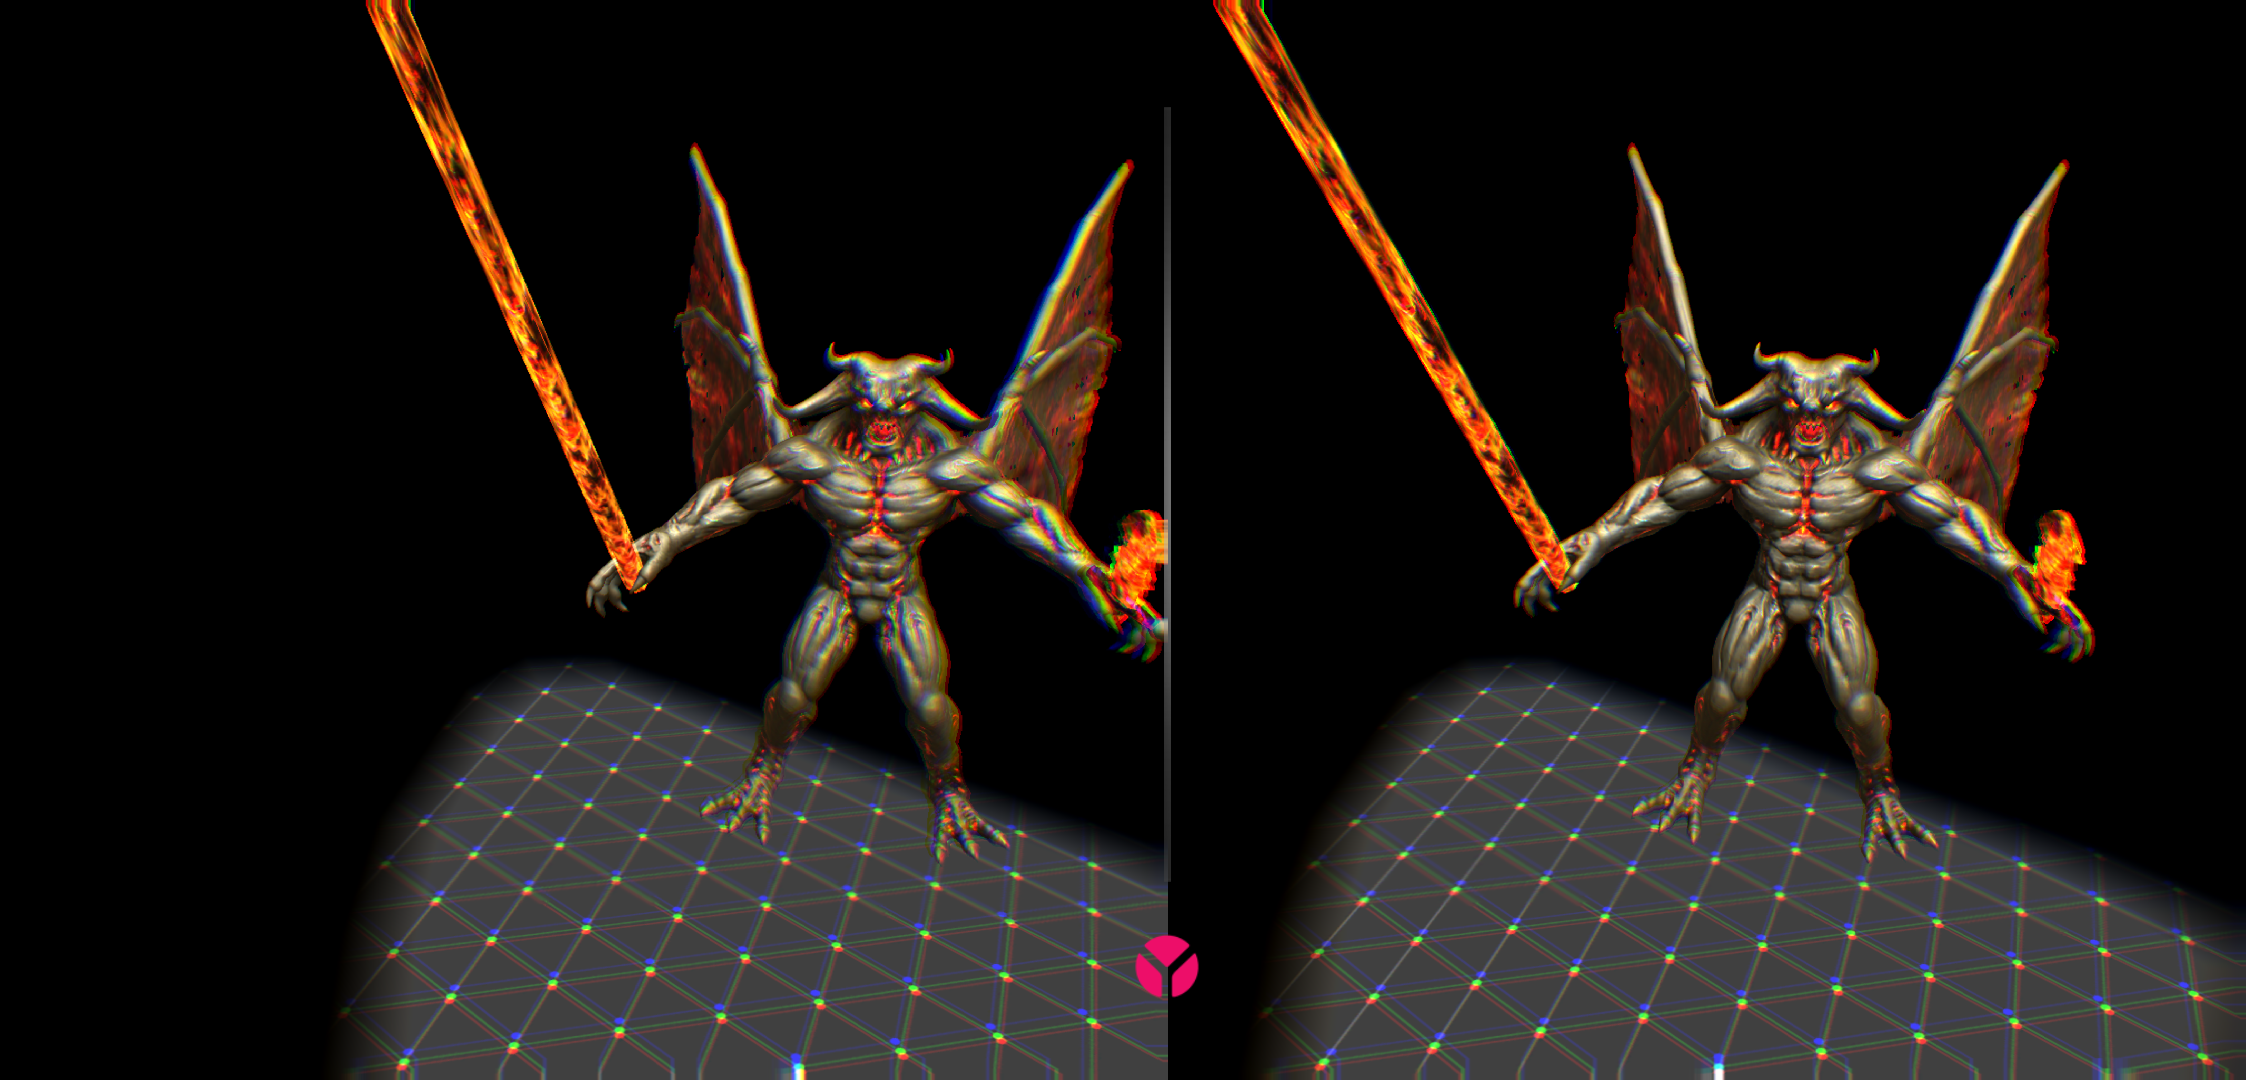
\includegraphics[width=0.75\linewidth]{Images/aryzonVisualizer.png}
    \caption{Proyección estereoscópica del móvil}
    \label{appAryzon}
\end{figure}
\noindent
\chapter*{Conclusiones}
\addcontentsline{toc}{chapter}{Conclusiones}

Tras la finalización del proyecto, podemos extraer varias conclusiones sobre las diferentes librerías expuestas en este trabajo, proporcionados tanto por los resultados obtenidos como por la investigación llevada a cabo durante estos meses.\\

Gracias a este estudio podemos hacer una estimación bastante certera de cuál es el estado, las capacidades y las limitaciones de las librerías y la tecnología de realidad aumentada actualmente cumpliendo de esta manera nuestro objetivo principal con creces.\\

El proyecto ha aportado nuevas conclusiones respecto al estado de la cuestión y los antecedentes de los que se parte.\\

Gracias a las pruebas desarrolladas con las principales librerías del mercado podemos establecer que Google y Apple lideran en calidad, por lo que ARCore y ARKit, son una de las opciones más viables para una aplicación que exige estabilidad y precisión. También cabe destacar el esfuerzo por parte del equipo de desarrollo de Unity3D para implementar la API de ARFoundation, que nos permite desarrollar aplicaciones de realidad aumentada para Android e iOS con el mismo código. 
Por otra parte, tenemos librerías ``low cost'' que son más inestables, pero son capaces de funcionar en casi todos los dispositivos \cite{wikitudeInstant} y en un gran porcentaje de entornos y condiciones. Esto hace que el uso de estas librerías, como puede ser Vuforia, EasyAR, o Maxst, sea una opción a elegir para aplicaciones que no requieran una estabilidad tan minuciosa.\\

Después de haber probado todas las librerías vistas anteriormente, queda de manifiesto que se ha conseguido que la estabilidad sea prácticamente perfecta en la mayoría de los casos. También observamos un gran avance en la estimación de luces, muy lograda en casos como ARCore y ARkit, aportando mayor realismo a la experiencia inmersiva. Concluimos que los desarrolladores de ambas empresas líderes (Apple y Google) están optando por revolucionar el mercado con tecnologías como la oclusión y los \textit{Cloud Anchors}. La realidad aumentada es una tecnología muy novedosa, por lo que avanza muy rápidamente, aproximadamente cada mes y medio ARCore recibe una nueva actualización, sin ir más lejos al realizar este trabajo hemos podido observar muchos cambios importantes en el funcionamiento de la librería.\\

Gracias a la extensa documentación existente y a los tutoriales creados por la comunidad, el aprendizaje del desarrollo de aplicaciones con realidad aumentada sin marcadores resulta cómodo y accesible para el desarrollador. Esta accesibilidad nos ha permitido el desarrollo de tres aplicaciones destinadas a tres sectores diferentes.


\section*{Futuros pasos}
\addcontentsline{toc}{section}{Futuros pasos}

Como futuros pasos podemos establecer seguir pendientes de la evolución de las librerías de cara a poder generar aplicaciones de mayor calidad. Por otro lado nos gustaría retomar algunas ideas que descartamos y seguir con el desarrollo de las pruebas de concepto, ya que nos parecen de gran utilidad y el videojuego creado utiliza mecánicas nuevas nunca vistas. Las pruebas que hemos realizado siempre han sido en interior, nos gustaría probar el funcionamiento de las librerías en exterior y ver cómo se comportan.

\noindent 

\chapter{Capítulo 6}
\noindent

\chapter{Contribuciones}
\section{Colin Ulrich Cop}
Antes de empezar el proyecto, tuve mis primeros pasos desarrollando aplicaciones de realidad aumentada con marcadores usando la librería Vuforia. Más tarde, adquirí un teléfono que soportaba ARCore por lo que empecé a probar la realidad aumentada sin marcadores.\\

Las primeras aplicaciones desarrolladas consistían en instanciar diferentes objetos y hacer que interactuasen entre ellos. Empecé a investigar sobre las librerías disponibles y las iba probando, sobretodo 8thWall,que aún no tenía el SDK abierto y tuve que enviar una solicitud personal, con esta librería, también pude probar la realidad aumentada en la web. Durante el curso, en la asignatura \textit{Videojuegos en dispositivos Móviles}, impartida por Pedro Pablo Gómez Martin, tuvimos que programar el juego Bombardero Amstrad-CPC, una vez terminada la práctica, me pareció buena idea desarrollar dicho juego en realidad aumentada. Una vez implementadas las mecánicas básicas, el desarrollo se quedó pausado. También hice el prototipo de JengAR visto anteriormente, que no lo terminé ya que debido a su baja complejidad, no íbamos a implementar la versión multijugador. Otro de los prototipos que realicé fue un juego plataformas en el que se controlaba con el mando y se apuntaba con la cámara, estaba pensado para ser jugado con un mando bluetooth y un soporte del móvil para dicho mando. \\

Cuando descubrimos la existencia de los \textit{cloud anchors}, aún no disponíamos de dos dispositivos en los que poder probar esa tecnología, pero decidimos que una de las pruebas de concepto iba a ser un juego multijugador \textit{online} usando los \textit{cloud anchors}. Me empecé a informar respecto a cómo hacer un juego multijugador en Unity, por lo que estuve aprendiendo la \textit{Multiplayer High Level API}, y por otro lado también usé el plugin Photon\cite{pun}, porque vi que se usa mucho y es más completo que la API de Unity3D. Me encargué de crear las aplicaciones usando todas las librerías, exceptuando ARKit y Vuforia, para el posterior análisis de cada una. Dicho análisis fue realizado junto a Patricia, los dos nos reunimos para probar todas las aplicaciones en el mismo entorno y mismas condiciones. Junto a Patricia encontré las gafas Aryzon\cite{Aryzon}, y se nos ocurrió crear una aplicación en la que pudieras observar y manipular objetos 3D.\\

Cuando la facultad nos proporcionó un teléfono que soportase ARCore, pude empezar la prueba de concepto BombARdero+, que se pudo adaptar bien a los cloud anchors gracias a que ya tenía un proyecto con los prefabs y scripts hechos anteriormente. Patricia me ayudó a adaptar dicho proyecto al multijugador y a implementar las funcionalidades requeridas para que funcionase correctamente \textit{online}.\\

Con respecto a la memoria, antes de empezar a escribir, me informé en varios libros y webs sobre la historia de la RA, ya que me encargué de escribir la definición e historia. Por otro lado, tuve que estudiar varias tecnologías implicadas en la RA sin marcadores,como el SLAM, detección de planos, reconocimiento del ambiente, oclusión, estimación de luces, e hice un estudio completo sobre las funcionalidades y licencias de cada librería que hemos visto . Patricia y yo hemos realizado el capítulo 3 entero, donde tuvimos que someter cada una de las aplicaciones a un test y evaluar su rendimiento en diferentes condiciones de luz. Finalmente, junto a Patricia, traduje la introducción y las conclusiones al inglés.
\newpage
\section{Patricia Cabrero Villar}
Mi primer contacto con la realidad aumentada fue cuando realicé mi trabajo fin de grado cuando cursé el Grado de Diseño Gráfico y Multimedia, donde desarrollé una aplicación de realidad aumentada con marcadores específica para niños con trastorno del espectro autista.
Después de esta primera aproximación al mundo de la realidad aumentada me pareció interesante continuar formándome y aprendiendo en lo que refiere a este campo, con lo que decidí proponer como tema la realidad aumentada sin marcadores.\\

Una vez establecido el tema investigué en busca de tecnologías disponibles y bibliografía actualizada para poder tener una base sólida sobre la que apoyarme para el desarrollo del proyecto. De esta manera surgieron títulos como \textit{Handbook of Augmented Reality} de Carmigniani y Furth que me ayudó a comprender con mayor profundidad la tecnología a tratar y como punto de  referencia del paradigma actual establecí el libro \textit{Augmented reality games II, The gamification of education,medicine and art} de Geroimenko.\\

Realizada la investigación fui la encargada de establecer la estructura y plan de trabajo que seguiríamos a lo largo del proyecto para poder llevar a cabo los objetivos propuestos conjuntamente. En un primer paso plasmamos entre los tres los conocimientos adquiridos en la fase de investigación mostrando los antecedentes, historia y librerías de realidad aumentada en el primer y segundo capítulo.\\

Más tarde definí las pruebas y características que observaríamos en los \textit{test} de las diferentes librerías junto con mi compañero Colin. El desarrollo de las aplicaciones se dividió de manera que yo realicé las apps de Vuforia y ARKit ya que era necesario un dispositivo iOS para su correcto funcionamiento. Una vez tuvimos desarrolladas todas las pruebas de las librerías se probaron todas bajo las mismas condiciones de luz y tecnología, esta evaluación fue llevada a cabo por Colin y por mí. Estableciendo conjuntamente las puntuaciones y conclusiones de cada librería. Gracias a estas pruebas Colin y yo pudimos establecer una evaluación global de las librerías actuales y con estas conclusiones decidir las pruebas de concepto que desarrollaríamos en una segunda fase.\\

Por último, en esta segunda fase se decidió desarrollar una aplicación multijugador(BombARdero+), una inmersiva(Aryzon) y una descriptiva(AmueblAR). El desarrollo de estas aplicaciones se decidió dividir entre los integrantes ya que permitía un desarrollo más ágil y debido a la necesidad de dos teléfonos en el caso del multijugador. Debido a esto realicé junto con mi compañero Colin la aplicación multijugador BombARdero+ y el visualizador de objetos en 3D para las gafas Aryzon. En el caso de la aplicación multijugador focalicé mis esfuerzos en comprender el funcionamiento de la API de multijugador de Unity para poder utilizarla en consonancia con los \textit{cloud anchors}. Mi papel en el desarrollo de la visualización de objetos con las gafas Aryzon fue el de investigar acerca de la posibilidad de implementar la visión estereoscópica junto con ARCore.


\newpage
\section{David González Jiménez}
Dado que al inicio del trabajo la tecnología de mi móvil era la más anticuada y la única que no soportaba el uso de librerías que permitiesen trabajar con realidad aumentada sin marcadores, mis primeros pasos consistieron en documentarme y utilizar librerías preparadas para funcionar con marcadores, como Vuforia y ARToolKit.\\

En una primera incursión con ARToolkit pude encontrar un paquete que lo integraba en Unity y una documentación bastante precaria sobre cómo utilizar este \textit{plugin}. Tras unas cuantas búsquedas conseguí hacer una aplicación muy básica que funcionase en mi dispositivo a modo de aproximación, que está explicada en la sección correspondiente a las pruebas con ARToolKit.\\

Ahora que ya había tocado los orígenes de la realidad aumentada podía ponerme manos a la obra con la librería
Vuforia, también integrada en Unity. Por este entonces seguía sin tener acceso a tecnología que permitiese ejecutar aplicaciones de realidad aumentada sin marcadores, de manera que los prototipos que realicé en con esta librería también utilizaban marcadores. Sin embargo, los resultados fueron mucho más satisfactorios y vistosos porque Vuforia pone a la disposición del desarrollador gran cantidad de herramientas que hacen el trabajo más sencillo y dan mejores resultados. Los prototipos que realicé en este caso fueron dos aplicaciones para el visionado de vídeos virtuales sobre imágenes reales que se exponen en detalle en los apartados correspondientes a las pruebas con Vuforia con marcadores. Pude hacer con éxito un cartel animado basado en la saga de Harry Potter y una página de cómic de DragonBall en la que se reproduce un pequeño vídeo en cada viñeta.\\

En última instancia, y con el fin de hacer una aplicación algo más compleja con marcadores hice la implementación de un juego de cartas por turnos en la que las criaturas que están dibujadas en los naipes aparecen como modelos 3D al verlas a través de un móvil. El juego consta de turnos y sería multijugador de haber insistido en dejarlo completamente cerrado, sin embargo, al ser un prototipo de aproximación el rival es controlado por una inteligencia artificial. Todo este desarrollo puede leerse en la sección correspondiente en el capítulo del juego implementado en realidad aumentada con marcadores.\\

Finalmente, la facultad me proporcionó un móvil que permitía por fin el despliegue de aplicaciones que usan realidad aumentada sin marcadores, así que mis compañeros y yo nos repartimos diferentes aplicaciones para realizar en ellos. Yo escogí basándome en el concepto de Ikea Place una aplicación que sirviese como manual de instrucciones para cualquier usuario que quisiera montar un mueble en su casa. La aplicación de momento consta de un sofá cuyo montaje se divide en 9 pasos diferenciados que el usuario puede pasar hacia delante y detrás, así como rotarlo o moverse alrededor de él a voluntad para facilitar la comprensión del ensamblaje. El proceso de desarrollo y la idea desarrollada se pueden consultar en la sección que habla sobre la aplicación AmueblAR.\\

Por último añadir que además del desarrollo de las aplicaciones anteriores, me he documentado sobre diferentes aspectos del funcionamiento de la realidad aumentada, como son los \textit{cloud anchors} o la detección de caras para escribir dichas secciones en la memoria, así como las diferentes aplicaciones y avances que se han producido recientemente en campos como la educación, el arte, la medicina, la publicidad o el turismo en relación a las tecnologías de la realidad aumentada, además de los diferentes métodos de \textit{tracking} existentes hasta el momento.\\

\noindent
%\input{Chapters/Chapter07en.tex}
%%%%%%%%%%%%%%%%%%%%%%%%%%%%%%%%%%%%%%%%%%%
%%%%%%%%%%%%%%%%%%%%%%%%%%%%%%%%%%%%%%%%%%% Parte 3 - Index y bibliografía
\chapter*{Repositorios}
\addcontentsline{toc}{chapter}{Repositorios}
\textbf{Repositorio principal: \url{https://github.com/ar-tfg/}}\\

Repositorio de la memoria: \url{https://github.com/ar-tfg/Memoria}\\

Repositorio pruebas de concepto: \url{https://github.com/ar-tfg/DemosLibrerias}\\

Vídeos de las pruebas de concepto: \url{https://www.youtube.com/playlist?list=PLqQgTAUiabc8AQrcc48Jdglnytus9IoXe43}\\

Repositorio de la aplicación Yu-gi-oh: \url{https://github.com/ar-tfg/Yu-gi-oh}\\

Repositorio de la aplicación de Harry Potter: \url{https://github.com/ar-tfg/HarryPotter}\\

Repositorio de la aplicación de Harry Potter: \url{https://github.com/ar-tfg/DragonBall}\\

Repositorio del juego JengAR: \url{https://github.com/ar-tfg/JengAR}\\

Repositorio del juego BombARdero+: \url{https://github.com/ar-tfg/BombarderoOnline}\\

Repositorio de la aplicación Visualizer3D: \url{https://github.com/ar-tfg/Visualizer3D}\\

Repositorio de la aplicación AmueblAR: \url{https://github.com/ar-tfg/AmueblAR}\\

\indiceFiguras
\indiceTablas
%%%%%%%%%%%%%%%%%%%%%%%%%%%%%%%%%%%%%%%%%%%
%%%%%%%%%%%%%%%%%%%%%%%%%%%%%%%%%%%%%%%%%%% Parte 4 - BIB y licencia
\biblioTFG{}

%\licenciaTFG{PASCAL}{ENERO 2018}{CC-ZERO}
%%%%%%%%%%%%%%%%%%%%%%%%%%%%%%%%%%%%%%%%%%%
\end{document}